\documentclass[runningheads]{llncs}
%
\usepackage{amsmath}
\usepackage{amssymb}
% \usepackage{booktabs} % For pretty tables
% \usepackage{caption} % For caption spacing
% \usepackage{subcaption} % For sub-figures
\usepackage[dvipsnames]{xcolor}
\usepackage{graphicx}
\usepackage{makecell}
\usepackage{array} % For centering text in tables with fixed width
\newcolumntype{x}[1]{>{\centering\arraybackslash\hspace{0pt}}p{#1}}
\usepackage{pgfplots}
\usepackage[all]{nowidow}
\usepackage[utf8]{inputenc}
\usepackage{tikz}
\usetikzlibrary{er,positioning,bayesnet}
\usetikzlibrary{automata, arrows.meta, positioning}
\usepackage{multicol}
\usepackage{algpseudocode,algorithm,algorithmicx}
\usepackage{minted}
\usepackage{hyperref}
\hypersetup{
    colorlinks=true,
    citecolor=red,
    linkcolor=blue,
    filecolor=magenta,      
    urlcolor=blue
}
\usepackage[inline]{enumitem} % Horizontal lists
% Used for displaying a sample figure. If possible, figure files should
% be included in EPS format.
%
% If you use the hyperref package, please uncomment the following line
% to display URLs in blue roman font according to Springer's eBook style:
% \renewcommand\UrlFont{\color{blue}\rmfamily}

\definecolor{col1}{rgb}{0.5529411764705883, 0.8274509803921568, 0.7803921568627451}
\definecolor{col2}{rgb}{1.0, 1.0, 0.7019607843137254}
\definecolor{col3}{rgb}{0.7450980392156863, 0.7294117647058823, 0.8549019607843137}
\definecolor{col4}{rgb}{0.984313725490196, 0.5019607843137255, 0.4470588235294118}
\definecolor{col5}{rgb}{0.5019607843137255, 0.6941176470588235, 0.8274509803921568}
\definecolor{col6}{rgb}{0.9921568627450981, 0.7058823529411765, 0.3843137254901961}
\definecolor{col7}{rgb}{0.7019607843137254, 0.8705882352941177, 0.4117647058823529}
\definecolor{col8}{rgb}{0.9882352941176471, 0.803921568627451, 0.8980392156862745}
\definecolor{col9}{rgb}{0.8509803921568627, 0.8509803921568627, 0.8509803921568627}
\definecolor{col10}{rgb}{0.7372549019607844, 0.5019607843137255, 0.7411764705882353}
\definecolor{col11}{rgb}{0.8, 0.9215686274509803, 0.7725490196078432}
\definecolor{col12}{rgb}{1.0, 0.9294117647058824, 0.43529411764705883}
\definecolor{lightgrey}{rgb}{0.83, 0.83, 0.83}
\pgfplotsset{compat=1.14}

\newcommand{\ind}{\perp\!\!\!\!\perp}
\newcommand{\notind}{\not\!\perp\!\!\!\perp}

\newcommand{\card}[1]{\left\vert{#1}\right\vert}
\newcommand*\Let[2]{\State #1 $\gets$ #2}
\renewcommand{\topfraction}{0.85}
\renewcommand{\bottomfraction}{0.85}
\renewcommand{\textfraction}{0.15}
\renewcommand{\floatpagefraction}{0.8}
\renewcommand{\textfraction}{0.1}
\setlength{\floatsep}{3pt plus 1pt minus 1pt}
\setlength{\textfloatsep}{3pt plus 1pt minus 1pt}
\setlength{\intextsep}{3pt plus 1pt minus 1pt}
\setlength{\abovecaptionskip}{2pt plus 1pt minus 1pt}

\begin{document}
%
\title{Chain Event Graphs - subtitle}
%
%\titlerunning{Abbreviated paper title}
% If the paper title is too long for the running head, you can set
% an abbreviated paper title here
%
\author{Katarzyna Kobalczyk\inst{1}}
%
%\authorrunning{F. Author et al.}
% First names are abbreviated in the running head.
% If there are more than two authors, 'et al.' is used.
%
\institute{Department of Statistics, University of Warwick, United Kingdom
\email{katarzyna.kobalczyk@warwick.ac.uk}}

%
\maketitle              % typeset the header of the contribution
%
\begin{abstract}
Lorem ipsum dolor sit amet, consectetur adipiscing elit. Sed massa sem, fringilla auctor rhoncus vitae, mollis eget elit. Donec auctor enim eu tempor luctus. Nulla ultrices sagittis ex malesuada rhoncus. Nulla fringilla velit a ligula mattis, at placerat justo ornare. Etiam faucibus tellus sed turpis efficitur consequat. Vestibulum non massa eu lorem aliquam efficitur. Cras volutpat convallis nisi ut blandit. Curabitur sit amet erat rutrum, efficitur lectus sagittis, tempor ipsum. Vestibulum elementum, urna ut bibendum commodo, odio libero ultrices risus, vel ornare tortor eros nec eros. Ut varius elementum risus. Aenean mi erat, feugiat eu blandit eget, interdum eu eros. Nam laoreet dui ex, non dignissim elit rutrum vitae. Donec feugiat lacus ac erat hendrerit consequat. Aenean ut tellus purus.

\keywords{Chain Event Graphs, Missing Data, Missing Not at Random, Continuous Variables in Discrete Graphical Models}
\end{abstract}
%
%
%
\section{Introduction}
TBD

\section{Cohort II: A Study of Learner and New Drivers}\label{sec:cohortii}
`Cohort II' was a major six-year study funded by the British Department for Transport. It provides a picture of how `cohorts’ of learner drivers in Great Britain undertake driver training and testing, and of their subsequent experiences as new drivers. It followed the first large-scale investigation of new drivers, the Cohort I study in 1988–89. The aims of the study were:
\begin{itemize}[topsep=0pt]
    \item to investigate how people learn to drive, including the number of hours of tuition and practice, and to compare this to outcomes from the theory and practical driving tests;
    \item to assess the impact of changes to the testing regime, specifically the hazard perception test which was introduced during the period of study;
    \item to explore new drivers’ experiences and attitudes to driving; and
    \item to identify their level of accident involvement over time.
\end{itemize}
Every three months, from November 2001 to August 2005, a cohort of 8,000 practical driving test candidates was sent postal questionnaires. Each person who passed the practical test and responded to the original survey on learning to drive (LTDQ) was subsequently followed through further postal questionnaires at 6, 12, 24 and 36 months after completing the original survey (DEQ1-4). Cohorts A to H received all four questionnaires. Subsequent cohorts received just the first three or the first two questionnaires because of the overall project duration.
The sample initially comprised 42,851 learner drivers, however not all of these passed their practical tests to be involved in the subsequent surveys of new drivers. The sample of new drivers in Cohort II varied from over 10,000 at six months after the practical test to just fewer than 3,000 at three years after taking the test. Tables \ref{tab:respondents-cohort} and \ref{tab:respondents-sex} show the number of samples and respondents to each survey by cohort and sex. 
\vspace{2ex}
\begin{table}[ht]
\centering
\begin{tabular}{ccccccc}
  \hline
Cohort & LTDQ & \makecell{DEQ sample \\ (LTDQ pass \\respondents)} & DEQ1 & DEQ2 & DEQ3 & DEQ4 \\ 
  \hline
A & 3001 & 1247 & 696 & 506 & 342 & 323 \\ 
  B & 3118 & 1445 & 787 & 576 & 447 & 399 \\ 
  C & 3082 & 1423 & 723 & 568 & 399 & 389 \\ 
  D & 3086 & 1491 & 781 & 586 & 439 & 370 \\ 
  E & 2804 & 1230 & 636 & 444 & 324 & 293 \\ 
  F & 2956 & 1173 & 630 & 441 & 303 & 277 \\ 
  G & 2792 & 1316 & 582 & 453 & 291 & 295 \\ 
  H & 2883 & 1385 & 712 & 553 & 397 & 412 \\ 
  I & 2439 & 1221 & 642 & 469 & 339 &  \\ 
  J & 2776 & 1289 & 654 & 474 & 333 &  \\ 
  K & 2408 & 1180 & 552 & 428 & 281 &  \\ 
  L & 2448 & 1192 & 579 & 434 & 291 &  \\ 
  M & 2179 & 1038 & 506 & 328 &  &  \\ 
  N & 2246 & 1082 & 549 & 373 &  &  \\ 
  O & 2320 & 1124 & 501 & 405 &  &  \\ 
  P & 2316 & 1096 & 520 & 400 &  &  \\ 
   \hline
   \hline
   & 42854 & 19932 & 10050 & 7438 & 4186 & 2758 
\end{tabular}
\vspace{1ex}
\caption{Samples and number of respondents to LTDQ, DEQ1, DEQ2, DEQ3 and DEQ4 by cohort.}
\label{tab:respondents-cohort}
\end{table}
\begin{table}[ht]
\centering
\begin{tabular}{x{0.1\textwidth}|x{0.1\textwidth}x{0.1\textwidth}|x{0.1\textwidth}x{0.1\textwidth}}
\multicolumn{1}{c|}{} & \multicolumn{2}{c|}{Women} & \multicolumn{2}{c}{Men}\\
\cline{2-5}
\multicolumn{1}{c|}{Questionnaire} & $n$ & \% & $n$ & \% \\
\hline
  LTDQ & 26776.0 & 62.5 & 16078.0 & 37.5 \\ 
  DEQ1 & 6410.0 & 63.8 & 3640.0 & 36.0 \\ 
  DEQ2 & 4825.0 & 64.9 & 2613.0 & 34.8 \\ 
  DEQ3 & 2792.0 & 66.7 & 1394.0 & 32.8 \\ 
  DEQ4 & 1878.0 & 68.1 & 880.0 & 31.1 \\ 
\hline
\end{tabular}
\vspace{1ex}
\caption{Number of respondents and response rates to LTDQ, DEQ1, DEQ2, DEQ3 and DEQ4 by sex.}
\label{tab:respondents-sex}
\end{table}
The proportion of female and male respondents to the surveys was imbalanced with 26776 (62.5 \%) female and 16078 (37.5\%) male respondents to the initial Learning to Drive Questionnaire (LTDQ). The proportion of men among the respondents was steadily decreasing in each subsequent wave of the Driving Experience Questionnaire. In section \ref{sec:dropouts} we present how CEGs can become useful in expressing possible hypothesis about the missingness of the responses.

One of the objective of the `Cohort II' study was to determine the influence of a range of variables on young drivers’ accident liability. The original report from the study concludes with a multivariate regression model describing the relationship between key driver's characteristics and the number of reported accidents. It introduces a `base model' on four variables: sex, age, experience and exposure. Later additional variables are added to the `base model' and by the means of statistical significance testing the factors which influence accident liability are identified. In this modelling context age is taken as the age at which the respondent passed the practical driving test. The experience measure is the number of years the respondent has been driving. Exposure is a composite measure which includes the annualised mileage driven within the reporting period plus 10 times the annualised number of days on which the driver has driven. This measure has been derived artificially to optimise the fit of the models. 
In section \ref{subsec:treemodels} we present how Chain Event Graphs, in particular Ordered Chain Event Graphs, can be used as an alternative to classical Generalised Linear Modelling, using the Cohort II study as an example. We argue that CEGs can represent dependencies between multiple variables in a far easier to interpret way than what can usually be achieved through a careful examination of the interaction coefficients of a GLM model. Additionally, standard GLM approaches require the data to contain only complete observations. In section \ref{subsec:missing} we discuss how CEGs can provide a framework for including observations with missing values, identifying if the data are missing at random and extracting further conclusions from the patterns of missingness.
Due to the decreasing number of respondents in every iteration of the survey, in Section \ref{sec:cegs} we only consider the first wave of the Driver Experience Questionnaire - up to 6 months after passing the driving test (DEQ1). For modelling changes in probability distributions over time dynamic extensions of Chain Event Graphs have recently been developed \cite{barclay2015dynamic,collazo2017thesis}, although their application is beyond the scope of this report.

\section{Introduction to Graphical Models}\label{subsec:graphicalintro}
A graphical model is a probabilistic model for which a graph expresses the conditional dependence structure between random variables. Probabilistic graphical models use a graph-based representation as the foundation for encoding a distribution over a multi-dimensional space and set of independence assumptions which hold within a given distribution. These representations sit at the intersection of statistics and computer science, relying on concepts from probability theory and graph algorithms. The graphical structure of these models make them a particularly useful tool for dealing with complex dependencies between many variables and it has therefore been employed in many real-world applications, including recent advancements in machine learning for medical diagnosis or speech recognition.

\subsection{Bayesian Networks}\label{subsec:bayesiannetworks}
Perhaps the most widely known probabilistic graphical model is a Bayesian network. The class of discrete Bayesian networks has a very close relationship to Chain Event Graphs: it is in fact a small subclass of these models. Because many of the developments enabling inference of BNs motivated the development of CEGs, we briefly introduce them before discussing CEGs. 

The core of the Bayesian network representation is a directed acyclic graph (DAG) $\mathcal{G}$, whose nodes are the random variables in our domain and whose edges correspond, intuitively, to direct influence of one node on another. Several equivalent definitions of a Bayesian network have been offered.

\begin{definition}[Beyesian netwrok]
Let $\boldsymbol{X} = \{X_1, X_2, \ldots, X_m\}$ be a vector of random variables. Suppose its joint probability density function factorises as $\prod_ {i=1}^{n} p(x_i | \boldsymbol{x}_{Q_i})$, where $Q_i \subseteq \{X_1,\ldots,X_{i-1}\}$ (with the exception of $Q_1 = \emptyset$). A Bayesian network (BN) on $\boldsymbol{X}$ is a set of the $m - 1$ conditional independence statements together with a DAG (Directed Acyclic Graph) $\mathcal{G} = (V, E)$ such that:
\begin{enumerate}[topsep=0pt]
    \item The set of vertices $V$ of the DAG is given by $\{X_1, X_2, \ldots, X_m\}$
    \item A directed edge from $X_i$ into $X_j$ is in the edge set $E$ of $\mathcal{G}$ if and only if $X_i$ is a component of the vector $\boldsymbol{X}_{Q_j}$ where $Q_j$ is the parent set of $X_j$ for all $1 \leq i, j \leq m$.
\end{enumerate}
\end{definition}

We make the above definition concrete with an example from the `Cohort~II' study. Hence, let $X_a$ describe the age of the individual passing the driving test, $X_s$ their sex, $X_f$ their frequency of driving during the first 6 months after passing the driving test. We also let $Y$ be a binary variable describing whether an individual reported at least one non-low speed accident during the first 6 months after passing the test. For simplicity we define $X_a$ to take values in three categories of age: 16-18, 19-21, 21-80. $X_f$ can take one of the three values with the following encoding: 1 = Everyday,  2 = 4-6 days per week, 3 = Between once a week to to once a fortnight. Due to small number of observations, in all models from this Section we exclude drivers who reported a frequency of driving below once a fortnight. Fig~\ref{bayesnets} presents three possible BNs estimated from the `Cohort~II' data set using the \texttt{bnlearn} R package.
\begin{figure}[ht]
\centering
a)
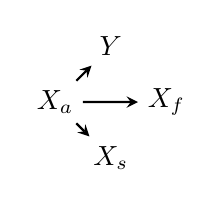
\begin{tikzpicture} [node distance = 1cm, on grid, auto, scale = 0.9]
\node (x1) {$X_a$};
\node (x2) [below right = of x1] {$X_s$};
\node (x3) [above right = of x2] {$X_f$};
\node (x4) [above right = of x1] {$Y$};
\path [-stealth, thick]
    (x1) edge [left] node {} (x2)
    (x1) edge [left] node {} (x3)
    (x1) edge [left] node {} (x4);
\end{tikzpicture}
\quad
b)
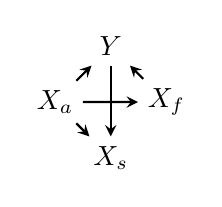
\begin{tikzpicture} [node distance = 1cm, on grid, auto, scale = 0.9]
\node (x1) {$X_a$};
\node (x2) [below right = of x1] {$X_s$};
\node (x3) [above right = of x2] {$X_f$};
\node (x4) [above right = of x1] {$Y$};
\path [-stealth, thick]
    (x1) edge [left] node {} (x2)
    (x1) edge [left] node {} (x3)
    (x1) edge [left] node {} (x4)
    (x4) edge [left] node {} (x2)
    (x3) edge [left] node {} (x4);
\end{tikzpicture}
\quad
c)
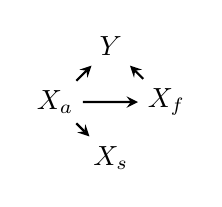
\begin{tikzpicture} [node distance = 1cm, on grid, auto, scale = 0.9]
\node (x1) {$X_a$};
\node (x2) [below right = of x1] {$X_s$};
\node (x3) [above right = of x2] {$X_f$};
\node (x4) [above right = of x1] {$Y$};
\path [-stealth, thick]
    (x1) edge [left] node {} (x2)
    (x1) edge [left] node {} (x3)
    (x1) edge [left] node {} (x4)
    (x3) edge [left] node {} (x4);
\end{tikzpicture}
\caption{Three plausible Bayesian Networks for the `Cohort II' data set.}
\label{bayesnets}
\end{figure}
The graphical represntaion allows us to directlyread off the conditional independence assumptions from the DAGs in Fig~\ref{bayesnets}. For example, in a) we have that $Y \ind X_f, X_s \ | \ X_a$ and that the factorisation of the joint probability mass function of $(X_a, X_s, X_f, Y)$ is given by:
\[p(x_a, x_s, x_f, y) = p(x_a)p(x_s|x_a)p(x_f|x_a)p(y|x_a)\]
In b) we have that $X_s \ind X_f \ | \ X_a, Y$ and the mass function with ordering $(X_a, X_f, Y, X_s)$ factorises as:
\[p(x_a, x_s, x_f, y) = p(x_a)p(x_f|x_a)p(y|x_a, x_f)p(x_s|x_a, y)\]
Observe that the ordering $(X_a, X_f, Y, X_s)$ in a) would give the same graph and the same factorisation of $p(x_a, x_s, x_f, y)$. We cannot necessarily read a unique ordering from a DAG of a BN but all such orderings must correspond to the same factorisation.
Finally in c) we have that $Y \ind X_s \ | \ X_a$ and but contrary to the DAG in a) $Y \notind X_f\ | \ X_a$. A possible ordering of the variables in c) is $(X_a, X_s, X_f, Y)$ with the joint probability mass function factorising as:
\[p(x_a, x_s, x_f, y) = p(x_a)p(x_s|x_a)p(x_f|x_a)p(y|x_a, x_f)\]

It is now clear how Bayesian network representation can clearly encodes some conditional independence statements of the model. More conditional independence statements can be inferred from the graph using a d-separation property, the formal definition of which can be found in \cite{}
However, in certain cases the BN does not provide a rich enough structure to incorporate all information obtainable from the data set. This is the case, for example, when the conditional independence statements of the problem are asymmetric. In our example, we might want to encdoe the following assumption that $Y \ind X_s\ | \ X_f = \text{Everyday}$ but $Y \notind X_s\ | \ X_f = \text{4-6 days per week}$. Asymmetric assumption of this kind cannot be represented simply by the directed edges between variables in the BN. This motivates introduction of a new class of graphical models. 

\section{Chain Event Graphs}\label{sec:cegs}
\emph{Chain Event Graphs} are a family of graphical statistical models derived from well-known probability trees. Their interpretation is quite different from that of a BNs introduced in the previous section: in particular, in the event-tree framework, vertices always correspond to events in an underlying probability space and not to random variables. Every edge $e = (v, v')$ depicts the possibility of transitioning from the donating vertex $v$ to the receiving vertex $v'$ and can be labelled by a corresponding transition probability $\theta(e)$. This is in contrast to the Bayesian Network where edges represent certain dependencies between the donating and receiving variables. \\
By introducing the concepts of \emph{stages} and \emph{positions} which group the vertices of a tree according to their associated conditional probabilities, an event tree becomes a \emph{staged tree}. The tree structure is then tightened by transforming it into a new, more compact object called a \emph{Chain Event Graph (CEG)}. In this section we define these concepts and support them with illustrative examples based on the 'Cohort II' Study from Section~\ref{sec:cohortii}. We adopt the notation as introduced in \cite{smith2017cegs}. 

\subsection{Tree based models on the example of `Cohort II' study}\label{subsec:treemodels}

A finite graph denoted as a pair $\mathcal{T} = (V,E)$ with vertex set $V$ and edge set $E \subseteq V \times V$ is called a \emph{tree}, if it is connected and has no cycles. We call the set of vertices $\text{pa}(v) = \{v' \ | \ \text{there is } (v',v) \in E\}$ the \emph{parents} of $v \in V$ and $\text{ch}(v)=\{v' \in V \ | \ \text{there is } (v,v') \in E\}$ the set of \emph{children} of $v \in V$. A vertex without parents is called a \emph{root} of the tree, usually denoted $v_0 \in V$, and vertices without children are called \emph{leaves}. Non-leaves, or inner vertices, are also called \emph{situations}. We call a pair $\mathcal{F}(v) = (v,E(v))$ of a vertex $v \in V$ together with its emanating edges $E(v) = \{(v,v') \in E \ | \ v' \in \text{ch}(v)\}$ a \emph{floret}.
\begin{definition}[Probability tree]
Let $\mathcal{T} = (V, E)$ be an event tree with parameters $\theta(e) = \theta(v, v')$ associated to all edges $e = (v, v') \in E$. We call the vector $\boldsymbol{\theta}_v = (\theta(e)| e \in E(v))$ of all parameters associated to the same floret a vector of floret parameters. If all labels are strictly positive probabilities and the components of all floret parameter vectors sum to unity, so  $\theta(e) \in (0,1)$ and $\sum_{e \in E(v)}\theta(e) = 1$ for all $e \in E$ and all non-leaves $v \in V$, then the pair
$(\mathcal{T}, \boldsymbol{\theta}_{\mathcal{T}})$ of graph $\mathcal{T}$ and vector of all labels $\boldsymbol{\theta}_{\mathcal{T}} = (\theta(e)| e \in E))$ is called a probability tree.
\end{definition}
Tree-based models are especially useful where there exist a natural ordering of the variables of interest. In our example we want to gain knowledge about the influence of $X_a, X_s, X_f$ on the target variable $Y$. For this reason we would want $Y$ to be the last variable in the tree. The order of the other three variables is less obvious. We decide on the ordering $\boldsymbol{X} = (X_a, X_s, X_f, Y)$ which is supported by both BNs a) and c) in Fig~\ref{bayesnets}. 
Fig~\ref{eventtree} illustrates an event tree defined on $\boldsymbol{X}$. To every node $v$ of this tree we can attach a floret parameter vector $\boldsymbol{\theta}_v$ thought of as a vector of conditional transition probabilities emanating from that situation. For instance, $\boldsymbol{\theta}_{v_{25}} = (0.935, 0.065)$ means that male drivers who passed their test after the age of 21 and reported to drive their car daily are estimated to have 6.5\% chances of being involved in at least one accident during their first 6 months after passing the test. 
\begin{figure}
\centering

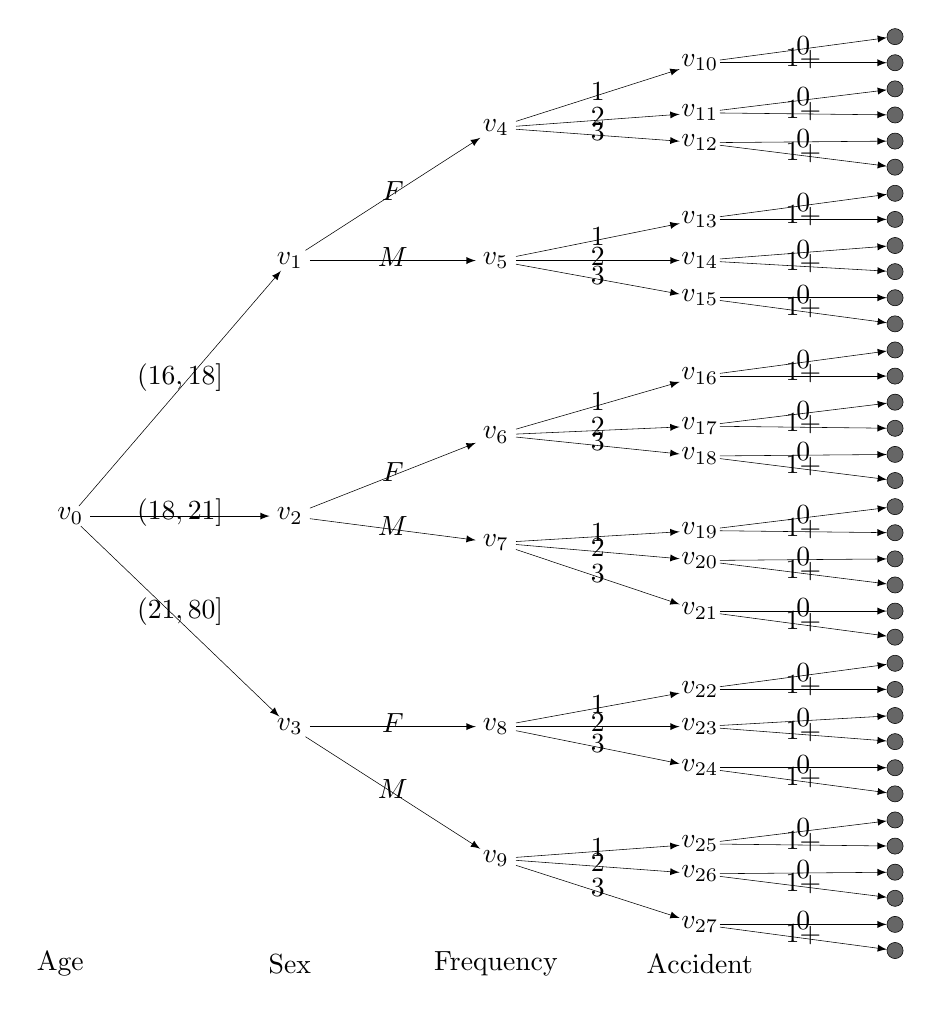
\begin{tikzpicture}[>=latex,line join=bevel, scale=0.2]
  \pgfsetlinewidth{0.2bp}
%%
\pgfsetcolor{black}
  % Edge: v_{0} -> v_{1}
  \draw [->] (51.484bp,814.53bp) .. controls (112.5bp,885.59bp) and (336.46bp,1146.4bp)  .. (415.19bp,1238.1bp);
  \definecolor{strokecol}{rgb}{0.0,0.0,0.0};
  \pgfsetstrokecolor{strokecol}
  \draw (233.5bp,1046.0bp) node {$(16,18]$};
  % Edge: v_{0} -> v_{2}
  \pgfsetcolor{black}
  \draw [->] (72.101bp,796.5bp) .. controls (144.0bp,796.5bp) and (305.02bp,796.5bp)  .. (394.84bp,796.5bp);
  \definecolor{strokecol}{rgb}{0.0,0.0,0.0};
  \pgfsetstrokecolor{strokecol}
  \draw (233.5bp,803.0bp) node {$(18,21]$};
  % Edge: v_{0} -> v_{3}
  \pgfsetcolor{black}
  \draw [->] (54.786bp,778.48bp) .. controls (118.99bp,716.87bp) and (329.82bp,514.58bp)  .. (412.1bp,435.64bp);
  \definecolor{strokecol}{rgb}{0.0,0.0,0.0};
  \pgfsetstrokecolor{strokecol}
  \draw (233.5bp,624.0bp) node {$(21,80]$};
  % Edge: v_{1} -> v_{4}
  \pgfsetcolor{black}
  \draw [->] (459.19bp,1274.7bp) .. controls (525.49bp,1317.4bp) and (691.26bp,1424.2bp)  .. (773.85bp,1477.4bp);
  \definecolor{strokecol}{rgb}{0.0,0.0,0.0};
  \pgfsetstrokecolor{strokecol}
  \draw (616.5bp,1382.0bp) node {$F$};
  % Edge: v_{1} -> v_{5}
  \pgfsetcolor{black}
  \draw [->] (467.25bp,1256.5bp) .. controls (535.08bp,1256.5bp) and (681.06bp,1256.5bp)  .. (765.88bp,1256.5bp);
  \definecolor{strokecol}{rgb}{0.0,0.0,0.0};
  \pgfsetstrokecolor{strokecol}
  \draw (616.5bp,1263.0bp) node {$M$};
  % Edge: v_{2} -> v_{6}
  \pgfsetcolor{black}
  \draw [->] (467.25bp,810.76bp) .. controls (535.21bp,837.51bp) and (681.65bp,895.14bp)  .. (765.88bp,928.28bp);
  \definecolor{strokecol}{rgb}{0.0,0.0,0.0};
  \pgfsetstrokecolor{strokecol}
  \draw (616.5bp,876.0bp) node {$F$};
  % Edge: v_{2} -> v_{7}
  \pgfsetcolor{black}
  \draw [->] (467.25bp,791.81bp) .. controls (535.08bp,783.03bp) and (681.06bp,764.15bp)  .. (765.88bp,753.17bp);
  \definecolor{strokecol}{rgb}{0.0,0.0,0.0};
  \pgfsetstrokecolor{strokecol}
  \draw (616.5bp,779.0bp) node {$M$};
  % Edge: v_{3} -> v_{8}
  \pgfsetcolor{black}
  \draw [->] (467.25bp,417.5bp) .. controls (535.08bp,417.5bp) and (681.06bp,417.5bp)  .. (765.88bp,417.5bp);
  \definecolor{strokecol}{rgb}{0.0,0.0,0.0};
  \pgfsetstrokecolor{strokecol}
  \draw (616.5bp,424.0bp) node {$F$};
  % Edge: v_{3} -> v_{9}
  \pgfsetcolor{black}
  \draw [->] (459.19bp,399.42bp) .. controls (525.49bp,356.89bp) and (691.26bp,250.54bp)  .. (773.85bp,197.56bp);
  \definecolor{strokecol}{rgb}{0.0,0.0,0.0};
  \pgfsetstrokecolor{strokecol}
  \draw (616.5bp,305.0bp) node {$M$};
  % Edge: v_{4} -> v_{10}
  \pgfsetcolor{black}
  \draw [->] (838.19bp,1507.0bp) .. controls (905.29bp,1528.4bp) and (1048.9bp,1574.2bp)  .. (1132.8bp,1601.0bp);
  \definecolor{strokecol}{rgb}{0.0,0.0,0.0};
  \pgfsetstrokecolor{strokecol}
  \draw (985.5bp,1560.0bp) node {$1$};
  % Edge: v_{4} -> v_{11}
  \pgfsetcolor{black}
  \draw [->] (838.19bp,1498.2bp) .. controls (905.16bp,1503.1bp) and (1048.3bp,1513.6bp)  .. (1132.8bp,1519.8bp);
  \definecolor{strokecol}{rgb}{0.0,0.0,0.0};
  \pgfsetstrokecolor{strokecol}
  \draw (985.5bp,1515.0bp) node {$2$};
  % Edge: v_{4} -> v_{12}
  \pgfsetcolor{black}
  \draw [->] (838.19bp,1492.8bp) .. controls (905.16bp,1487.9bp) and (1048.3bp,1477.4bp)  .. (1132.8bp,1471.2bp);
  \definecolor{strokecol}{rgb}{0.0,0.0,0.0};
  \pgfsetstrokecolor{strokecol}
  \draw (985.5bp,1488.0bp) node {$3$};
  % Edge: v_{5} -> v_{13}
  \pgfsetcolor{black}
  \draw [->] (838.19bp,1263.8bp) .. controls (905.29bp,1277.3bp) and (1048.9bp,1306.3bp)  .. (1132.8bp,1323.2bp);
  \definecolor{strokecol}{rgb}{0.0,0.0,0.0};
  \pgfsetstrokecolor{strokecol}
  \draw (985.5bp,1300.0bp) node {$1$};
  % Edge: v_{5} -> v_{14}
  \pgfsetcolor{black}
  \draw [->] (838.19bp,1256.5bp) .. controls (905.16bp,1256.5bp) and (1048.3bp,1256.5bp)  .. (1132.8bp,1256.5bp);
  \definecolor{strokecol}{rgb}{0.0,0.0,0.0};
  \pgfsetstrokecolor{strokecol}
  \draw (985.5bp,1263.0bp) node {$2$};
  % Edge: v_{5} -> v_{15}
  \pgfsetcolor{black}
  \draw [->] (838.19bp,1249.9bp) .. controls (905.29bp,1237.6bp) and (1048.9bp,1211.4bp)  .. (1132.8bp,1196.1bp);
  \definecolor{strokecol}{rgb}{0.0,0.0,0.0};
  \pgfsetstrokecolor{strokecol}
  \draw (985.5bp,1229.0bp) node {$3$};
  % Edge: v_{6} -> v_{16}
  \pgfsetcolor{black}
  \draw [->] (838.19bp,952.95bp) .. controls (905.29bp,972.33bp) and (1048.9bp,1013.8bp)  .. (1132.8bp,1038.0bp);
  \definecolor{strokecol}{rgb}{0.0,0.0,0.0};
  \pgfsetstrokecolor{strokecol}
  \draw (985.5bp,1002.0bp) node {$1$};
  % Edge: v_{6} -> v_{17}
  \pgfsetcolor{black}
  \draw [->] (838.19bp,944.08bp) .. controls (905.16bp,947.0bp) and (1048.3bp,953.24bp)  .. (1132.8bp,956.92bp);
  \definecolor{strokecol}{rgb}{0.0,0.0,0.0};
  \pgfsetstrokecolor{strokecol}
  \draw (985.5bp,957.0bp) node {$2$};
  % Edge: v_{6} -> v_{18}
  \pgfsetcolor{black}
  \draw [->] (838.19bp,938.75bp) .. controls (905.29bp,931.8bp) and (1048.9bp,916.94bp)  .. (1132.8bp,908.25bp);
  \definecolor{strokecol}{rgb}{0.0,0.0,0.0};
  \pgfsetstrokecolor{strokecol}
  \draw (985.5bp,930.0bp) node {$3$};
  % Edge: v_{7} -> v_{19}
  \pgfsetcolor{black}
  \draw [->] (838.19bp,750.67bp) .. controls (905.16bp,754.68bp) and (1048.3bp,763.26bp)  .. (1132.8bp,768.33bp);
  \definecolor{strokecol}{rgb}{0.0,0.0,0.0};
  \pgfsetstrokecolor{strokecol}
  \draw (985.5bp,766.0bp) node {$1$};
  % Edge: v_{7} -> v_{20}
  \pgfsetcolor{black}
  \draw [->] (838.19bp,745.34bp) .. controls (905.16bp,739.51bp) and (1048.3bp,727.03bp)  .. (1132.8bp,719.66bp);
  \definecolor{strokecol}{rgb}{0.0,0.0,0.0};
  \pgfsetstrokecolor{strokecol}
  \draw (985.5bp,739.0bp) node {$2$};
  % Edge: v_{7} -> v_{21}
  \pgfsetcolor{black}
  \draw [->] (838.19bp,736.37bp) .. controls (905.43bp,713.84bp) and (1049.5bp,665.56bp)  .. (1132.8bp,637.63bp);
  \definecolor{strokecol}{rgb}{0.0,0.0,0.0};
  \pgfsetstrokecolor{strokecol}
  \draw (985.5bp,693.0bp) node {$3$};
  % Edge: v_{8} -> v_{22}
  \pgfsetcolor{black}
  \draw [->] (838.19bp,424.11bp) .. controls (905.29bp,436.36bp) and (1048.9bp,462.57bp)  .. (1132.8bp,477.89bp);
  \definecolor{strokecol}{rgb}{0.0,0.0,0.0};
  \pgfsetstrokecolor{strokecol}
  \draw (985.5bp,457.0bp) node {$1$};
  % Edge: v_{8} -> v_{23}
  \pgfsetcolor{black}
  \draw [->] (838.19bp,417.5bp) .. controls (905.16bp,417.5bp) and (1048.3bp,417.5bp)  .. (1132.8bp,417.5bp);
  \definecolor{strokecol}{rgb}{0.0,0.0,0.0};
  \pgfsetstrokecolor{strokecol}
  \draw (985.5bp,424.0bp) node {$2$};
  % Edge: v_{8} -> v_{24}
  \pgfsetcolor{black}
  \draw [->] (838.19bp,410.2bp) .. controls (905.29bp,396.67bp) and (1048.9bp,367.72bp)  .. (1132.8bp,350.8bp);
  \definecolor{strokecol}{rgb}{0.0,0.0,0.0};
  \pgfsetstrokecolor{strokecol}
  \draw (985.5bp,387.0bp) node {$3$};
  % Edge: v_{9} -> v_{25}
  \pgfsetcolor{black}
  \draw [->] (838.19bp,182.16bp) .. controls (905.16bp,187.09bp) and (1048.3bp,197.62bp)  .. (1132.8bp,203.84bp);
  \definecolor{strokecol}{rgb}{0.0,0.0,0.0};
  \pgfsetstrokecolor{strokecol}
  \draw (985.5bp,199.0bp) node {$1$};
  % Edge: v_{9} -> v_{26}
  \pgfsetcolor{black}
  \draw [->] (838.19bp,176.84bp) .. controls (905.16bp,171.91bp) and (1048.3bp,161.38bp)  .. (1132.8bp,155.16bp);
  \definecolor{strokecol}{rgb}{0.0,0.0,0.0};
  \pgfsetstrokecolor{strokecol}
  \draw (985.5bp,172.0bp) node {$2$};
  % Edge: v_{9} -> v_{27}
  \pgfsetcolor{black}
  \draw [->] (838.19bp,167.86bp) .. controls (905.29bp,146.29bp) and (1048.9bp,100.12bp)  .. (1132.8bp,73.137bp);
  \definecolor{strokecol}{rgb}{0.0,0.0,0.0};
  \pgfsetstrokecolor{strokecol}
  \draw (985.5bp,127.0bp) node {$3$};
  % Edge: v_{10} -> v_{28}
  \pgfsetcolor{black}
  \draw [->] (1205.3bp,1617.4bp) .. controls (1277.0bp,1626.9bp) and (1435.0bp,1648.1bp)  .. (1506.1bp,1657.6bp);
  \definecolor{strokecol}{rgb}{0.0,0.0,0.0};
  \pgfsetstrokecolor{strokecol}
  \draw (1355.5bp,1643.0bp) node {$0$};
  % Edge: v_{10} -> v_{29}
  \pgfsetcolor{black}
  \draw [->] (1205.3bp,1612.5bp) .. controls (1276.8bp,1612.5bp) and (1434.2bp,1612.5bp)  .. (1505.7bp,1612.5bp);
  \definecolor{strokecol}{rgb}{0.0,0.0,0.0};
  \pgfsetstrokecolor{strokecol}
  \draw (1355.5bp,1619.0bp) node {$1+$};
  % Edge: v_{11} -> v_{30}
  \pgfsetcolor{black}
  \draw [->] (1205.3bp,1526.9bp) .. controls (1277.0bp,1535.7bp) and (1435.0bp,1555.0bp)  .. (1506.1bp,1563.7bp);
  \definecolor{strokecol}{rgb}{0.0,0.0,0.0};
  \pgfsetstrokecolor{strokecol}
  \draw (1355.5bp,1551.0bp) node {$0$};
  % Edge: v_{11} -> v_{31}
  \pgfsetcolor{black}
  \draw [->] (1205.3bp,1522.1bp) .. controls (1276.8bp,1521.3bp) and (1434.2bp,1519.5bp)  .. (1505.7bp,1518.7bp);
  \definecolor{strokecol}{rgb}{0.0,0.0,0.0};
  \pgfsetstrokecolor{strokecol}
  \draw (1355.5bp,1526.0bp) node {$1+$};
  % Edge: v_{12} -> v_{32}
  \pgfsetcolor{black}
  \draw [->] (1205.3bp,1468.8bp) .. controls (1276.8bp,1469.4bp) and (1434.2bp,1470.8bp)  .. (1505.7bp,1471.4bp);
  \definecolor{strokecol}{rgb}{0.0,0.0,0.0};
  \pgfsetstrokecolor{strokecol}
  \draw (1355.5bp,1476.0bp) node {$0$};
  % Edge: v_{12} -> v_{33}
  \pgfsetcolor{black}
  \draw [->] (1205.3bp,1464.0bp) .. controls (1277.0bp,1455.0bp) and (1435.0bp,1435.2bp)  .. (1506.1bp,1426.3bp);
  \definecolor{strokecol}{rgb}{0.0,0.0,0.0};
  \pgfsetstrokecolor{strokecol}
  \draw (1355.5bp,1451.0bp) node {$1+$};
  % Edge: v_{13} -> v_{34}
  \pgfsetcolor{black}
  \draw [->] (1205.3bp,1335.4bp) .. controls (1277.0bp,1344.9bp) and (1435.0bp,1366.1bp)  .. (1506.1bp,1375.6bp);
  \definecolor{strokecol}{rgb}{0.0,0.0,0.0};
  \pgfsetstrokecolor{strokecol}
  \draw (1355.5bp,1361.0bp) node {$0$};
  % Edge: v_{13} -> v_{35}
  \pgfsetcolor{black}
  \draw [->] (1205.3bp,1330.5bp) .. controls (1276.8bp,1330.5bp) and (1434.2bp,1330.5bp)  .. (1505.7bp,1330.5bp);
  \definecolor{strokecol}{rgb}{0.0,0.0,0.0};
  \pgfsetstrokecolor{strokecol}
  \draw (1355.5bp,1337.0bp) node {$1+$};
  % Edge: v_{14} -> v_{36}
  \pgfsetcolor{black}
  \draw [->] (1205.3bp,1259.3bp) .. controls (1276.8bp,1264.8bp) and (1434.2bp,1276.9bp)  .. (1505.7bp,1282.4bp);
  \definecolor{strokecol}{rgb}{0.0,0.0,0.0};
  \pgfsetstrokecolor{strokecol}
  \draw (1355.5bp,1277.0bp) node {$0$};
  % Edge: v_{14} -> v_{37}
  \pgfsetcolor{black}
  \draw [->] (1205.3bp,1254.4bp) .. controls (1276.8bp,1250.4bp) and (1434.2bp,1241.4bp)  .. (1505.7bp,1237.3bp);
  \definecolor{strokecol}{rgb}{0.0,0.0,0.0};
  \pgfsetstrokecolor{strokecol}
  \draw (1355.5bp,1252.0bp) node {$1+$};
  % Edge: v_{15} -> v_{38}
  \pgfsetcolor{black}
  \draw [->] (1205.3bp,1189.5bp) .. controls (1276.8bp,1189.5bp) and (1434.2bp,1189.5bp)  .. (1505.7bp,1189.5bp);
  \definecolor{strokecol}{rgb}{0.0,0.0,0.0};
  \pgfsetstrokecolor{strokecol}
  \draw (1355.5bp,1196.0bp) node {$0$};
  % Edge: v_{15} -> v_{39}
  \pgfsetcolor{black}
  \draw [->] (1205.3bp,1184.6bp) .. controls (1277.0bp,1175.1bp) and (1435.0bp,1153.9bp)  .. (1506.1bp,1144.4bp);
  \definecolor{strokecol}{rgb}{0.0,0.0,0.0};
  \pgfsetstrokecolor{strokecol}
  \draw (1355.5bp,1171.0bp) node {$1+$};
  % Edge: v_{16} -> v_{40}
  \pgfsetcolor{black}
  \draw [->] (1205.3bp,1053.4bp) .. controls (1277.0bp,1062.9bp) and (1435.0bp,1084.1bp)  .. (1506.1bp,1093.6bp);
  \definecolor{strokecol}{rgb}{0.0,0.0,0.0};
  \pgfsetstrokecolor{strokecol}
  \draw (1355.5bp,1079.0bp) node {$0$};
  % Edge: v_{16} -> v_{41}
  \pgfsetcolor{black}
  \draw [->] (1205.3bp,1048.5bp) .. controls (1276.8bp,1048.5bp) and (1434.2bp,1048.5bp)  .. (1505.7bp,1048.5bp);
  \definecolor{strokecol}{rgb}{0.0,0.0,0.0};
  \pgfsetstrokecolor{strokecol}
  \draw (1355.5bp,1055.0bp) node {$1+$};
  % Edge: v_{17} -> v_{42}
  \pgfsetcolor{black}
  \draw [->] (1205.3bp,962.94bp) .. controls (1277.0bp,971.71bp) and (1435.0bp,991.04bp)  .. (1506.1bp,999.74bp);
  \definecolor{strokecol}{rgb}{0.0,0.0,0.0};
  \pgfsetstrokecolor{strokecol}
  \draw (1355.5bp,987.0bp) node {$0$};
  % Edge: v_{17} -> v_{43}
  \pgfsetcolor{black}
  \draw [->] (1205.3bp,958.09bp) .. controls (1276.8bp,957.27bp) and (1434.2bp,955.48bp)  .. (1505.7bp,954.67bp);
  \definecolor{strokecol}{rgb}{0.0,0.0,0.0};
  \pgfsetstrokecolor{strokecol}
  \draw (1355.5bp,962.0bp) node {$1+$};
  % Edge: v_{18} -> v_{44}
  \pgfsetcolor{black}
  \draw [->] (1205.3bp,904.81bp) .. controls (1276.8bp,905.42bp) and (1434.2bp,906.76bp)  .. (1505.7bp,907.37bp);
  \definecolor{strokecol}{rgb}{0.0,0.0,0.0};
  \pgfsetstrokecolor{strokecol}
  \draw (1355.5bp,912.0bp) node {$0$};
  % Edge: v_{18} -> v_{45}
  \pgfsetcolor{black}
  \draw [->] (1205.3bp,899.96bp) .. controls (1277.0bp,890.99bp) and (1435.0bp,871.21bp)  .. (1506.1bp,862.3bp);
  \definecolor{strokecol}{rgb}{0.0,0.0,0.0};
  \pgfsetstrokecolor{strokecol}
  \draw (1355.5bp,887.0bp) node {$1+$};
  % Edge: v_{19} -> v_{46}
  \pgfsetcolor{black}
  \draw [->] (1205.3bp,774.94bp) .. controls (1277.0bp,783.71bp) and (1435.0bp,803.04bp)  .. (1506.1bp,811.74bp);
  \definecolor{strokecol}{rgb}{0.0,0.0,0.0};
  \pgfsetstrokecolor{strokecol}
  \draw (1355.5bp,799.0bp) node {$0$};
  % Edge: v_{19} -> v_{47}
  \pgfsetcolor{black}
  \draw [->] (1205.3bp,770.09bp) .. controls (1276.8bp,769.27bp) and (1434.2bp,767.48bp)  .. (1505.7bp,766.67bp);
  \definecolor{strokecol}{rgb}{0.0,0.0,0.0};
  \pgfsetstrokecolor{strokecol}
  \draw (1355.5bp,774.0bp) node {$1+$};
  % Edge: v_{20} -> v_{48}
  \pgfsetcolor{black}
  \draw [->] (1205.3bp,716.81bp) .. controls (1276.8bp,717.42bp) and (1434.2bp,718.76bp)  .. (1505.7bp,719.37bp);
  \definecolor{strokecol}{rgb}{0.0,0.0,0.0};
  \pgfsetstrokecolor{strokecol}
  \draw (1355.5bp,724.0bp) node {$0$};
  % Edge: v_{20} -> v_{49}
  \pgfsetcolor{black}
  \draw [->] (1205.3bp,711.96bp) .. controls (1277.0bp,702.99bp) and (1435.0bp,683.21bp)  .. (1506.1bp,674.3bp);
  \definecolor{strokecol}{rgb}{0.0,0.0,0.0};
  \pgfsetstrokecolor{strokecol}
  \draw (1355.5bp,699.0bp) node {$1+$};
  % Edge: v_{21} -> v_{50}
  \pgfsetcolor{black}
  \draw [->] (1205.3bp,625.5bp) .. controls (1276.8bp,625.5bp) and (1434.2bp,625.5bp)  .. (1505.7bp,625.5bp);
  \definecolor{strokecol}{rgb}{0.0,0.0,0.0};
  \pgfsetstrokecolor{strokecol}
  \draw (1355.5bp,632.0bp) node {$0$};
  % Edge: v_{21} -> v_{51}
  \pgfsetcolor{black}
  \draw [->] (1205.3bp,620.65bp) .. controls (1277.0bp,611.06bp) and (1435.0bp,589.94bp)  .. (1506.1bp,580.43bp);
  \definecolor{strokecol}{rgb}{0.0,0.0,0.0};
  \pgfsetstrokecolor{strokecol}
  \draw (1355.5bp,607.0bp) node {$1+$};
  % Edge: v_{22} -> v_{52}
  \pgfsetcolor{black}
  \draw [->] (1205.3bp,489.35bp) .. controls (1277.0bp,498.94bp) and (1435.0bp,520.06bp)  .. (1506.1bp,529.57bp);
  \definecolor{strokecol}{rgb}{0.0,0.0,0.0};
  \pgfsetstrokecolor{strokecol}
  \draw (1355.5bp,515.0bp) node {$0$};
  % Edge: v_{22} -> v_{53}
  \pgfsetcolor{black}
  \draw [->] (1205.3bp,484.5bp) .. controls (1276.8bp,484.5bp) and (1434.2bp,484.5bp)  .. (1505.7bp,484.5bp);
  \definecolor{strokecol}{rgb}{0.0,0.0,0.0};
  \pgfsetstrokecolor{strokecol}
  \draw (1355.5bp,491.0bp) node {$1+$};
  % Edge: v_{23} -> v_{54}
  \pgfsetcolor{black}
  \draw [->] (1205.3bp,419.57bp) .. controls (1276.8bp,423.63bp) and (1434.2bp,432.59bp)  .. (1505.7bp,436.66bp);
  \definecolor{strokecol}{rgb}{0.0,0.0,0.0};
  \pgfsetstrokecolor{strokecol}
  \draw (1355.5bp,434.0bp) node {$0$};
  % Edge: v_{23} -> v_{55}
  \pgfsetcolor{black}
  \draw [->] (1205.3bp,414.71bp) .. controls (1276.8bp,409.22bp) and (1434.2bp,397.13bp)  .. (1505.7bp,391.63bp);
  \definecolor{strokecol}{rgb}{0.0,0.0,0.0};
  \pgfsetstrokecolor{strokecol}
  \draw (1355.5bp,409.0bp) node {$1+$};
  % Edge: v_{24} -> v_{56}
  \pgfsetcolor{black}
  \draw [->] (1205.3bp,343.5bp) .. controls (1276.8bp,343.5bp) and (1434.2bp,343.5bp)  .. (1505.7bp,343.5bp);
  \definecolor{strokecol}{rgb}{0.0,0.0,0.0};
  \pgfsetstrokecolor{strokecol}
  \draw (1355.5bp,350.0bp) node {$0$};
  % Edge: v_{24} -> v_{57}
  \pgfsetcolor{black}
  \draw [->] (1205.3bp,338.65bp) .. controls (1277.0bp,329.06bp) and (1435.0bp,307.94bp)  .. (1506.1bp,298.43bp);
  \definecolor{strokecol}{rgb}{0.0,0.0,0.0};
  \pgfsetstrokecolor{strokecol}
  \draw (1355.5bp,325.0bp) node {$1+$};
  % Edge: v_{25} -> v_{58}
  \pgfsetcolor{black}
  \draw [->] (1205.3bp,210.94bp) .. controls (1277.0bp,219.71bp) and (1435.0bp,239.04bp)  .. (1506.1bp,247.74bp);
  \definecolor{strokecol}{rgb}{0.0,0.0,0.0};
  \pgfsetstrokecolor{strokecol}
  \draw (1355.5bp,235.0bp) node {$0$};
  % Edge: v_{25} -> v_{59}
  \pgfsetcolor{black}
  \draw [->] (1205.3bp,206.09bp) .. controls (1276.8bp,205.27bp) and (1434.2bp,203.48bp)  .. (1505.7bp,202.67bp);
  \definecolor{strokecol}{rgb}{0.0,0.0,0.0};
  \pgfsetstrokecolor{strokecol}
  \draw (1355.5bp,210.0bp) node {$1+$};
  % Edge: v_{26} -> v_{60}
  \pgfsetcolor{black}
  \draw [->] (1205.3bp,152.81bp) .. controls (1276.8bp,153.42bp) and (1434.2bp,154.76bp)  .. (1505.7bp,155.37bp);
  \definecolor{strokecol}{rgb}{0.0,0.0,0.0};
  \pgfsetstrokecolor{strokecol}
  \draw (1355.5bp,160.0bp) node {$0$};
  % Edge: v_{26} -> v_{61}
  \pgfsetcolor{black}
  \draw [->] (1205.3bp,147.96bp) .. controls (1277.0bp,138.99bp) and (1435.0bp,119.21bp)  .. (1506.1bp,110.3bp);
  \definecolor{strokecol}{rgb}{0.0,0.0,0.0};
  \pgfsetstrokecolor{strokecol}
  \draw (1355.5bp,135.0bp) node {$1+$};
  % Edge: v_{27} -> v_{62}
  \pgfsetcolor{black}
  \draw [->] (1205.3bp,61.5bp) .. controls (1276.8bp,61.5bp) and (1434.2bp,61.5bp)  .. (1505.7bp,61.5bp);
  \definecolor{strokecol}{rgb}{0.0,0.0,0.0};
  \pgfsetstrokecolor{strokecol}
  \draw (1355.5bp,68.0bp) node {$0$};
  % Edge: v_{27} -> v_{63}
  \pgfsetcolor{black}
  \draw [->] (1205.3bp,56.647bp) .. controls (1277.0bp,47.065bp) and (1435.0bp,25.937bp)  .. (1506.1bp,16.428bp);
  \definecolor{strokecol}{rgb}{0.0,0.0,0.0};
  \pgfsetstrokecolor{strokecol}
  \draw (1355.5bp,43.0bp) node {$1+$};
  % Node: v_{0}
\begin{scope}
  \definecolor{strokecol}{rgb}{0.0,0.0,0.0};
  \pgfsetstrokecolor{strokecol}
  \draw (36.0bp,796.5bp) node {$v_{0}$};
\end{scope}
  % Node: v_{1}
\begin{scope}
  \definecolor{strokecol}{rgb}{0.0,0.0,0.0};
  \pgfsetstrokecolor{strokecol}
  \draw (431.0bp,1256.5bp) node {$v_{1}$};
\end{scope}
  % Node: v_{2}
\begin{scope}
  \definecolor{strokecol}{rgb}{0.0,0.0,0.0};
  \pgfsetstrokecolor{strokecol}
  \draw (431.0bp,796.5bp) node {$v_{2}$};
\end{scope}
  % Node: v_{3}
\begin{scope}
  \definecolor{strokecol}{rgb}{0.0,0.0,0.0};
  \pgfsetstrokecolor{strokecol}
  \draw (431.0bp,417.5bp) node {$v_{3}$};
\end{scope}
  % Node: v_{4}
\begin{scope}
  \definecolor{strokecol}{rgb}{0.0,0.0,0.0};
  \pgfsetstrokecolor{strokecol}
  \draw (802.0bp,1495.5bp) node {$v_{4}$};
\end{scope}
  % Node: v_{5}
\begin{scope}
  \definecolor{strokecol}{rgb}{0.0,0.0,0.0};
  \pgfsetstrokecolor{strokecol}
  \draw (802.0bp,1256.5bp) node {$v_{5}$};
\end{scope}
  % Node: v_{6}
\begin{scope}
  \definecolor{strokecol}{rgb}{0.0,0.0,0.0};
  \pgfsetstrokecolor{strokecol}
  \draw (802.0bp,942.5bp) node {$v_{6}$};
\end{scope}
  % Node: v_{7}
\begin{scope}
  \definecolor{strokecol}{rgb}{0.0,0.0,0.0};
  \pgfsetstrokecolor{strokecol}
  \draw (802.0bp,748.5bp) node {$v_{7}$};
\end{scope}
  % Node: v_{8}
\begin{scope}
  \definecolor{strokecol}{rgb}{0.0,0.0,0.0};
  \pgfsetstrokecolor{strokecol}
  \draw (802.0bp,417.5bp) node {$v_{8}$};
\end{scope}
  % Node: v_{9}
\begin{scope}
  \definecolor{strokecol}{rgb}{0.0,0.0,0.0};
  \pgfsetstrokecolor{strokecol}
  \draw (802.0bp,179.5bp) node {$v_{9}$};
\end{scope}
  % Node: v_{10}
\begin{scope}
  \definecolor{strokecol}{rgb}{0.0,0.0,0.0};
  \pgfsetstrokecolor{strokecol}
  \draw (1169.0bp,1612.5bp) node {$v_{10}$};
\end{scope}
  % Node: v_{11}
\begin{scope}
  \definecolor{strokecol}{rgb}{0.0,0.0,0.0};
  \pgfsetstrokecolor{strokecol}
  \draw (1169.0bp,1522.5bp) node {$v_{11}$};
\end{scope}
  % Node: v_{12}
\begin{scope}
  \definecolor{strokecol}{rgb}{0.0,0.0,0.0};
  \pgfsetstrokecolor{strokecol}
  \draw (1169.0bp,1468.5bp) node {$v_{12}$};
\end{scope}
  % Node: v_{13}
\begin{scope}
  \definecolor{strokecol}{rgb}{0.0,0.0,0.0};
  \pgfsetstrokecolor{strokecol}
  \draw (1169.0bp,1330.5bp) node {$v_{13}$};
\end{scope}
  % Node: v_{14}
\begin{scope}
  \definecolor{strokecol}{rgb}{0.0,0.0,0.0};
  \pgfsetstrokecolor{strokecol}
  \draw (1169.0bp,1256.5bp) node {$v_{14}$};
\end{scope}
  % Node: v_{15}
\begin{scope}
  \definecolor{strokecol}{rgb}{0.0,0.0,0.0};
  \pgfsetstrokecolor{strokecol}
  \draw (1169.0bp,1189.5bp) node {$v_{15}$};
\end{scope}
  % Node: v_{16}
\begin{scope}
  \definecolor{strokecol}{rgb}{0.0,0.0,0.0};
  \pgfsetstrokecolor{strokecol}
  \draw (1169.0bp,1048.5bp) node {$v_{16}$};
\end{scope}
  % Node: v_{17}
\begin{scope}
  \definecolor{strokecol}{rgb}{0.0,0.0,0.0};
  \pgfsetstrokecolor{strokecol}
  \draw (1169.0bp,958.5bp) node {$v_{17}$};
\end{scope}
  % Node: v_{18}
\begin{scope}
  \definecolor{strokecol}{rgb}{0.0,0.0,0.0};
  \pgfsetstrokecolor{strokecol}
  \draw (1169.0bp,904.5bp) node {$v_{18}$};
\end{scope}
  % Node: v_{19}
\begin{scope}
  \definecolor{strokecol}{rgb}{0.0,0.0,0.0};
  \pgfsetstrokecolor{strokecol}
  \draw (1169.0bp,770.5bp) node {$v_{19}$};
\end{scope}
  % Node: v_{20}
\begin{scope}
  \definecolor{strokecol}{rgb}{0.0,0.0,0.0};
  \pgfsetstrokecolor{strokecol}
  \draw (1169.0bp,716.5bp) node {$v_{20}$};
\end{scope}
  % Node: v_{21}
\begin{scope}
  \definecolor{strokecol}{rgb}{0.0,0.0,0.0};
  \pgfsetstrokecolor{strokecol}
  \draw (1169.0bp,625.5bp) node {$v_{21}$};
\end{scope}
  % Node: v_{22}
\begin{scope}
  \definecolor{strokecol}{rgb}{0.0,0.0,0.0};
  \pgfsetstrokecolor{strokecol}
  \draw (1169.0bp,484.5bp) node {$v_{22}$};
\end{scope}
  % Node: v_{23}
\begin{scope}
  \definecolor{strokecol}{rgb}{0.0,0.0,0.0};
  \pgfsetstrokecolor{strokecol}
  \draw (1169.0bp,417.5bp) node {$v_{23}$};
\end{scope}
  % Node: v_{24}
\begin{scope}
  \definecolor{strokecol}{rgb}{0.0,0.0,0.0};
  \pgfsetstrokecolor{strokecol}
  \draw (1169.0bp,343.5bp) node {$v_{24}$};
\end{scope}
  % Node: v_{25}
\begin{scope}
  \definecolor{strokecol}{rgb}{0.0,0.0,0.0};
  \pgfsetstrokecolor{strokecol}
  \draw (1169.0bp,206.5bp) node {$v_{25}$};
\end{scope}
  % Node: v_{26}
\begin{scope}
  \definecolor{strokecol}{rgb}{0.0,0.0,0.0};
  \pgfsetstrokecolor{strokecol}
  \draw (1169.0bp,152.5bp) node {$v_{26}$};
\end{scope}
  % Node: v_{27}
\begin{scope}
  \definecolor{strokecol}{rgb}{0.0,0.0,0.0};
  \pgfsetstrokecolor{strokecol}
  \draw (1169.0bp,61.5bp) node {$v_{27}$};
\end{scope}
  % Node: v_{28}
\begin{scope}
  \definecolor{strokecol}{rgb}{0.0,0.0,0.0};
  \pgfsetstrokecolor{strokecol}
  \definecolor{fillcol}{rgb}{0.4,0.4,0.4};
  \pgfsetfillcolor{fillcol}
  \filldraw [opacity=1] (1520.5bp,1659.5bp) ellipse (14.5bp and 14.5bp);
\end{scope}
  % Node: v_{29}
\begin{scope}
  \definecolor{strokecol}{rgb}{0.0,0.0,0.0};
  \pgfsetstrokecolor{strokecol}
  \definecolor{fillcol}{rgb}{0.4,0.4,0.4};
  \pgfsetfillcolor{fillcol}
  \filldraw [opacity=1] (1520.5bp,1612.5bp) ellipse (14.5bp and 14.5bp);
\end{scope}
  % Node: v_{30}
\begin{scope}
  \definecolor{strokecol}{rgb}{0.0,0.0,0.0};
  \pgfsetstrokecolor{strokecol}
  \definecolor{fillcol}{rgb}{0.4,0.4,0.4};
  \pgfsetfillcolor{fillcol}
  \filldraw [opacity=1] (1520.5bp,1565.5bp) ellipse (14.5bp and 14.5bp);
\end{scope}
  % Node: v_{31}
\begin{scope}
  \definecolor{strokecol}{rgb}{0.0,0.0,0.0};
  \pgfsetstrokecolor{strokecol}
  \definecolor{fillcol}{rgb}{0.4,0.4,0.4};
  \pgfsetfillcolor{fillcol}
  \filldraw [opacity=1] (1520.5bp,1518.5bp) ellipse (14.5bp and 14.5bp);
\end{scope}
  % Node: v_{32}
\begin{scope}
  \definecolor{strokecol}{rgb}{0.0,0.0,0.0};
  \pgfsetstrokecolor{strokecol}
  \definecolor{fillcol}{rgb}{0.4,0.4,0.4};
  \pgfsetfillcolor{fillcol}
  \filldraw [opacity=1] (1520.5bp,1471.5bp) ellipse (14.5bp and 14.5bp);
\end{scope}
  % Node: v_{33}
\begin{scope}
  \definecolor{strokecol}{rgb}{0.0,0.0,0.0};
  \pgfsetstrokecolor{strokecol}
  \definecolor{fillcol}{rgb}{0.4,0.4,0.4};
  \pgfsetfillcolor{fillcol}
  \filldraw [opacity=1] (1520.5bp,1424.5bp) ellipse (14.5bp and 14.5bp);
\end{scope}
  % Node: v_{34}
\begin{scope}
  \definecolor{strokecol}{rgb}{0.0,0.0,0.0};
  \pgfsetstrokecolor{strokecol}
  \definecolor{fillcol}{rgb}{0.4,0.4,0.4};
  \pgfsetfillcolor{fillcol}
  \filldraw [opacity=1] (1520.5bp,1377.5bp) ellipse (14.5bp and 14.5bp);
\end{scope}
  % Node: v_{35}
\begin{scope}
  \definecolor{strokecol}{rgb}{0.0,0.0,0.0};
  \pgfsetstrokecolor{strokecol}
  \definecolor{fillcol}{rgb}{0.4,0.4,0.4};
  \pgfsetfillcolor{fillcol}
  \filldraw [opacity=1] (1520.5bp,1330.5bp) ellipse (14.5bp and 14.5bp);
\end{scope}
  % Node: v_{36}
\begin{scope}
  \definecolor{strokecol}{rgb}{0.0,0.0,0.0};
  \pgfsetstrokecolor{strokecol}
  \definecolor{fillcol}{rgb}{0.4,0.4,0.4};
  \pgfsetfillcolor{fillcol}
  \filldraw [opacity=1] (1520.5bp,1283.5bp) ellipse (14.5bp and 14.5bp);
\end{scope}
  % Node: v_{37}
\begin{scope}
  \definecolor{strokecol}{rgb}{0.0,0.0,0.0};
  \pgfsetstrokecolor{strokecol}
  \definecolor{fillcol}{rgb}{0.4,0.4,0.4};
  \pgfsetfillcolor{fillcol}
  \filldraw [opacity=1] (1520.5bp,1236.5bp) ellipse (14.5bp and 14.5bp);
\end{scope}
  % Node: v_{38}
\begin{scope}
  \definecolor{strokecol}{rgb}{0.0,0.0,0.0};
  \pgfsetstrokecolor{strokecol}
  \definecolor{fillcol}{rgb}{0.4,0.4,0.4};
  \pgfsetfillcolor{fillcol}
  \filldraw [opacity=1] (1520.5bp,1189.5bp) ellipse (14.5bp and 14.5bp);
\end{scope}
  % Node: v_{39}
\begin{scope}
  \definecolor{strokecol}{rgb}{0.0,0.0,0.0};
  \pgfsetstrokecolor{strokecol}
  \definecolor{fillcol}{rgb}{0.4,0.4,0.4};
  \pgfsetfillcolor{fillcol}
  \filldraw [opacity=1] (1520.5bp,1142.5bp) ellipse (14.5bp and 14.5bp);
\end{scope}
  % Node: v_{40}
\begin{scope}
  \definecolor{strokecol}{rgb}{0.0,0.0,0.0};
  \pgfsetstrokecolor{strokecol}
  \definecolor{fillcol}{rgb}{0.4,0.4,0.4};
  \pgfsetfillcolor{fillcol}
  \filldraw [opacity=1] (1520.5bp,1095.5bp) ellipse (14.5bp and 14.5bp);
\end{scope}
  % Node: v_{41}
\begin{scope}
  \definecolor{strokecol}{rgb}{0.0,0.0,0.0};
  \pgfsetstrokecolor{strokecol}
  \definecolor{fillcol}{rgb}{0.4,0.4,0.4};
  \pgfsetfillcolor{fillcol}
  \filldraw [opacity=1] (1520.5bp,1048.5bp) ellipse (14.5bp and 14.5bp);
\end{scope}
  % Node: v_{42}
\begin{scope}
  \definecolor{strokecol}{rgb}{0.0,0.0,0.0};
  \pgfsetstrokecolor{strokecol}
  \definecolor{fillcol}{rgb}{0.4,0.4,0.4};
  \pgfsetfillcolor{fillcol}
  \filldraw [opacity=1] (1520.5bp,1001.5bp) ellipse (14.5bp and 14.5bp);
\end{scope}
  % Node: v_{43}
\begin{scope}
  \definecolor{strokecol}{rgb}{0.0,0.0,0.0};
  \pgfsetstrokecolor{strokecol}
  \definecolor{fillcol}{rgb}{0.4,0.4,0.4};
  \pgfsetfillcolor{fillcol}
  \filldraw [opacity=1] (1520.5bp,954.5bp) ellipse (14.5bp and 14.5bp);
\end{scope}
  % Node: v_{44}
\begin{scope}
  \definecolor{strokecol}{rgb}{0.0,0.0,0.0};
  \pgfsetstrokecolor{strokecol}
  \definecolor{fillcol}{rgb}{0.4,0.4,0.4};
  \pgfsetfillcolor{fillcol}
  \filldraw [opacity=1] (1520.5bp,907.5bp) ellipse (14.5bp and 14.5bp);
\end{scope}
  % Node: v_{45}
\begin{scope}
  \definecolor{strokecol}{rgb}{0.0,0.0,0.0};
  \pgfsetstrokecolor{strokecol}
  \definecolor{fillcol}{rgb}{0.4,0.4,0.4};
  \pgfsetfillcolor{fillcol}
  \filldraw [opacity=1] (1520.5bp,860.5bp) ellipse (14.5bp and 14.5bp);
\end{scope}
  % Node: v_{46}
\begin{scope}
  \definecolor{strokecol}{rgb}{0.0,0.0,0.0};
  \pgfsetstrokecolor{strokecol}
  \definecolor{fillcol}{rgb}{0.4,0.4,0.4};
  \pgfsetfillcolor{fillcol}
  \filldraw [opacity=1] (1520.5bp,813.5bp) ellipse (14.5bp and 14.5bp);
\end{scope}
  % Node: v_{47}
\begin{scope}
  \definecolor{strokecol}{rgb}{0.0,0.0,0.0};
  \pgfsetstrokecolor{strokecol}
  \definecolor{fillcol}{rgb}{0.4,0.4,0.4};
  \pgfsetfillcolor{fillcol}
  \filldraw [opacity=1] (1520.5bp,766.5bp) ellipse (14.5bp and 14.5bp);
\end{scope}
  % Node: v_{48}
\begin{scope}
  \definecolor{strokecol}{rgb}{0.0,0.0,0.0};
  \pgfsetstrokecolor{strokecol}
  \definecolor{fillcol}{rgb}{0.4,0.4,0.4};
  \pgfsetfillcolor{fillcol}
  \filldraw [opacity=1] (1520.5bp,719.5bp) ellipse (14.5bp and 14.5bp);
\end{scope}
  % Node: v_{49}
\begin{scope}
  \definecolor{strokecol}{rgb}{0.0,0.0,0.0};
  \pgfsetstrokecolor{strokecol}
  \definecolor{fillcol}{rgb}{0.4,0.4,0.4};
  \pgfsetfillcolor{fillcol}
  \filldraw [opacity=1] (1520.5bp,672.5bp) ellipse (14.5bp and 14.5bp);
\end{scope}
  % Node: v_{50}
\begin{scope}
  \definecolor{strokecol}{rgb}{0.0,0.0,0.0};
  \pgfsetstrokecolor{strokecol}
  \definecolor{fillcol}{rgb}{0.4,0.4,0.4};
  \pgfsetfillcolor{fillcol}
  \filldraw [opacity=1] (1520.5bp,625.5bp) ellipse (14.5bp and 14.5bp);
\end{scope}
  % Node: v_{51}
\begin{scope}
  \definecolor{strokecol}{rgb}{0.0,0.0,0.0};
  \pgfsetstrokecolor{strokecol}
  \definecolor{fillcol}{rgb}{0.4,0.4,0.4};
  \pgfsetfillcolor{fillcol}
  \filldraw [opacity=1] (1520.5bp,578.5bp) ellipse (14.5bp and 14.5bp);
\end{scope}
  % Node: v_{52}
\begin{scope}
  \definecolor{strokecol}{rgb}{0.0,0.0,0.0};
  \pgfsetstrokecolor{strokecol}
  \definecolor{fillcol}{rgb}{0.4,0.4,0.4};
  \pgfsetfillcolor{fillcol}
  \filldraw [opacity=1] (1520.5bp,531.5bp) ellipse (14.5bp and 14.5bp);
\end{scope}
  % Node: v_{53}
\begin{scope}
  \definecolor{strokecol}{rgb}{0.0,0.0,0.0};
  \pgfsetstrokecolor{strokecol}
  \definecolor{fillcol}{rgb}{0.4,0.4,0.4};
  \pgfsetfillcolor{fillcol}
  \filldraw [opacity=1] (1520.5bp,484.5bp) ellipse (14.5bp and 14.5bp);
\end{scope}
  % Node: v_{54}
\begin{scope}
  \definecolor{strokecol}{rgb}{0.0,0.0,0.0};
  \pgfsetstrokecolor{strokecol}
  \definecolor{fillcol}{rgb}{0.4,0.4,0.4};
  \pgfsetfillcolor{fillcol}
  \filldraw [opacity=1] (1520.5bp,437.5bp) ellipse (14.5bp and 14.5bp);
\end{scope}
  % Node: v_{55}
\begin{scope}
  \definecolor{strokecol}{rgb}{0.0,0.0,0.0};
  \pgfsetstrokecolor{strokecol}
  \definecolor{fillcol}{rgb}{0.4,0.4,0.4};
  \pgfsetfillcolor{fillcol}
  \filldraw [opacity=1] (1520.5bp,390.5bp) ellipse (14.5bp and 14.5bp);
\end{scope}
  % Node: v_{56}
\begin{scope}
  \definecolor{strokecol}{rgb}{0.0,0.0,0.0};
  \pgfsetstrokecolor{strokecol}
  \definecolor{fillcol}{rgb}{0.4,0.4,0.4};
  \pgfsetfillcolor{fillcol}
  \filldraw [opacity=1] (1520.5bp,343.5bp) ellipse (14.5bp and 14.5bp);
\end{scope}
  % Node: v_{57}
\begin{scope}
  \definecolor{strokecol}{rgb}{0.0,0.0,0.0};
  \pgfsetstrokecolor{strokecol}
  \definecolor{fillcol}{rgb}{0.4,0.4,0.4};
  \pgfsetfillcolor{fillcol}
  \filldraw [opacity=1] (1520.5bp,296.5bp) ellipse (14.5bp and 14.5bp);
\end{scope}
  % Node: v_{58}
\begin{scope}
  \definecolor{strokecol}{rgb}{0.0,0.0,0.0};
  \pgfsetstrokecolor{strokecol}
  \definecolor{fillcol}{rgb}{0.4,0.4,0.4};
  \pgfsetfillcolor{fillcol}
  \filldraw [opacity=1] (1520.5bp,249.5bp) ellipse (14.5bp and 14.5bp);
\end{scope}
  % Node: v_{59}
\begin{scope}
  \definecolor{strokecol}{rgb}{0.0,0.0,0.0};
  \pgfsetstrokecolor{strokecol}
  \definecolor{fillcol}{rgb}{0.4,0.4,0.4};
  \pgfsetfillcolor{fillcol}
  \filldraw [opacity=1] (1520.5bp,202.5bp) ellipse (14.5bp and 14.5bp);
\end{scope}
  % Node: v_{60}
\begin{scope}
  \definecolor{strokecol}{rgb}{0.0,0.0,0.0};
  \pgfsetstrokecolor{strokecol}
  \definecolor{fillcol}{rgb}{0.4,0.4,0.4};
  \pgfsetfillcolor{fillcol}
  \filldraw [opacity=1] (1520.5bp,155.5bp) ellipse (14.5bp and 14.5bp);
\end{scope}
  % Node: v_{61}
\begin{scope}
  \definecolor{strokecol}{rgb}{0.0,0.0,0.0};
  \pgfsetstrokecolor{strokecol}
  \definecolor{fillcol}{rgb}{0.4,0.4,0.4};
  \pgfsetfillcolor{fillcol}
  \filldraw [opacity=1] (1520.5bp,108.5bp) ellipse (14.5bp and 14.5bp);
\end{scope}
  % Node: v_{62}
\begin{scope}
  \definecolor{strokecol}{rgb}{0.0,0.0,0.0};
  \pgfsetstrokecolor{strokecol}
  \definecolor{fillcol}{rgb}{0.4,0.4,0.4};
  \pgfsetfillcolor{fillcol}
  \filldraw [opacity=1] (1520.5bp,61.5bp) ellipse (14.5bp and 14.5bp);
\end{scope}
  % Node: v_{63}
\begin{scope}
  \definecolor{strokecol}{rgb}{0.0,0.0,0.0};
  \pgfsetstrokecolor{strokecol}
  \definecolor{fillcol}{rgb}{0.4,0.4,0.4};
  \pgfsetfillcolor{fillcol}
  \filldraw [opacity=1] (1520.5bp,14.5bp) ellipse (14.5bp and 14.5bp);
\end{scope}
%
\begin{scope}
  \draw (18.0bp,-10bp) node {Age};
  \draw (431.0bp,-10bp) node {Sex};
  \draw (802.0bp,-10bp) node {Frequency};
  \draw (1169.0bp,-10bp) node {Accident};
\end{scope}
\end{tikzpicture}


\caption{Example of an event tree, $\mathcal{T}$, on four variables: age, sex, frequency of driving and accident involvement.}
\label{eventtree}
\end{figure}

If two or more vectors of floret parameters take the same values less parameters are needed to describe the full probability distribution over $\mathcal{T}$. We can then merge situations sharing the same floret parameter vectors into \emph{stages} to obtain a new tree based model - a \emph{staged tree}.
\begin{definition}[Staged Tree]
Let $(\mathcal{T} , \boldsymbol{\theta}_{\mathcal{T}})$ with graph $\mathcal{T} = (V, E)$ and labels $ \boldsymbol{\theta}_{\mathcal{T}} = ( \boldsymbol{\theta}_v | v \in V)$ be a probability tree. Whenever two floret parameter vectors are equal $\boldsymbol{\theta}_v = \boldsymbol{\theta}_w$ up to a permutation of their components we say that their vertices v and w are in the same stage, for $v, w \in V$ . To every stage we assign one unique colour. A probability tree together with the partition of its vertices into stages is called a staged tree.
\end{definition}
Going back to our example, Fig~\ref{stagedtree} shows the staged tree obtained from the probability tree in Fig~\ref{eventtree}. In this example, colouring of the tree gives us the following set of stages:
\begin{gather*}
u_0 = \{v_0\}, u_1 = \{v_1\}, u_2 = \{v_2\}, u_3 = \{v_3\}, \\
u_4 = \{v_4, v_5\}, u_5 = \{v_6, v_7, v_8, v_9\}, u_6 = \{v_{10}, v_{14}, v_{19}\}, \\
u_7 = \{v_{11}, v_{15}, v_{16}, v_{17}, v_{20}, v_{25}, v_{27}\}, u_8 = \{v_{12}, v_{22}, v_{26}\}, \\ u_9 = \{v_{18}, v_{21}, v_{23}, v_{24}\}, u_{10} = \{v_{13}\}
\end{gather*}
In this example, stage $u_{8}$ (coloured red) includes females aged 16-18 driving between once a fortnight to once a week, females above the age of 21 driving daily and males above the age of 21 driving 1 to 3 days per week. All these groups of respondents share the same estimated probability of being involved in an accident: $\boldsymbol{\theta}_{u_8} = (0.981, 0.042)$. 
\begin{figure}
\centering

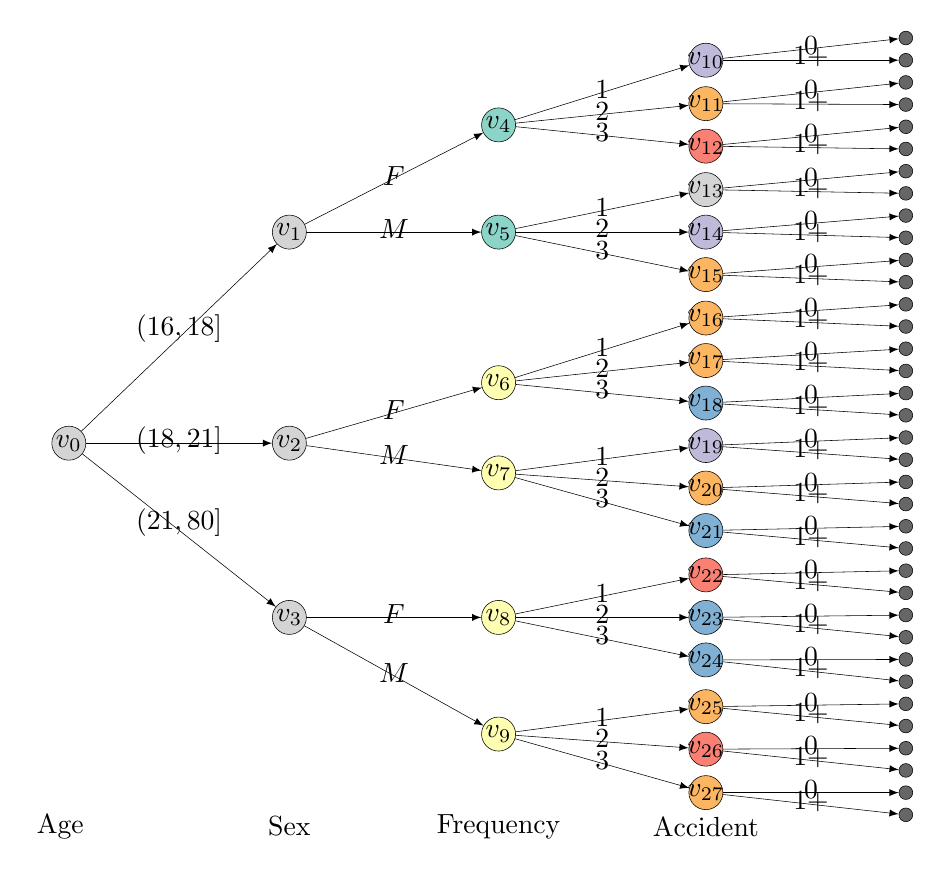
\begin{tikzpicture}[>=latex,line join=bevel, scale = 0.17]
  \pgfsetlinewidth{0.2bp}
%%
\pgfsetcolor{black}
  % Edge: v_{0} -> v_{1}
  \draw [->] (62.109bp,826.49bp) .. controls (141.62bp,902.6bp) and (380.74bp,1131.5bp)  .. (476.79bp,1223.4bp);
  \definecolor{strokecol}{rgb}{0.0,0.0,0.0};
  \pgfsetstrokecolor{strokecol}
  \draw (269.5bp,1044.0bp) node {$(16,18]$};
  % Edge: v_{0} -> v_{2}
  \pgfsetcolor{black}
  \draw [->] (72.256bp,801.5bp) .. controls (156.14bp,801.5bp) and (363.51bp,801.5bp)  .. (466.77bp,801.5bp);
  \definecolor{strokecol}{rgb}{0.0,0.0,0.0};
  \pgfsetstrokecolor{strokecol}
  \draw (269.5bp,808.0bp) node {$(18,21]$};
  % Edge: v_{0} -> v_{3}
  \pgfsetcolor{black}
  \draw [->] (64.51bp,778.97bp) .. controls (145.45bp,715.02bp) and (376.62bp,532.36bp)  .. (474.57bp,454.97bp);
  \definecolor{strokecol}{rgb}{0.0,0.0,0.0};
  \pgfsetstrokecolor{strokecol}
  \draw (269.5bp,634.0bp) node {$(21,80]$};
  % Edge: v_{1} -> v_{4}
  \pgfsetcolor{black}
  \draw [->] (535.22bp,1265.0bp) .. controls (614.17bp,1305.5bp) and (817.24bp,1409.5bp)  .. (913.9bp,1459.1bp);
  \definecolor{strokecol}{rgb}{0.0,0.0,0.0};
  \pgfsetstrokecolor{strokecol}
  \draw (724.5bp,1368.0bp) node {$F$};
  % Edge: v_{1} -> v_{5}
  \pgfsetcolor{black}
  \draw [->] (539.25bp,1248.5bp) .. controls (619.36bp,1248.5bp) and (811.33bp,1248.5bp)  .. (909.87bp,1248.5bp);
  \definecolor{strokecol}{rgb}{0.0,0.0,0.0};
  \pgfsetstrokecolor{strokecol}
  \draw (724.5bp,1255.0bp) node {$M$};
  % Edge: v_{2} -> v_{6}
  \pgfsetcolor{black}
  \draw [->] (537.76bp,811.54bp) .. controls (617.5bp,834.58bp) and (813.47bp,891.21bp)  .. (911.4bp,919.5bp);
  \definecolor{strokecol}{rgb}{0.0,0.0,0.0};
  \pgfsetstrokecolor{strokecol}
  \draw (724.5bp,872.0bp) node {$F$};
  % Edge: v_{2} -> v_{7}
  \pgfsetcolor{black}
  \draw [->] (538.88bp,796.4bp) .. controls (618.83bp,785.03bp) and (811.52bp,757.62bp)  .. (910.1bp,743.61bp);
  \definecolor{strokecol}{rgb}{0.0,0.0,0.0};
  \pgfsetstrokecolor{strokecol}
  \draw (724.5bp,776.0bp) node {$M$};
  % Edge: v_{3} -> v_{8}
  \pgfsetcolor{black}
  \draw [->] (539.25bp,432.5bp) .. controls (619.36bp,432.5bp) and (811.33bp,432.5bp)  .. (909.87bp,432.5bp);
  \definecolor{strokecol}{rgb}{0.0,0.0,0.0};
  \pgfsetstrokecolor{strokecol}
  \draw (724.5bp,439.0bp) node {$F$};
  % Edge: v_{3} -> v_{9}
  \pgfsetcolor{black}
  \draw [->] (534.5bp,414.93bp) .. controls (613.16bp,371.08bp) and (818.11bp,256.81bp)  .. (914.36bp,203.14bp);
  \definecolor{strokecol}{rgb}{0.0,0.0,0.0};
  \pgfsetstrokecolor{strokecol}
  \draw (724.5bp,315.0bp) node {$M$};
  % Edge: v_{4} -> v_{10}
  \pgfsetcolor{black}
  \draw [->] (980.45bp,1486.3bp) .. controls (1059.4bp,1510.9bp) and (1253.2bp,1571.4bp)  .. (1350.4bp,1601.7bp);
  \definecolor{strokecol}{rgb}{0.0,0.0,0.0};
  \pgfsetstrokecolor{strokecol}
  \draw (1165.5bp,1550.0bp) node {$1$};
  % Edge: v_{4} -> v_{11}
  \pgfsetcolor{black}
  \draw [->] (981.93bp,1479.2bp) .. controls (1061.1bp,1487.3bp) and (1250.7bp,1506.7bp)  .. (1348.9bp,1516.8bp);
  \definecolor{strokecol}{rgb}{0.0,0.0,0.0};
  \pgfsetstrokecolor{strokecol}
  \draw (1165.5bp,1504.0bp) node {$2$};
  % Edge: v_{4} -> v_{12}
  \pgfsetcolor{black}
  \draw [->] (981.93bp,1471.8bp) .. controls (1061.1bp,1463.7bp) and (1250.7bp,1444.3bp)  .. (1348.9bp,1434.2bp);
  \definecolor{strokecol}{rgb}{0.0,0.0,0.0};
  \pgfsetstrokecolor{strokecol}
  \draw (1165.5bp,1459.0bp) node {$3$};
  % Edge: v_{5} -> v_{13}
  \pgfsetcolor{black}
  \draw [->] (981.55bp,1255.8bp) .. controls (1060.9bp,1272.1bp) and (1252.2bp,1311.3bp)  .. (1349.7bp,1331.3bp);
  \definecolor{strokecol}{rgb}{0.0,0.0,0.0};
  \pgfsetstrokecolor{strokecol}
  \draw (1165.5bp,1300.0bp) node {$1$};
  % Edge: v_{5} -> v_{14}
  \pgfsetcolor{black}
  \draw [->] (982.3bp,1248.5bp) .. controls (1061.8bp,1248.5bp) and (1251.0bp,1248.5bp)  .. (1349.0bp,1248.5bp);
  \definecolor{strokecol}{rgb}{0.0,0.0,0.0};
  \pgfsetstrokecolor{strokecol}
  \draw (1165.5bp,1255.0bp) node {$2$};
  % Edge: v_{5} -> v_{15}
  \pgfsetcolor{black}
  \draw [->] (981.55bp,1241.2bp) .. controls (1060.9bp,1224.9bp) and (1252.2bp,1185.7bp)  .. (1349.7bp,1165.7bp);
  \definecolor{strokecol}{rgb}{0.0,0.0,0.0};
  \pgfsetstrokecolor{strokecol}
  \draw (1165.5bp,1210.0bp) node {$3$};
  % Edge: v_{6} -> v_{16}
  \pgfsetcolor{black}
  \draw [->] (980.45bp,940.25bp) .. controls (1059.4bp,964.88bp) and (1253.2bp,1025.4bp)  .. (1350.4bp,1055.7bp);
  \definecolor{strokecol}{rgb}{0.0,0.0,0.0};
  \pgfsetstrokecolor{strokecol}
  \draw (1165.5bp,1004.0bp) node {$1$};
  % Edge: v_{6} -> v_{17}
  \pgfsetcolor{black}
  \draw [->] (981.93bp,933.35bp) .. controls (1061.2bp,941.84bp) and (1251.2bp,962.17bp)  .. (1349.2bp,972.67bp);
  \definecolor{strokecol}{rgb}{0.0,0.0,0.0};
  \pgfsetstrokecolor{strokecol}
  \draw (1165.5bp,959.0bp) node {$2$};
  % Edge: v_{6} -> v_{18}
  \pgfsetcolor{black}
  \draw [->] (981.93bp,925.98bp) .. controls (1061.1bp,918.22bp) and (1250.7bp,899.66bp)  .. (1348.9bp,890.04bp);
  \definecolor{strokecol}{rgb}{0.0,0.0,0.0};
  \pgfsetstrokecolor{strokecol}
  \draw (1165.5bp,914.0bp) node {$3$};
  % Edge: v_{7} -> v_{19}
  \pgfsetcolor{black}
  \draw [->] (981.93bp,743.25bp) .. controls (1061.3bp,753.73bp) and (1251.5bp,778.87bp)  .. (1349.2bp,791.77bp);
  \definecolor{strokecol}{rgb}{0.0,0.0,0.0};
  \pgfsetstrokecolor{strokecol}
  \draw (1165.5bp,774.0bp) node {$1$};
  % Edge: v_{7} -> v_{20}
  \pgfsetcolor{black}
  \draw [->] (981.93bp,735.88bp) .. controls (1061.1bp,730.11bp) and (1250.7bp,716.29bp)  .. (1348.9bp,709.13bp);
  \definecolor{strokecol}{rgb}{0.0,0.0,0.0};
  \pgfsetstrokecolor{strokecol}
  \draw (1165.5bp,729.0bp) node {$2$};
  % Edge: v_{7} -> v_{21}
  \pgfsetcolor{black}
  \draw [->] (980.81bp,728.82bp) .. controls (1059.9bp,706.85bp) and (1253.0bp,653.19bp)  .. (1350.2bp,626.18bp);
  \definecolor{strokecol}{rgb}{0.0,0.0,0.0};
  \pgfsetstrokecolor{strokecol}
  \draw (1165.5bp,684.0bp) node {$3$};
  % Edge: v_{8} -> v_{22}
  \pgfsetcolor{black}
  \draw [->] (981.55bp,439.79bp) .. controls (1060.9bp,456.05bp) and (1252.2bp,495.28bp)  .. (1349.7bp,515.27bp);
  \definecolor{strokecol}{rgb}{0.0,0.0,0.0};
  \pgfsetstrokecolor{strokecol}
  \draw (1165.5bp,484.0bp) node {$1$};
  % Edge: v_{8} -> v_{23}
  \pgfsetcolor{black}
  \draw [->] (982.3bp,432.5bp) .. controls (1061.8bp,432.5bp) and (1251.0bp,432.5bp)  .. (1349.0bp,432.5bp);
  \definecolor{strokecol}{rgb}{0.0,0.0,0.0};
  \pgfsetstrokecolor{strokecol}
  \draw (1165.5bp,439.0bp) node {$2$};
  % Edge: v_{8} -> v_{24}
  \pgfsetcolor{black}
  \draw [->] (981.55bp,425.21bp) .. controls (1060.9bp,408.95bp) and (1252.2bp,369.72bp)  .. (1349.7bp,349.73bp);
  \definecolor{strokecol}{rgb}{0.0,0.0,0.0};
  \pgfsetstrokecolor{strokecol}
  \draw (1165.5bp,394.0bp) node {$3$};
  % Edge: v_{9} -> v_{25}
  \pgfsetcolor{black}
  \draw [->] (981.93bp,190.25bp) .. controls (1061.3bp,200.73bp) and (1251.5bp,225.87bp)  .. (1349.2bp,238.77bp);
  \definecolor{strokecol}{rgb}{0.0,0.0,0.0};
  \pgfsetstrokecolor{strokecol}
  \draw (1165.5bp,221.0bp) node {$1$};
  % Edge: v_{9} -> v_{26}
  \pgfsetcolor{black}
  \draw [->] (981.93bp,182.88bp) .. controls (1061.1bp,177.11bp) and (1250.7bp,163.29bp)  .. (1348.9bp,156.13bp);
  \definecolor{strokecol}{rgb}{0.0,0.0,0.0};
  \pgfsetstrokecolor{strokecol}
  \draw (1165.5bp,176.0bp) node {$2$};
  % Edge: v_{9} -> v_{27}
  \pgfsetcolor{black}
  \draw [->] (980.81bp,175.67bp) .. controls (1059.9bp,153.33bp) and (1253.0bp,98.787bp)  .. (1350.2bp,71.335bp);
  \definecolor{strokecol}{rgb}{0.0,0.0,0.0};
  \pgfsetstrokecolor{strokecol}
  \draw (1165.5bp,130.0bp) node {$3$};
  % Edge: v_{10} -> v_{28}
  \pgfsetcolor{black}
  \draw [->] (1421.1bp,1616.5bp) .. controls (1505.0bp,1625.8bp) and (1711.5bp,1648.7bp)  .. (1793.7bp,1657.9bp);
  \definecolor{strokecol}{rgb}{0.0,0.0,0.0};
  \pgfsetstrokecolor{strokecol}
  \draw (1607.5bp,1643.0bp) node {$0$};
  % Edge: v_{10} -> v_{29}
  \pgfsetcolor{black}
  \draw [->] (1421.1bp,1612.5bp) .. controls (1505.0bp,1612.5bp) and (1711.5bp,1612.5bp)  .. (1793.7bp,1612.5bp);
  \definecolor{strokecol}{rgb}{0.0,0.0,0.0};
  \pgfsetstrokecolor{strokecol}
  \draw (1607.5bp,1619.0bp) node {$1+$};
  % Edge: v_{11} -> v_{30}
  \pgfsetcolor{black}
  \draw [->] (1421.1bp,1524.3bp) .. controls (1505.0bp,1533.3bp) and (1711.5bp,1555.2bp)  .. (1793.7bp,1563.9bp);
  \definecolor{strokecol}{rgb}{0.0,0.0,0.0};
  \pgfsetstrokecolor{strokecol}
  \draw (1607.5bp,1550.0bp) node {$0$};
  % Edge: v_{11} -> v_{31}
  \pgfsetcolor{black}
  \draw [->] (1421.1bp,1520.3bp) .. controls (1505.0bp,1519.9bp) and (1711.5bp,1519.0bp)  .. (1793.7bp,1518.6bp);
  \definecolor{strokecol}{rgb}{0.0,0.0,0.0};
  \pgfsetstrokecolor{strokecol}
  \draw (1607.5bp,1525.0bp) node {$1+$};
  % Edge: v_{12} -> v_{32}
  \pgfsetcolor{black}
  \draw [->] (1421.1bp,1434.0bp) .. controls (1505.0bp,1442.1bp) and (1711.5bp,1462.1bp)  .. (1793.7bp,1470.1bp);
  \definecolor{strokecol}{rgb}{0.0,0.0,0.0};
  \pgfsetstrokecolor{strokecol}
  \draw (1607.5bp,1458.0bp) node {$0$};
  % Edge: v_{12} -> v_{33}
  \pgfsetcolor{black}
  \draw [->] (1421.1bp,1430.0bp) .. controls (1505.0bp,1428.8bp) and (1711.5bp,1425.9bp)  .. (1793.7bp,1424.7bp);
  \definecolor{strokecol}{rgb}{0.0,0.0,0.0};
  \pgfsetstrokecolor{strokecol}
  \draw (1607.5bp,1433.0bp) node {$1+$};
  % Edge: v_{13} -> v_{34}
  \pgfsetcolor{black}
  \draw [->] (1421.1bp,1341.8bp) .. controls (1505.0bp,1349.6bp) and (1711.5bp,1368.6bp)  .. (1793.7bp,1376.1bp);
  \definecolor{strokecol}{rgb}{0.0,0.0,0.0};
  \pgfsetstrokecolor{strokecol}
  \draw (1607.5bp,1365.0bp) node {$0$};
  % Edge: v_{13} -> v_{35}
  \pgfsetcolor{black}
  \draw [->] (1421.1bp,1337.8bp) .. controls (1505.0bp,1336.2bp) and (1711.5bp,1332.3bp)  .. (1793.7bp,1330.8bp);
  \definecolor{strokecol}{rgb}{0.0,0.0,0.0};
  \pgfsetstrokecolor{strokecol}
  \draw (1607.5bp,1340.0bp) node {$1+$};
  % Edge: v_{14} -> v_{36}
  \pgfsetcolor{black}
  \draw [->] (1421.1bp,1251.5bp) .. controls (1505.0bp,1258.4bp) and (1711.5bp,1275.5bp)  .. (1793.7bp,1282.3bp);
  \definecolor{strokecol}{rgb}{0.0,0.0,0.0};
  \pgfsetstrokecolor{strokecol}
  \draw (1607.5bp,1273.0bp) node {$0$};
  % Edge: v_{14} -> v_{37}
  \pgfsetcolor{black}
  \draw [->] (1421.1bp,1247.5bp) .. controls (1505.0bp,1245.1bp) and (1711.5bp,1239.2bp)  .. (1793.7bp,1236.9bp);
  \definecolor{strokecol}{rgb}{0.0,0.0,0.0};
  \pgfsetstrokecolor{strokecol}
  \draw (1607.5bp,1248.0bp) node {$1+$};
  % Edge: v_{15} -> v_{38}
  \pgfsetcolor{black}
  \draw [->] (1421.1bp,1161.1bp) .. controls (1505.0bp,1167.3bp) and (1711.5bp,1182.4bp)  .. (1793.7bp,1188.4bp);
  \definecolor{strokecol}{rgb}{0.0,0.0,0.0};
  \pgfsetstrokecolor{strokecol}
  \draw (1607.5bp,1181.0bp) node {$0$};
  % Edge: v_{15} -> v_{39}
  \pgfsetcolor{black}
  \draw [->] (1421.1bp,1157.1bp) .. controls (1505.0bp,1154.0bp) and (1711.5bp,1146.2bp)  .. (1793.7bp,1143.1bp);
  \definecolor{strokecol}{rgb}{0.0,0.0,0.0};
  \pgfsetstrokecolor{strokecol}
  \draw (1607.5bp,1156.0bp) node {$1+$};
  % Edge: v_{16} -> v_{40}
  \pgfsetcolor{black}
  \draw [->] (1421.1bp,1069.0bp) .. controls (1505.0bp,1074.7bp) and (1711.5bp,1088.9bp)  .. (1793.7bp,1094.5bp);
  \definecolor{strokecol}{rgb}{0.0,0.0,0.0};
  \pgfsetstrokecolor{strokecol}
  \draw (1607.5bp,1088.0bp) node {$0$};
  % Edge: v_{16} -> v_{41}
  \pgfsetcolor{black}
  \draw [->] (1421.1bp,1065.0bp) .. controls (1505.0bp,1061.4bp) and (1711.5bp,1052.6bp)  .. (1793.7bp,1049.1bp);
  \definecolor{strokecol}{rgb}{0.0,0.0,0.0};
  \pgfsetstrokecolor{strokecol}
  \draw (1607.5bp,1063.0bp) node {$1+$};
  % Edge: v_{17} -> v_{42}
  \pgfsetcolor{black}
  \draw [->] (1421.1bp,978.63bp) .. controls (1505.0bp,983.59bp) and (1711.5bp,995.78bp)  .. (1793.7bp,1000.6bp);
  \definecolor{strokecol}{rgb}{0.0,0.0,0.0};
  \pgfsetstrokecolor{strokecol}
  \draw (1607.5bp,996.0bp) node {$0$};
  % Edge: v_{17} -> v_{43}
  \pgfsetcolor{black}
  \draw [->] (1421.1bp,974.62bp) .. controls (1505.0bp,970.26bp) and (1711.5bp,959.54bp)  .. (1793.7bp,955.27bp);
  \definecolor{strokecol}{rgb}{0.0,0.0,0.0};
  \pgfsetstrokecolor{strokecol}
  \draw (1607.5bp,971.0bp) node {$1+$};
  % Edge: v_{18} -> v_{44}
  \pgfsetcolor{black}
  \draw [->] (1421.1bp,888.29bp) .. controls (1505.0bp,892.45bp) and (1711.5bp,902.69bp)  .. (1793.7bp,906.77bp);
  \definecolor{strokecol}{rgb}{0.0,0.0,0.0};
  \pgfsetstrokecolor{strokecol}
  \draw (1607.5bp,904.0bp) node {$0$};
  % Edge: v_{18} -> v_{45}
  \pgfsetcolor{black}
  \draw [->] (1421.1bp,884.28bp) .. controls (1505.0bp,879.13bp) and (1711.5bp,866.45bp)  .. (1793.7bp,861.41bp);
  \definecolor{strokecol}{rgb}{0.0,0.0,0.0};
  \pgfsetstrokecolor{strokecol}
  \draw (1607.5bp,879.0bp) node {$1+$};
  % Edge: v_{19} -> v_{46}
  \pgfsetcolor{black}
  \draw [->] (1421.1bp,797.95bp) .. controls (1505.0bp,801.32bp) and (1711.5bp,809.61bp)  .. (1793.7bp,812.91bp);
  \definecolor{strokecol}{rgb}{0.0,0.0,0.0};
  \pgfsetstrokecolor{strokecol}
  \draw (1607.5bp,812.0bp) node {$0$};
  % Edge: v_{19} -> v_{47}
  \pgfsetcolor{black}
  \draw [->] (1421.1bp,793.94bp) .. controls (1505.0bp,788.0bp) and (1711.5bp,773.37bp)  .. (1793.7bp,767.55bp);
  \definecolor{strokecol}{rgb}{0.0,0.0,0.0};
  \pgfsetstrokecolor{strokecol}
  \draw (1607.5bp,787.0bp) node {$1+$};
  % Edge: v_{20} -> v_{48}
  \pgfsetcolor{black}
  \draw [->] (1421.1bp,707.61bp) .. controls (1505.0bp,710.18bp) and (1711.5bp,716.52bp)  .. (1793.7bp,719.05bp);
  \definecolor{strokecol}{rgb}{0.0,0.0,0.0};
  \pgfsetstrokecolor{strokecol}
  \draw (1607.5bp,719.0bp) node {$0$};
  % Edge: v_{20} -> v_{49}
  \pgfsetcolor{black}
  \draw [->] (1421.1bp,703.6bp) .. controls (1505.0bp,696.86bp) and (1711.5bp,680.28bp)  .. (1793.7bp,673.69bp);
  \definecolor{strokecol}{rgb}{0.0,0.0,0.0};
  \pgfsetstrokecolor{strokecol}
  \draw (1607.5bp,694.0bp) node {$1+$};
  % Edge: v_{21} -> v_{50}
  \pgfsetcolor{black}
  \draw [->] (1421.1bp,617.27bp) .. controls (1505.0bp,619.05bp) and (1711.5bp,623.44bp)  .. (1793.7bp,625.19bp);
  \definecolor{strokecol}{rgb}{0.0,0.0,0.0};
  \pgfsetstrokecolor{strokecol}
  \draw (1607.5bp,627.0bp) node {$0$};
  % Edge: v_{21} -> v_{51}
  \pgfsetcolor{black}
  \draw [->] (1421.1bp,613.26bp) .. controls (1505.0bp,605.73bp) and (1711.5bp,587.2bp)  .. (1793.7bp,579.83bp);
  \definecolor{strokecol}{rgb}{0.0,0.0,0.0};
  \pgfsetstrokecolor{strokecol}
  \draw (1607.5bp,602.0bp) node {$1+$};
  % Edge: v_{22} -> v_{52}
  \pgfsetcolor{black}
  \draw [->] (1421.1bp,523.27bp) .. controls (1505.0bp,525.05bp) and (1711.5bp,529.44bp)  .. (1793.7bp,531.19bp);
  \definecolor{strokecol}{rgb}{0.0,0.0,0.0};
  \pgfsetstrokecolor{strokecol}
  \draw (1607.5bp,533.0bp) node {$0$};
  % Edge: v_{22} -> v_{53}
  \pgfsetcolor{black}
  \draw [->] (1421.1bp,519.26bp) .. controls (1505.0bp,511.73bp) and (1711.5bp,493.2bp)  .. (1793.7bp,485.83bp);
  \definecolor{strokecol}{rgb}{0.0,0.0,0.0};
  \pgfsetstrokecolor{strokecol}
  \draw (1607.5bp,508.0bp) node {$1+$};
  % Edge: v_{23} -> v_{54}
  \pgfsetcolor{black}
  \draw [->] (1421.1bp,432.93bp) .. controls (1505.0bp,433.92bp) and (1711.5bp,436.36bp)  .. (1793.7bp,437.33bp);
  \definecolor{strokecol}{rgb}{0.0,0.0,0.0};
  \pgfsetstrokecolor{strokecol}
  \draw (1607.5bp,441.0bp) node {$0$};
  % Edge: v_{23} -> v_{55}
  \pgfsetcolor{black}
  \draw [->] (1421.1bp,428.92bp) .. controls (1505.0bp,420.6bp) and (1711.5bp,400.12bp)  .. (1793.7bp,391.97bp);
  \definecolor{strokecol}{rgb}{0.0,0.0,0.0};
  \pgfsetstrokecolor{strokecol}
  \draw (1607.5bp,416.0bp) node {$1+$};
  % Edge: v_{24} -> v_{56}
  \pgfsetcolor{black}
  \draw [->] (1421.1bp,342.59bp) .. controls (1505.0bp,342.78bp) and (1711.5bp,343.27bp)  .. (1793.7bp,343.47bp);
  \definecolor{strokecol}{rgb}{0.0,0.0,0.0};
  \pgfsetstrokecolor{strokecol}
  \draw (1607.5bp,349.0bp) node {$0$};
  % Edge: v_{24} -> v_{57}
  \pgfsetcolor{black}
  \draw [->] (1421.1bp,338.58bp) .. controls (1505.0bp,329.46bp) and (1711.5bp,307.03bp)  .. (1793.7bp,298.11bp);
  \definecolor{strokecol}{rgb}{0.0,0.0,0.0};
  \pgfsetstrokecolor{strokecol}
  \draw (1607.5bp,324.0bp) node {$1+$};
  % Edge: v_{25} -> v_{58}
  \pgfsetcolor{black}
  \draw [->] (1421.1bp,244.01bp) .. controls (1505.0bp,245.2bp) and (1711.5bp,248.13bp)  .. (1793.7bp,249.29bp);
  \definecolor{strokecol}{rgb}{0.0,0.0,0.0};
  \pgfsetstrokecolor{strokecol}
  \draw (1607.5bp,253.0bp) node {$0$};
  % Edge: v_{25} -> v_{59}
  \pgfsetcolor{black}
  \draw [->] (1421.1bp,240.0bp) .. controls (1505.0bp,231.88bp) and (1711.5bp,211.89bp)  .. (1793.7bp,203.93bp);
  \definecolor{strokecol}{rgb}{0.0,0.0,0.0};
  \pgfsetstrokecolor{strokecol}
  \draw (1607.5bp,228.0bp) node {$1+$};
  % Edge: v_{26} -> v_{60}
  \pgfsetcolor{black}
  \draw [->] (1421.1bp,153.67bp) .. controls (1505.0bp,154.07bp) and (1711.5bp,155.04bp)  .. (1793.7bp,155.43bp);
  \definecolor{strokecol}{rgb}{0.0,0.0,0.0};
  \pgfsetstrokecolor{strokecol}
  \draw (1607.5bp,161.0bp) node {$0$};
  % Edge: v_{26} -> v_{61}
  \pgfsetcolor{black}
  \draw [->] (1421.1bp,149.66bp) .. controls (1505.0bp,140.75bp) and (1711.5bp,118.8bp)  .. (1793.7bp,110.07bp);
  \definecolor{strokecol}{rgb}{0.0,0.0,0.0};
  \pgfsetstrokecolor{strokecol}
  \draw (1607.5bp,136.0bp) node {$1+$};
  % Edge: v_{27} -> v_{62}
  \pgfsetcolor{black}
  \draw [->] (1421.1bp,61.5bp) .. controls (1505.0bp,61.5bp) and (1711.5bp,61.5bp)  .. (1793.7bp,61.5bp);
  \definecolor{strokecol}{rgb}{0.0,0.0,0.0};
  \pgfsetstrokecolor{strokecol}
  \draw (1607.5bp,68.0bp) node {$0$};
  % Edge: v_{27} -> v_{63}
  \pgfsetcolor{black}
  \draw [->] (1421.1bp,57.493bp) .. controls (1505.0bp,48.179bp) and (1711.5bp,25.26bp)  .. (1793.7bp,16.141bp);
  \definecolor{strokecol}{rgb}{0.0,0.0,0.0};
  \pgfsetstrokecolor{strokecol}
  \draw (1607.5bp,43.0bp) node {$1+$};
  % Node: v_{0}
\begin{scope}
  \definecolor{strokecol}{rgb}{0.0,0.0,0.0};
  \pgfsetstrokecolor{strokecol}
  \definecolor{fillcol}{rgb}{0.83,0.83,0.83};
  \pgfsetfillcolor{fillcol}
  \filldraw [opacity=1] (36.0bp,801.5bp) ellipse (36.0bp and 36.0bp);
  \draw (36.0bp,801.5bp) node {$v_{0}$};
\end{scope}
  % Node: v_{1}
\begin{scope}
  \definecolor{strokecol}{rgb}{0.0,0.0,0.0};
  \pgfsetstrokecolor{strokecol}
  \definecolor{fillcol}{rgb}{0.83,0.83,0.83};
  \pgfsetfillcolor{fillcol}
  \filldraw [opacity=1] (503.0bp,1248.5bp) ellipse (36.0bp and 36.0bp);
  \draw (503.0bp,1248.5bp) node {$v_{1}$};
\end{scope}
  % Node: v_{2}
\begin{scope}
  \definecolor{strokecol}{rgb}{0.0,0.0,0.0};
  \pgfsetstrokecolor{strokecol}
  \definecolor{fillcol}{rgb}{0.83,0.83,0.83};
  \pgfsetfillcolor{fillcol}
  \filldraw [opacity=1] (503.0bp,801.5bp) ellipse (36.0bp and 36.0bp);
  \draw (503.0bp,801.5bp) node {$v_{2}$};
\end{scope}
  % Node: v_{3}
\begin{scope}
  \definecolor{strokecol}{rgb}{0.0,0.0,0.0};
  \pgfsetstrokecolor{strokecol}
  \definecolor{fillcol}{rgb}{0.83,0.83,0.83};
  \pgfsetfillcolor{fillcol}
  \filldraw [opacity=1] (503.0bp,432.5bp) ellipse (36.0bp and 36.0bp);
  \draw (503.0bp,432.5bp) node {$v_{3}$};
\end{scope}
  % Node: v_{4}
\begin{scope}
  \definecolor{strokecol}{rgb}{0.0,0.0,0.0};
  \pgfsetstrokecolor{strokecol}
  \definecolor{fillcol}{rgb}{0.55,0.83,0.78};
  \pgfsetfillcolor{fillcol}
  \filldraw [opacity=1] (946.0bp,1475.5bp) ellipse (36.0bp and 36.0bp);
  \draw (946.0bp,1475.5bp) node {$v_{4}$};
\end{scope}
  % Node: v_{5}
\begin{scope}
  \definecolor{strokecol}{rgb}{0.0,0.0,0.0};
  \pgfsetstrokecolor{strokecol}
  \definecolor{fillcol}{rgb}{0.55,0.83,0.78};
  \pgfsetfillcolor{fillcol}
  \filldraw [opacity=1] (946.0bp,1248.5bp) ellipse (36.0bp and 36.0bp);
  \draw (946.0bp,1248.5bp) node {$v_{5}$};
\end{scope}
  % Node: v_{6}
\begin{scope}
  \definecolor{strokecol}{rgb}{0.0,0.0,0.0};
  \pgfsetstrokecolor{strokecol}
  \definecolor{fillcol}{rgb}{1.0,1.0,0.7};
  \pgfsetfillcolor{fillcol}
  \filldraw [opacity=1] (946.0bp,929.5bp) ellipse (36.0bp and 36.0bp);
  \draw (946.0bp,929.5bp) node {$v_{6}$};
\end{scope}
  % Node: v_{7}
\begin{scope}
  \definecolor{strokecol}{rgb}{0.0,0.0,0.0};
  \pgfsetstrokecolor{strokecol}
  \definecolor{fillcol}{rgb}{1.0,1.0,0.7};
  \pgfsetfillcolor{fillcol}
  \filldraw [opacity=1] (946.0bp,738.5bp) ellipse (36.0bp and 36.0bp);
  \draw (946.0bp,738.5bp) node {$v_{7}$};
\end{scope}
  % Node: v_{8}
\begin{scope}
  \definecolor{strokecol}{rgb}{0.0,0.0,0.0};
  \pgfsetstrokecolor{strokecol}
  \definecolor{fillcol}{rgb}{1.0,1.0,0.7};
  \pgfsetfillcolor{fillcol}
  \filldraw [opacity=1] (946.0bp,432.5bp) ellipse (36.0bp and 36.0bp);
  \draw (946.0bp,432.5bp) node {$v_{8}$};
\end{scope}
  % Node: v_{9}
\begin{scope}
  \definecolor{strokecol}{rgb}{0.0,0.0,0.0};
  \pgfsetstrokecolor{strokecol}
  \definecolor{fillcol}{rgb}{1.0,1.0,0.7};
  \pgfsetfillcolor{fillcol}
  \filldraw [opacity=1] (946.0bp,185.5bp) ellipse (36.0bp and 36.0bp);
  \draw (946.0bp,185.5bp) node {$v_{9}$};
\end{scope}
  % Node: v_{10}
\begin{scope}
  \definecolor{strokecol}{rgb}{0.0,0.0,0.0};
  \pgfsetstrokecolor{strokecol}
  \definecolor{fillcol}{rgb}{0.75,0.73,0.85};
  \pgfsetfillcolor{fillcol}
  \filldraw [opacity=1] (1385.0bp,1612.5bp) ellipse (36.0bp and 36.0bp);
  \draw (1385.0bp,1612.5bp) node {$v_{10}$};
\end{scope}
  % Node: v_{11}
\begin{scope}
  \definecolor{strokecol}{rgb}{0.0,0.0,0.0};
  \pgfsetstrokecolor{strokecol}
  \definecolor{fillcol}{rgb}{0.99,0.71,0.38};
  \pgfsetfillcolor{fillcol}
  \filldraw [opacity=1] (1385.0bp,1520.5bp) ellipse (36.0bp and 36.0bp);
  \draw (1385.0bp,1520.5bp) node {$v_{11}$};
\end{scope}
  % Node: v_{12}
\begin{scope}
  \definecolor{strokecol}{rgb}{0.0,0.0,0.0};
  \pgfsetstrokecolor{strokecol}
  \definecolor{fillcol}{rgb}{0.98,0.5,0.45};
  \pgfsetfillcolor{fillcol}
  \filldraw [opacity=1] (1385.0bp,1430.5bp) ellipse (36.0bp and 36.0bp);
  \draw (1385.0bp,1430.5bp) node {$v_{12}$};
\end{scope}
  % Node: v_{13}
\begin{scope}
  \definecolor{strokecol}{rgb}{0.0,0.0,0.0};
  \pgfsetstrokecolor{strokecol}
  \definecolor{fillcol}{rgb}{0.83,0.83,0.83};
  \pgfsetfillcolor{fillcol}
  \filldraw [opacity=1] (1385.0bp,1338.5bp) ellipse (36.0bp and 36.0bp);
  \draw (1385.0bp,1338.5bp) node {$v_{13}$};
\end{scope}
  % Node: v_{14}
\begin{scope}
  \definecolor{strokecol}{rgb}{0.0,0.0,0.0};
  \pgfsetstrokecolor{strokecol}
  \definecolor{fillcol}{rgb}{0.75,0.73,0.85};
  \pgfsetfillcolor{fillcol}
  \filldraw [opacity=1] (1385.0bp,1248.5bp) ellipse (36.0bp and 36.0bp);
  \draw (1385.0bp,1248.5bp) node {$v_{14}$};
\end{scope}
  % Node: v_{15}
\begin{scope}
  \definecolor{strokecol}{rgb}{0.0,0.0,0.0};
  \pgfsetstrokecolor{strokecol}
  \definecolor{fillcol}{rgb}{0.99,0.71,0.38};
  \pgfsetfillcolor{fillcol}
  \filldraw [opacity=1] (1385.0bp,1158.5bp) ellipse (36.0bp and 36.0bp);
  \draw (1385.0bp,1158.5bp) node {$v_{15}$};
\end{scope}
  % Node: v_{16}
\begin{scope}
  \definecolor{strokecol}{rgb}{0.0,0.0,0.0};
  \pgfsetstrokecolor{strokecol}
  \definecolor{fillcol}{rgb}{0.99,0.71,0.38};
  \pgfsetfillcolor{fillcol}
  \filldraw [opacity=1] (1385.0bp,1066.5bp) ellipse (36.0bp and 36.0bp);
  \draw (1385.0bp,1066.5bp) node {$v_{16}$};
\end{scope}
  % Node: v_{17}
\begin{scope}
  \definecolor{strokecol}{rgb}{0.0,0.0,0.0};
  \pgfsetstrokecolor{strokecol}
  \definecolor{fillcol}{rgb}{0.99,0.71,0.38};
  \pgfsetfillcolor{fillcol}
  \filldraw [opacity=1] (1385.0bp,976.5bp) ellipse (36.0bp and 36.0bp);
  \draw (1385.0bp,976.5bp) node {$v_{17}$};
\end{scope}
  % Node: v_{18}
\begin{scope}
  \definecolor{strokecol}{rgb}{0.0,0.0,0.0};
  \pgfsetstrokecolor{strokecol}
  \definecolor{fillcol}{rgb}{0.5,0.69,0.83};
  \pgfsetfillcolor{fillcol}
  \filldraw [opacity=1] (1385.0bp,886.5bp) ellipse (36.0bp and 36.0bp);
  \draw (1385.0bp,886.5bp) node {$v_{18}$};
\end{scope}
  % Node: v_{19}
\begin{scope}
  \definecolor{strokecol}{rgb}{0.0,0.0,0.0};
  \pgfsetstrokecolor{strokecol}
  \definecolor{fillcol}{rgb}{0.75,0.73,0.85};
  \pgfsetfillcolor{fillcol}
  \filldraw [opacity=1] (1385.0bp,796.5bp) ellipse (36.0bp and 36.0bp);
  \draw (1385.0bp,796.5bp) node {$v_{19}$};
\end{scope}
  % Node: v_{20}
\begin{scope}
  \definecolor{strokecol}{rgb}{0.0,0.0,0.0};
  \pgfsetstrokecolor{strokecol}
  \definecolor{fillcol}{rgb}{0.99,0.71,0.38};
  \pgfsetfillcolor{fillcol}
  \filldraw [opacity=1] (1385.0bp,706.5bp) ellipse (36.0bp and 36.0bp);
  \draw (1385.0bp,706.5bp) node {$v_{20}$};
\end{scope}
  % Node: v_{21}
\begin{scope}
  \definecolor{strokecol}{rgb}{0.0,0.0,0.0};
  \pgfsetstrokecolor{strokecol}
  \definecolor{fillcol}{rgb}{0.5,0.69,0.83};
  \pgfsetfillcolor{fillcol}
  \filldraw [opacity=1] (1385.0bp,616.5bp) ellipse (36.0bp and 36.0bp);
  \draw (1385.0bp,616.5bp) node {$v_{21}$};
\end{scope}
  % Node: v_{22}
\begin{scope}
  \definecolor{strokecol}{rgb}{0.0,0.0,0.0};
  \pgfsetstrokecolor{strokecol}
  \definecolor{fillcol}{rgb}{0.98,0.5,0.45};
  \pgfsetfillcolor{fillcol}
  \filldraw [opacity=1] (1385.0bp,522.5bp) ellipse (36.0bp and 36.0bp);
  \draw (1385.0bp,522.5bp) node {$v_{22}$};
\end{scope}
  % Node: v_{23}
\begin{scope}
  \definecolor{strokecol}{rgb}{0.0,0.0,0.0};
  \pgfsetstrokecolor{strokecol}
  \definecolor{fillcol}{rgb}{0.5,0.69,0.83};
  \pgfsetfillcolor{fillcol}
  \filldraw [opacity=1] (1385.0bp,432.5bp) ellipse (36.0bp and 36.0bp);
  \draw (1385.0bp,432.5bp) node {$v_{23}$};
\end{scope}
  % Node: v_{24}
\begin{scope}
  \definecolor{strokecol}{rgb}{0.0,0.0,0.0};
  \pgfsetstrokecolor{strokecol}
  \definecolor{fillcol}{rgb}{0.5,0.69,0.83};
  \pgfsetfillcolor{fillcol}
  \filldraw [opacity=1] (1385.0bp,342.5bp) ellipse (36.0bp and 36.0bp);
  \draw (1385.0bp,342.5bp) node {$v_{24}$};
\end{scope}
  % Node: v_{25}
\begin{scope}
  \definecolor{strokecol}{rgb}{0.0,0.0,0.0};
  \pgfsetstrokecolor{strokecol}
  \definecolor{fillcol}{rgb}{0.99,0.71,0.38};
  \pgfsetfillcolor{fillcol}
  \filldraw [opacity=1] (1385.0bp,243.5bp) ellipse (36.0bp and 36.0bp);
  \draw (1385.0bp,243.5bp) node {$v_{25}$};
\end{scope}
  % Node: v_{26}
\begin{scope}
  \definecolor{strokecol}{rgb}{0.0,0.0,0.0};
  \pgfsetstrokecolor{strokecol}
  \definecolor{fillcol}{rgb}{0.98,0.5,0.45};
  \pgfsetfillcolor{fillcol}
  \filldraw [opacity=1] (1385.0bp,153.5bp) ellipse (36.0bp and 36.0bp);
  \draw (1385.0bp,153.5bp) node {$v_{26}$};
\end{scope}
  % Node: v_{27}
\begin{scope}
  \definecolor{strokecol}{rgb}{0.0,0.0,0.0};
  \pgfsetstrokecolor{strokecol}
  \definecolor{fillcol}{rgb}{0.99,0.71,0.38};
  \pgfsetfillcolor{fillcol}
  \filldraw [opacity=1] (1385.0bp,61.5bp) ellipse (36.0bp and 36.0bp);
  \draw (1385.0bp,61.5bp) node {$v_{27}$};
\end{scope}
  % Node: v_{28}
\begin{scope}
  \definecolor{strokecol}{rgb}{0.0,0.0,0.0};
  \pgfsetstrokecolor{strokecol}
  \definecolor{fillcol}{rgb}{0.4,0.4,0.4};
  \pgfsetfillcolor{fillcol}
  \filldraw [opacity=1] (1808.5bp,1659.5bp) ellipse (14.5bp and 14.5bp);
\end{scope}
  % Node: v_{29}
\begin{scope}
  \definecolor{strokecol}{rgb}{0.0,0.0,0.0};
  \pgfsetstrokecolor{strokecol}
  \definecolor{fillcol}{rgb}{0.4,0.4,0.4};
  \pgfsetfillcolor{fillcol}
  \filldraw [opacity=1] (1808.5bp,1612.5bp) ellipse (14.5bp and 14.5bp);
\end{scope}
  % Node: v_{30}
\begin{scope}
  \definecolor{strokecol}{rgb}{0.0,0.0,0.0};
  \pgfsetstrokecolor{strokecol}
  \definecolor{fillcol}{rgb}{0.4,0.4,0.4};
  \pgfsetfillcolor{fillcol}
  \filldraw [opacity=1] (1808.5bp,1565.5bp) ellipse (14.5bp and 14.5bp);
\end{scope}
  % Node: v_{31}
\begin{scope}
  \definecolor{strokecol}{rgb}{0.0,0.0,0.0};
  \pgfsetstrokecolor{strokecol}
  \definecolor{fillcol}{rgb}{0.4,0.4,0.4};
  \pgfsetfillcolor{fillcol}
  \filldraw [opacity=1] (1808.5bp,1518.5bp) ellipse (14.5bp and 14.5bp);
\end{scope}
  % Node: v_{32}
\begin{scope}
  \definecolor{strokecol}{rgb}{0.0,0.0,0.0};
  \pgfsetstrokecolor{strokecol}
  \definecolor{fillcol}{rgb}{0.4,0.4,0.4};
  \pgfsetfillcolor{fillcol}
  \filldraw [opacity=1] (1808.5bp,1471.5bp) ellipse (14.5bp and 14.5bp);
\end{scope}
  % Node: v_{33}
\begin{scope}
  \definecolor{strokecol}{rgb}{0.0,0.0,0.0};
  \pgfsetstrokecolor{strokecol}
  \definecolor{fillcol}{rgb}{0.4,0.4,0.4};
  \pgfsetfillcolor{fillcol}
  \filldraw [opacity=1] (1808.5bp,1424.5bp) ellipse (14.5bp and 14.5bp);
\end{scope}
  % Node: v_{34}
\begin{scope}
  \definecolor{strokecol}{rgb}{0.0,0.0,0.0};
  \pgfsetstrokecolor{strokecol}
  \definecolor{fillcol}{rgb}{0.4,0.4,0.4};
  \pgfsetfillcolor{fillcol}
  \filldraw [opacity=1] (1808.5bp,1377.5bp) ellipse (14.5bp and 14.5bp);
\end{scope}
  % Node: v_{35}
\begin{scope}
  \definecolor{strokecol}{rgb}{0.0,0.0,0.0};
  \pgfsetstrokecolor{strokecol}
  \definecolor{fillcol}{rgb}{0.4,0.4,0.4};
  \pgfsetfillcolor{fillcol}
  \filldraw [opacity=1] (1808.5bp,1330.5bp) ellipse (14.5bp and 14.5bp);
\end{scope}
  % Node: v_{36}
\begin{scope}
  \definecolor{strokecol}{rgb}{0.0,0.0,0.0};
  \pgfsetstrokecolor{strokecol}
  \definecolor{fillcol}{rgb}{0.4,0.4,0.4};
  \pgfsetfillcolor{fillcol}
  \filldraw [opacity=1] (1808.5bp,1283.5bp) ellipse (14.5bp and 14.5bp);
\end{scope}
  % Node: v_{37}
\begin{scope}
  \definecolor{strokecol}{rgb}{0.0,0.0,0.0};
  \pgfsetstrokecolor{strokecol}
  \definecolor{fillcol}{rgb}{0.4,0.4,0.4};
  \pgfsetfillcolor{fillcol}
  \filldraw [opacity=1] (1808.5bp,1236.5bp) ellipse (14.5bp and 14.5bp);
\end{scope}
  % Node: v_{38}
\begin{scope}
  \definecolor{strokecol}{rgb}{0.0,0.0,0.0};
  \pgfsetstrokecolor{strokecol}
  \definecolor{fillcol}{rgb}{0.4,0.4,0.4};
  \pgfsetfillcolor{fillcol}
  \filldraw [opacity=1] (1808.5bp,1189.5bp) ellipse (14.5bp and 14.5bp);
\end{scope}
  % Node: v_{39}
\begin{scope}
  \definecolor{strokecol}{rgb}{0.0,0.0,0.0};
  \pgfsetstrokecolor{strokecol}
  \definecolor{fillcol}{rgb}{0.4,0.4,0.4};
  \pgfsetfillcolor{fillcol}
  \filldraw [opacity=1] (1808.5bp,1142.5bp) ellipse (14.5bp and 14.5bp);
\end{scope}
  % Node: v_{40}
\begin{scope}
  \definecolor{strokecol}{rgb}{0.0,0.0,0.0};
  \pgfsetstrokecolor{strokecol}
  \definecolor{fillcol}{rgb}{0.4,0.4,0.4};
  \pgfsetfillcolor{fillcol}
  \filldraw [opacity=1] (1808.5bp,1095.5bp) ellipse (14.5bp and 14.5bp);
\end{scope}
  % Node: v_{41}
\begin{scope}
  \definecolor{strokecol}{rgb}{0.0,0.0,0.0};
  \pgfsetstrokecolor{strokecol}
  \definecolor{fillcol}{rgb}{0.4,0.4,0.4};
  \pgfsetfillcolor{fillcol}
  \filldraw [opacity=1] (1808.5bp,1048.5bp) ellipse (14.5bp and 14.5bp);
\end{scope}
  % Node: v_{42}
\begin{scope}
  \definecolor{strokecol}{rgb}{0.0,0.0,0.0};
  \pgfsetstrokecolor{strokecol}
  \definecolor{fillcol}{rgb}{0.4,0.4,0.4};
  \pgfsetfillcolor{fillcol}
  \filldraw [opacity=1] (1808.5bp,1001.5bp) ellipse (14.5bp and 14.5bp);
\end{scope}
  % Node: v_{43}
\begin{scope}
  \definecolor{strokecol}{rgb}{0.0,0.0,0.0};
  \pgfsetstrokecolor{strokecol}
  \definecolor{fillcol}{rgb}{0.4,0.4,0.4};
  \pgfsetfillcolor{fillcol}
  \filldraw [opacity=1] (1808.5bp,954.5bp) ellipse (14.5bp and 14.5bp);
\end{scope}
  % Node: v_{44}
\begin{scope}
  \definecolor{strokecol}{rgb}{0.0,0.0,0.0};
  \pgfsetstrokecolor{strokecol}
  \definecolor{fillcol}{rgb}{0.4,0.4,0.4};
  \pgfsetfillcolor{fillcol}
  \filldraw [opacity=1] (1808.5bp,907.5bp) ellipse (14.5bp and 14.5bp);
\end{scope}
  % Node: v_{45}
\begin{scope}
  \definecolor{strokecol}{rgb}{0.0,0.0,0.0};
  \pgfsetstrokecolor{strokecol}
  \definecolor{fillcol}{rgb}{0.4,0.4,0.4};
  \pgfsetfillcolor{fillcol}
  \filldraw [opacity=1] (1808.5bp,860.5bp) ellipse (14.5bp and 14.5bp);
\end{scope}
  % Node: v_{46}
\begin{scope}
  \definecolor{strokecol}{rgb}{0.0,0.0,0.0};
  \pgfsetstrokecolor{strokecol}
  \definecolor{fillcol}{rgb}{0.4,0.4,0.4};
  \pgfsetfillcolor{fillcol}
  \filldraw [opacity=1] (1808.5bp,813.5bp) ellipse (14.5bp and 14.5bp);
\end{scope}
  % Node: v_{47}
\begin{scope}
  \definecolor{strokecol}{rgb}{0.0,0.0,0.0};
  \pgfsetstrokecolor{strokecol}
  \definecolor{fillcol}{rgb}{0.4,0.4,0.4};
  \pgfsetfillcolor{fillcol}
  \filldraw [opacity=1] (1808.5bp,766.5bp) ellipse (14.5bp and 14.5bp);
\end{scope}
  % Node: v_{48}
\begin{scope}
  \definecolor{strokecol}{rgb}{0.0,0.0,0.0};
  \pgfsetstrokecolor{strokecol}
  \definecolor{fillcol}{rgb}{0.4,0.4,0.4};
  \pgfsetfillcolor{fillcol}
  \filldraw [opacity=1] (1808.5bp,719.5bp) ellipse (14.5bp and 14.5bp);
\end{scope}
  % Node: v_{49}
\begin{scope}
  \definecolor{strokecol}{rgb}{0.0,0.0,0.0};
  \pgfsetstrokecolor{strokecol}
  \definecolor{fillcol}{rgb}{0.4,0.4,0.4};
  \pgfsetfillcolor{fillcol}
  \filldraw [opacity=1] (1808.5bp,672.5bp) ellipse (14.5bp and 14.5bp);
\end{scope}
  % Node: v_{50}
\begin{scope}
  \definecolor{strokecol}{rgb}{0.0,0.0,0.0};
  \pgfsetstrokecolor{strokecol}
  \definecolor{fillcol}{rgb}{0.4,0.4,0.4};
  \pgfsetfillcolor{fillcol}
  \filldraw [opacity=1] (1808.5bp,625.5bp) ellipse (14.5bp and 14.5bp);
\end{scope}
  % Node: v_{51}
\begin{scope}
  \definecolor{strokecol}{rgb}{0.0,0.0,0.0};
  \pgfsetstrokecolor{strokecol}
  \definecolor{fillcol}{rgb}{0.4,0.4,0.4};
  \pgfsetfillcolor{fillcol}
  \filldraw [opacity=1] (1808.5bp,578.5bp) ellipse (14.5bp and 14.5bp);
\end{scope}
  % Node: v_{52}
\begin{scope}
  \definecolor{strokecol}{rgb}{0.0,0.0,0.0};
  \pgfsetstrokecolor{strokecol}
  \definecolor{fillcol}{rgb}{0.4,0.4,0.4};
  \pgfsetfillcolor{fillcol}
  \filldraw [opacity=1] (1808.5bp,531.5bp) ellipse (14.5bp and 14.5bp);
\end{scope}
  % Node: v_{53}
\begin{scope}
  \definecolor{strokecol}{rgb}{0.0,0.0,0.0};
  \pgfsetstrokecolor{strokecol}
  \definecolor{fillcol}{rgb}{0.4,0.4,0.4};
  \pgfsetfillcolor{fillcol}
  \filldraw [opacity=1] (1808.5bp,484.5bp) ellipse (14.5bp and 14.5bp);
\end{scope}
  % Node: v_{54}
\begin{scope}
  \definecolor{strokecol}{rgb}{0.0,0.0,0.0};
  \pgfsetstrokecolor{strokecol}
  \definecolor{fillcol}{rgb}{0.4,0.4,0.4};
  \pgfsetfillcolor{fillcol}
  \filldraw [opacity=1] (1808.5bp,437.5bp) ellipse (14.5bp and 14.5bp);
\end{scope}
  % Node: v_{55}
\begin{scope}
  \definecolor{strokecol}{rgb}{0.0,0.0,0.0};
  \pgfsetstrokecolor{strokecol}
  \definecolor{fillcol}{rgb}{0.4,0.4,0.4};
  \pgfsetfillcolor{fillcol}
  \filldraw [opacity=1] (1808.5bp,390.5bp) ellipse (14.5bp and 14.5bp);
\end{scope}
  % Node: v_{56}
\begin{scope}
  \definecolor{strokecol}{rgb}{0.0,0.0,0.0};
  \pgfsetstrokecolor{strokecol}
  \definecolor{fillcol}{rgb}{0.4,0.4,0.4};
  \pgfsetfillcolor{fillcol}
  \filldraw [opacity=1] (1808.5bp,343.5bp) ellipse (14.5bp and 14.5bp);
\end{scope}
  % Node: v_{57}
\begin{scope}
  \definecolor{strokecol}{rgb}{0.0,0.0,0.0};
  \pgfsetstrokecolor{strokecol}
  \definecolor{fillcol}{rgb}{0.4,0.4,0.4};
  \pgfsetfillcolor{fillcol}
  \filldraw [opacity=1] (1808.5bp,296.5bp) ellipse (14.5bp and 14.5bp);
\end{scope}
  % Node: v_{58}
\begin{scope}
  \definecolor{strokecol}{rgb}{0.0,0.0,0.0};
  \pgfsetstrokecolor{strokecol}
  \definecolor{fillcol}{rgb}{0.4,0.4,0.4};
  \pgfsetfillcolor{fillcol}
  \filldraw [opacity=1] (1808.5bp,249.5bp) ellipse (14.5bp and 14.5bp);
\end{scope}
  % Node: v_{59}
\begin{scope}
  \definecolor{strokecol}{rgb}{0.0,0.0,0.0};
  \pgfsetstrokecolor{strokecol}
  \definecolor{fillcol}{rgb}{0.4,0.4,0.4};
  \pgfsetfillcolor{fillcol}
  \filldraw [opacity=1] (1808.5bp,202.5bp) ellipse (14.5bp and 14.5bp);
\end{scope}
  % Node: v_{60}
\begin{scope}
  \definecolor{strokecol}{rgb}{0.0,0.0,0.0};
  \pgfsetstrokecolor{strokecol}
  \definecolor{fillcol}{rgb}{0.4,0.4,0.4};
  \pgfsetfillcolor{fillcol}
  \filldraw [opacity=1] (1808.5bp,155.5bp) ellipse (14.5bp and 14.5bp);
\end{scope}
  % Node: v_{61}
\begin{scope}
  \definecolor{strokecol}{rgb}{0.0,0.0,0.0};
  \pgfsetstrokecolor{strokecol}
  \definecolor{fillcol}{rgb}{0.4,0.4,0.4};
  \pgfsetfillcolor{fillcol}
  \filldraw [opacity=1] (1808.5bp,108.5bp) ellipse (14.5bp and 14.5bp);
\end{scope}
  % Node: v_{62}
\begin{scope}
  \definecolor{strokecol}{rgb}{0.0,0.0,0.0};
  \pgfsetstrokecolor{strokecol}
  \definecolor{fillcol}{rgb}{0.4,0.4,0.4};
  \pgfsetfillcolor{fillcol}
  \filldraw [opacity=1] (1808.5bp,61.5bp) ellipse (14.5bp and 14.5bp);
\end{scope}
  % Node: v_{63}
\begin{scope}
  \definecolor{strokecol}{rgb}{0.0,0.0,0.0};
  \pgfsetstrokecolor{strokecol}
  \definecolor{fillcol}{rgb}{0.4,0.4,0.4};
  \pgfsetfillcolor{fillcol}
  \filldraw [opacity=1] (1808.5bp,14.5bp) ellipse (14.5bp and 14.5bp);
\end{scope}

\begin{scope}
  \draw (18.0bp,-10bp) node {Age};
  \draw (503.0bp,-10bp) node {Sex};
  \draw (946.0bp,-10bp) node {Frequency};
  \draw (1385.0bp,-10bp) node {Accident};
\end{scope}
%
\end{tikzpicture}


\caption{Example of a staged event tree, $\mathcal{T}$, on four variables: age, sex, frequency of driving and accident involvement (colours only applied to positions which contain more than one node, otherwise grey).}
\label{stagedtree}
\end{figure}

A coarser partition $W_{\mathcal{T}}$ of the vertices of a staged tree is given by the definition of \emph{positions}. We say two vertices $v, v'$ are in the same position, $w$, if their subtrees $(\mathcal{T}(v), \boldsymbol{\theta}_{\mathcal{T}(v)})$ and $(\mathcal{T}(v'), \boldsymbol{\theta}_{\mathcal{T}(v')})$ have the same topology such that there exeists a bijection between the edges of the two subtrees and the conditional probabilities associated with the corresponding edges are the same. \\
In our example $v_4$ and $v_5$ are in the same stage, but not in the same position. While the topologies of the subtrees $\mathcal{T}(v_4)$ and $\mathcal{T}(v_5)$ are in a one-to-one correspondence the conditional probabilities downstream of $v_4$ and $v_5$ are not. 
However, all the vertices of $u_9$ are both in the same stage and position. In fact the same holds for $u_6$, $u_7$, $u_8$ and $u_{10}$.
Trivially it is always the case that all leaves are in the same position, denoted $w_\infty \in W_{\mathcal{T}}$ and called a \emph{sink node}. The root is the only element in a position $w_0 \in W_{\mathcal{T}}$ , also called the root.We can now construct the following graph:
\begin{definition}
Let $(\mathcal{T} , \boldsymbol{\theta}_{\mathcal{T}})$ be a staged tree with graph $\mathcal{T} = (V, E)$. Denote the set of positions of this tree by $W_{\mathcal{T}}$. We build a new labelled graph $(C(\mathcal{T}) , \boldsymbol{\theta}_{\mathcal{T}})$ as follows:
$C(\mathcal{T}) = (W, F)$ is a graph with vertex set $W = W_{\mathcal{T}}$ given by the set of positions in the underlying staged tree. Every position inherits its colour from the staged tree. $F$ is a set of possibly multiple edges between these vertices with the following properties. If there exist edges $e = (v, v')$, $e' = (w, w') \in E$ and $v, w$ are in the same position, then there exist corresponding edges $f, f' \in F$. If also $v', w'$ are in the same position, then $f = f'$. The labels $\theta(f)$ of edges $f \in F$ in the new graph are inherited from the corresponding edges $e \in E$ in the staged tree $(\mathcal{T} , \boldsymbol{\theta}_{\mathcal{T}})$.
We call the labelled graph $(C(\mathcal{T}) , \boldsymbol{\theta}_{\mathcal{T}})$ the Chain Event Graph (CEG) with underlying staged tree $(\mathcal{T} , \boldsymbol{\theta}_{\mathcal{T}})$.
\end{definition}
Following the above definition we transform the staged tree in Fig~\ref{stagedtree} to obtain a CEG structure given in Fig~\ref{ceg:freq-acc}. \\
The graph from Fig~\ref{ceg:freq-acc} is a special type of a CEG - an \emph{ordinal} CEG as first defined in \cite{barclay2014missingness}, which is restricted to problems with a binary outcome variable occurring last in the tree. It provides, a more easily interpretable graphical representation of the standard CEG by imposing a particular ordering on the positions of the graph. An ordinal CEG with respect to $Y$ is a CEG where positions in each vertex subset associated with a variable $X_i$, are vertically aligned in descending order with respect to the predictive probability $\mathbb{P}(Y = 1|(C(\mathcal{T}) , \boldsymbol{\theta}_{\mathcal{T}}))$. \\
This compact representation enables us to provide a plausible story of how different driver characteristics influence their risk of involvement in an accident, where the final conclusions can be easily read back to the client, who in this setting might be a member of an insurance company. 
\begin{figure}
\centering
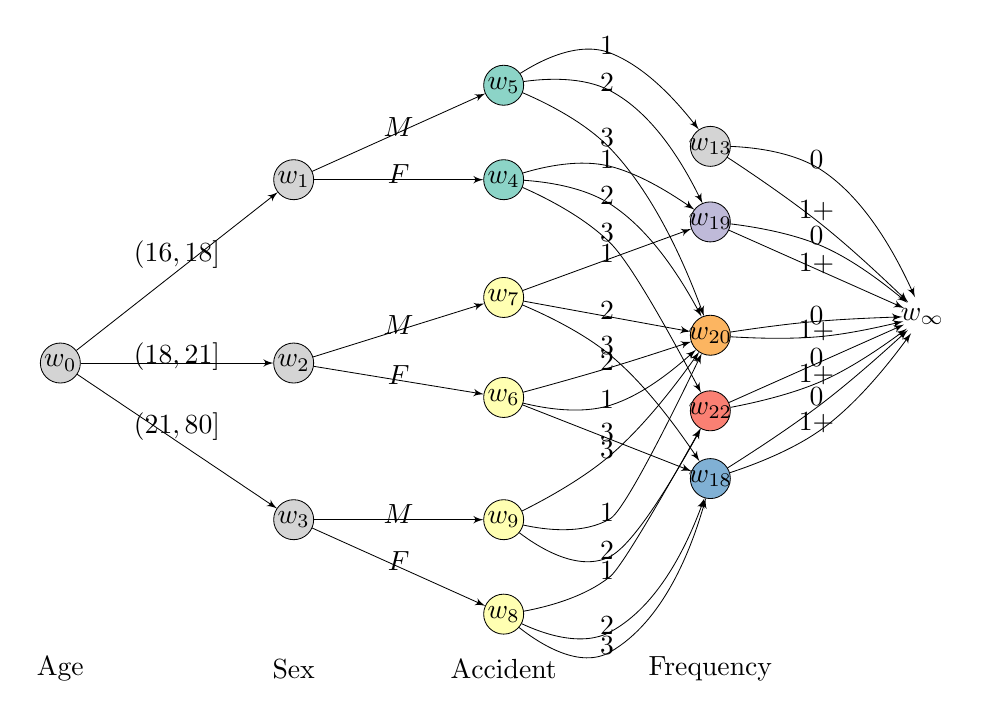
\begin{tikzpicture}[>=latex',line join=bevel, scale = 0.4]
  \pgfsetlinewidth{0.3bp}
%%
\pgfsetcolor{black}
  % Edge: v_{0} -> v_{1}
  \draw [->] (32.434bp,276.75bp) .. controls (68.487bp,305.07bp) and (162.67bp,379.08bp)  .. (213.74bp,419.2bp);
  \definecolor{strokecol}{rgb}{0.0,0.0,0.0};
  \pgfsetstrokecolor{strokecol}
  \draw (123.0bp,362.9bp) node {$(16,18]$};
  % Edge: v_{0} -> v_{2}
  \pgfsetcolor{black}
  \draw [->] (36.269bp,265.4bp) .. controls (72.974bp,265.4bp) and (155.9bp,265.4bp)  .. (209.92bp,265.4bp);
  \definecolor{strokecol}{rgb}{0.0,0.0,0.0};
  \pgfsetstrokecolor{strokecol}
  \draw (123.0bp,270.9bp) node {$(18,21]$};
  % Edge: v_{0} -> v_{3}
  \pgfsetcolor{black}
  \draw [->] (33.103bp,255.26bp) .. controls (69.276bp,230.98bp) and (161.09bp,169.33bp)  .. (213.03bp,134.45bp);
  \definecolor{strokecol}{rgb}{0.0,0.0,0.0};
  \pgfsetstrokecolor{strokecol}
  \draw (123.0bp,207.9bp) node {$(21,80]$};
  % Edge: v_{1} -> v_{4}
  \pgfsetcolor{black}
  \draw [->] (246.12bp,430.4bp) .. controls (279.14bp,430.4bp) and (349.33bp,430.4bp)  .. (398.93bp,430.4bp);
  \definecolor{strokecol}{rgb}{0.0,0.0,0.0};
  \pgfsetstrokecolor{strokecol}
  \draw (322.5bp,435.9bp) node {$F$};
  % Edge: v_{1} -> v_{5}
  \pgfsetcolor{black}
  \draw [->] (244.44bp,437.8bp) .. controls (277.39bp,452.62bp) and (351.73bp,486.05bp)  .. (400.46bp,507.97bp);
  \definecolor{strokecol}{rgb}{0.0,0.0,0.0};
  \pgfsetstrokecolor{strokecol}
  \draw (322.5bp,477.9bp) node {$M$};
  % Edge: v_{2} -> v_{6}
  \pgfsetcolor{black}
  \draw [->] (245.78bp,262.49bp) .. controls (278.78bp,257.08bp) and (349.71bp,245.44bp)  .. (399.13bp,237.34bp);
  \definecolor{strokecol}{rgb}{0.0,0.0,0.0};
  \pgfsetstrokecolor{strokecol}
  \draw (322.5bp,254.9bp) node {$F$};
  % Edge: v_{2} -> v_{7}
  \pgfsetcolor{black}
  \draw [->] (245.44bp,270.85bp) .. controls (278.49bp,281.17bp) and (350.46bp,303.63bp)  .. (399.6bp,318.97bp);
  \definecolor{strokecol}{rgb}{0.0,0.0,0.0};
  \pgfsetstrokecolor{strokecol}
  \draw (322.5bp,299.9bp) node {$M$};
  % Edge: v_{3} -> v_{8}
  \pgfsetcolor{black}
  \draw [->] (244.44bp,117.01bp) .. controls (277.39bp,102.19bp) and (351.73bp,68.757bp)  .. (400.46bp,46.842bp);
  \definecolor{strokecol}{rgb}{0.0,0.0,0.0};
  \pgfsetstrokecolor{strokecol}
  \draw (322.5bp,86.904bp) node {$F$};
  % Edge: v_{3} -> v_{9}
  \pgfsetcolor{black}
  \draw [->] (246.12bp,124.4bp) .. controls (279.14bp,124.4bp) and (349.33bp,124.4bp)  .. (398.93bp,124.4bp);
  \definecolor{strokecol}{rgb}{0.0,0.0,0.0};
  \pgfsetstrokecolor{strokecol}
  \draw (322.5bp,129.9bp) node {$M$};
  % Edge: v_{4} -> v_{19}
  \pgfsetcolor{black}
  \draw [->] (434.25bp,436.4bp) .. controls (453.66bp,442.28bp) and (486.01bp,449.4bp)  .. (513.0bp,442.4bp) .. controls (537.75bp,435.99bp) and (562.95bp,421.13bp)  .. (588.71bp,403.4bp);
  \definecolor{strokecol}{rgb}{0.0,0.0,0.0};
  \pgfsetstrokecolor{strokecol}
  \draw (510.0bp,448.9bp) node {$1$};
  % Edge: v_{4} -> v_{20}
  \pgfsetcolor{black}
  \draw [->] (435.04bp,429.88bp) .. controls (455.46bp,428.52bp) and (488.99bp,423.87bp)  .. (513.0bp,408.4bp) .. controls (548.65bp,385.44bp) and (575.66bp,343.23bp)  .. (595.1bp,307.06bp);
  \definecolor{strokecol}{rgb}{0.0,0.0,0.0};
  \pgfsetstrokecolor{strokecol}
  \draw (510.0bp,415.9bp) node {$2$};
  % Edge: v_{4} -> v_{22}
  \pgfsetcolor{black}
  \draw [->] (433.96bp,423.47bp) .. controls (454.59bp,414.39bp) and (489.54bp,396.82bp)  .. (513.0bp,373.4bp) .. controls (532.68bp,353.76bp) and (569.94bp,285.58bp)  .. (594.66bp,238.6bp);
  \definecolor{strokecol}{rgb}{0.0,0.0,0.0};
  \pgfsetstrokecolor{strokecol}
  \draw (510.0bp,382.9bp) node {$3$};
  % Edge: v_{5} -> v_{19}
  \pgfsetcolor{black}
  \draw [->] (434.8bp,518.73bp) .. controls (455.01bp,521.58bp) and (488.35bp,523.41bp)  .. (513.0bp,510.4bp) .. controls (550.91bp,490.39bp) and (577.56bp,446.55bp)  .. (596.0bp,409.03bp);
  \definecolor{strokecol}{rgb}{0.0,0.0,0.0};
  \pgfsetstrokecolor{strokecol}
  \draw (510.0bp,517.9bp) node {$2$};
  % Edge: v_{5} -> v_{20}
  \pgfsetcolor{black}
  \draw [->] (433.78bp,508.8bp) .. controls (454.54bp,499.94bp) and (489.95bp,482.49bp)  .. (513.0bp,458.4bp) .. controls (553.19bp,416.41bp) and (580.6bp,352.95bp)  .. (597.35bp,307.54bp);
  \definecolor{strokecol}{rgb}{0.0,0.0,0.0};
  \pgfsetstrokecolor{strokecol}
  \draw (510.0bp,467.9bp) node {$3$};
  % Edge: v_{5} -> v_{13}
  \pgfsetcolor{black}
  \draw [->] (431.89bp,526.06bp) .. controls (450.99bp,538.32bp) and (484.98bp,555.45bp)  .. (513.0bp,544.4bp) .. controls (543.8bp,532.27bp) and (570.27bp,504.07bp)  .. (592.63bp,475.5bp);
  \definecolor{strokecol}{rgb}{0.0,0.0,0.0};
  \pgfsetstrokecolor{strokecol}
  \draw (510.0bp,550.9bp) node {$1$};
  % Edge: v_{6} -> v_{20}
  \pgfsetcolor{black}
  \draw [->] (434.44bp,229.32bp) .. controls (454.03bp,224.48bp) and (486.54bp,219.06bp)  .. (513.0bp,227.4bp) .. controls (539.73bp,235.83bp) and (565.43bp,255.34bp)  .. (590.11bp,277.42bp);
  \definecolor{strokecol}{rgb}{0.0,0.0,0.0};
  \pgfsetstrokecolor{strokecol}
  \draw (510.0bp,232.9bp) node {$1$};
  % Edge: v_{6} -> v_{20}
  \pgfsetcolor{black}
  \draw [->] (434.4bp,239.09bp) .. controls (453.68bp,244.32bp) and (485.65bp,253.15bp)  .. (513.0bp,261.4bp) .. controls (534.28bp,267.82bp) and (558.23bp,275.57bp)  .. (585.81bp,284.65bp);
  \definecolor{strokecol}{rgb}{0.0,0.0,0.0};
  \pgfsetstrokecolor{strokecol}
  \draw (510.0bp,266.9bp) node {$2$};
  % Edge: v_{6} -> v_{18}
  \pgfsetcolor{black}
  \draw [->] (433.83bp,227.8bp) .. controls (466.26bp,215.07bp) and (537.6bp,187.07bp)  .. (586.07bp,168.05bp);
  \definecolor{strokecol}{rgb}{0.0,0.0,0.0};
  \pgfsetstrokecolor{strokecol}
  \draw (510.0bp,202.9bp) node {$3$};
  % Edge: v_{7} -> v_{19}
  \pgfsetcolor{black}
  \draw [->] (434.17bp,330.68bp) .. controls (466.69bp,342.57bp) and (537.51bp,368.46bp)  .. (585.88bp,386.14bp);
  \definecolor{strokecol}{rgb}{0.0,0.0,0.0};
  \pgfsetstrokecolor{strokecol}
  \draw (510.0bp,363.9bp) node {$1$};
  % Edge: v_{7} -> v_{20}
  \pgfsetcolor{black}
  \draw [->] (434.83bp,321.14bp) .. controls (467.33bp,315.2bp) and (536.4bp,302.58bp)  .. (585.22bp,293.65bp);
  \definecolor{strokecol}{rgb}{0.0,0.0,0.0};
  \pgfsetstrokecolor{strokecol}
  \draw (510.0bp,312.9bp) node {$2$};
  % Edge: v_{7} -> v_{18}
  \pgfsetcolor{black}
  \draw [->] (433.83bp,317.71bp) .. controls (454.01bp,309.17bp) and (488.21bp,292.99bp)  .. (513.0bp,272.4bp) .. controls (543.63bp,246.97bp) and (571.23bp,209.8bp)  .. (593.25bp,177.02bp);
  \definecolor{strokecol}{rgb}{0.0,0.0,0.0};
  \pgfsetstrokecolor{strokecol}
  \draw (510.0bp,280.9bp) node {$3$};
  % Edge: v_{8} -> v_{22}
  \pgfsetcolor{black}
  \draw [->] (435.07bp,42.042bp) .. controls (455.83bp,45.858bp) and (489.98bp,54.636bp)  .. (513.0bp,73.404bp) .. controls (523.95bp,82.331bp) and (566.93bp,157.73bp)  .. (594.25bp,206.6bp);
  \definecolor{strokecol}{rgb}{0.0,0.0,0.0};
  \pgfsetstrokecolor{strokecol}
  \draw (510.0bp,78.904bp) node {$1$};
  % Edge: v_{8} -> v_{18}
  \pgfsetcolor{black}
  \draw [->] (432.97bp,30.895bp) .. controls (452.89bp,21.542bp) and (487.45bp,9.5615bp)  .. (513.0bp,23.404bp) .. controls (556.31bp,46.862bp) and (582.07bp,101.2bp)  .. (597.67bp,143.78bp);
  \definecolor{strokecol}{rgb}{0.0,0.0,0.0};
  \pgfsetstrokecolor{strokecol}
  \draw (510.0bp,28.904bp) node {$2$};
  % Edge: v_{8} -> v_{18}
  \pgfsetcolor{black}
  \draw [->] (430.72bp,27.474bp) .. controls (449.98bp,12.25bp) and (485.75bp,-10.337bp)  .. (513.0bp,5.4039bp) .. controls (560.81bp,33.016bp) and (585.48bp,96.751bp)  .. (598.96bp,143.72bp);
  \definecolor{strokecol}{rgb}{0.0,0.0,0.0};
  \pgfsetstrokecolor{strokecol}
  \draw (510.0bp,10.904bp) node {$3$};
  % Edge: v_{9} -> v_{20}
  \pgfsetcolor{black}
  \draw [->] (434.36bp,119.65bp) .. controls (454.75bp,115.11bp) and (488.85bp,110.9bp)  .. (513.0bp,125.4bp) .. controls (526.29bp,133.39bp) and (569.48bp,220.52bp)  .. (595.27bp,274.1bp);
  \definecolor{strokecol}{rgb}{0.0,0.0,0.0};
  \pgfsetstrokecolor{strokecol}
  \draw (510.0bp,130.9bp) node {$1$};
  % Edge: v_{9} -> v_{20}
  \pgfsetcolor{black}
  \draw [->] (433.37bp,132.16bp) .. controls (453.39bp,142.12bp) and (487.74bp,160.71bp)  .. (513.0bp,182.4bp) .. controls (542.71bp,207.93bp) and (570.54bp,243.9bp)  .. (592.98bp,275.44bp);
  \definecolor{strokecol}{rgb}{0.0,0.0,0.0};
  \pgfsetstrokecolor{strokecol}
  \draw (510.0bp,187.9bp) node {$3$};
  % Edge: v_{9} -> v_{22}
  \pgfsetcolor{black}
  \draw [->] (430.9bp,112.77bp) .. controls (450.07bp,98.213bp) and (485.39bp,76.877bp)  .. (513.0bp,91.404bp) .. controls (534.87bp,102.91bp) and (570.21bp,162.47bp)  .. (594.43bp,206.26bp);
  \definecolor{strokecol}{rgb}{0.0,0.0,0.0};
  \pgfsetstrokecolor{strokecol}
  \draw (510.0bp,96.904bp) node {$2$};
  % Edge: v_{19} -> w_inf
  \pgfsetcolor{black}
  \draw [->] (621.18bp,390.63bp) .. controls (641.93bp,388.12bp) and (676.55bp,382.42bp)  .. (704.0bp,370.4bp) .. controls (729.53bp,359.23bp) and (755.23bp,340.29bp)  .. (780.41bp,319.55bp);
  \definecolor{strokecol}{rgb}{0.0,0.0,0.0};
  \pgfsetstrokecolor{strokecol}
  \draw (698.5bp,379.9bp) node {$0$};
  % Edge: v_{19} -> w_inf
  \pgfsetcolor{black}
  \draw [->] (619.62bp,385.01bp) .. controls (652.92bp,370.19bp) and (728.04bp,336.76bp)  .. (777.29bp,314.84bp);
  \definecolor{strokecol}{rgb}{0.0,0.0,0.0};
  \pgfsetstrokecolor{strokecol}
  \draw (698.5bp,354.9bp) node {$1+$};
  % Edge: v_{20} -> w_inf
  \pgfsetcolor{black}
  \draw [->] (620.88bp,293.23bp) .. controls (639.01bp,296.0bp) and (667.88bp,300.11bp)  .. (693.0bp,302.4bp) .. controls (717.45bp,304.64bp) and (745.33bp,305.92bp)  .. (775.72bp,306.96bp);
  \definecolor{strokecol}{rgb}{0.0,0.0,0.0};
  \pgfsetstrokecolor{strokecol}
  \draw (698.5bp,307.9bp) node {$0$};
  % Edge: v_{20} -> w_inf
  \pgfsetcolor{black}
  \draw [->] (621.3bp,289.03bp) .. controls (641.57bp,287.79bp) and (675.21bp,286.55bp)  .. (704.0bp,289.4bp) .. controls (725.14bp,291.5bp) and (748.67bp,296.29bp)  .. (776.56bp,302.85bp);
  \definecolor{strokecol}{rgb}{0.0,0.0,0.0};
  \pgfsetstrokecolor{strokecol}
  \draw (698.5bp,294.9bp) node {$1+$};
  % Edge: v_{22} -> w_inf
  \pgfsetcolor{black}
  \draw [->] (619.62bp,229.8bp) .. controls (652.92bp,244.62bp) and (728.04bp,278.05bp)  .. (777.29bp,299.97bp);
  \definecolor{strokecol}{rgb}{0.0,0.0,0.0};
  \pgfsetstrokecolor{strokecol}
  \draw (698.5bp,269.9bp) node {$0$};
  % Edge: v_{22} -> w_inf
  \pgfsetcolor{black}
  \draw [->] (621.08bp,225.48bp) .. controls (641.75bp,229.38bp) and (676.28bp,237.13bp)  .. (704.0bp,249.4bp) .. controls (728.46bp,260.23bp) and (753.86bp,277.22bp)  .. (779.83bp,296.27bp);
  \definecolor{strokecol}{rgb}{0.0,0.0,0.0};
  \pgfsetstrokecolor{strokecol}
  \draw (698.5bp,254.9bp) node {$1+$};
  % Edge: v_{13} -> w_inf
  \pgfsetcolor{black}
  \draw [->] (621.34bp,460.37bp) .. controls (642.87bp,459.49bp) and (678.83bp,455.32bp)  .. (704.0bp,438.4bp) .. controls (742.48bp,412.55bp) and (769.22bp,364.21bp)  .. (787.24bp,324.55bp);
  \definecolor{strokecol}{rgb}{0.0,0.0,0.0};
  \pgfsetstrokecolor{strokecol}
  \draw (698.5bp,448.9bp) node {$0$};
  % Edge: v_{13} -> w_inf
  \pgfsetcolor{black}
  \draw [->] (618.15bp,450.62bp) .. controls (638.28bp,437.43bp) and (674.74bp,412.87bp)  .. (704.0bp,389.4bp) .. controls (728.88bp,369.45bp) and (755.7bp,344.53bp)  .. (781.05bp,320.17bp);
  \definecolor{strokecol}{rgb}{0.0,0.0,0.0};
  \pgfsetstrokecolor{strokecol}
  \draw (698.5bp,402.9bp) node {$1+$};
  % Edge: v_{18} -> w_inf
  \pgfsetcolor{black}
  \draw [->] (618.46bp,170.98bp) .. controls (638.63bp,183.67bp) and (674.79bp,207.05bp)  .. (704.0bp,229.4bp) .. controls (728.63bp,248.26bp) and (755.3bp,271.8bp)  .. (780.71bp,294.98bp);
  \definecolor{strokecol}{rgb}{0.0,0.0,0.0};
  \pgfsetstrokecolor{strokecol}
  \draw (698.5bp,234.9bp) node {$0$};
  % Edge: v_{18} -> w_inf
  \pgfsetcolor{black}
  \draw [->] (620.24bp,166.59bp) .. controls (641.34bp,173.47bp) and (677.5bp,187.04bp)  .. (704.0bp,206.4bp) .. controls (733.97bp,228.3bp) and (761.23bp,261.65bp)  .. (783.68bp,292.22bp);
  \definecolor{strokecol}{rgb}{0.0,0.0,0.0};
  \pgfsetstrokecolor{strokecol}
  \draw (698.5bp,211.9bp) node {$1+$};
  % Node: v_{0}
\begin{scope}
  \definecolor{strokecol}{rgb}{0.0,0.0,0.0};
  \pgfsetstrokecolor{strokecol}
  \definecolor{fillcol}{rgb}{0.83,0.83,0.83};
  \pgfsetfillcolor{fillcol}
  \filldraw [opacity=1] (18.0bp,265.4bp) ellipse (18.0bp and 18.0bp);
  \draw (18.0bp,265.4bp) node {$w_{0}$};
\end{scope}
  % Node: v_{1}
\begin{scope}
  \definecolor{strokecol}{rgb}{0.0,0.0,0.0};
  \pgfsetstrokecolor{strokecol}
  \definecolor{fillcol}{rgb}{0.83,0.83,0.83};
  \pgfsetfillcolor{fillcol}
  \filldraw [opacity=1] (228.0bp,430.4bp) ellipse (18.0bp and 18.0bp);
  \draw (228.0bp,430.4bp) node {$w_{1}$};
\end{scope}
  % Node: v_{2}
\begin{scope}
  \definecolor{strokecol}{rgb}{0.0,0.0,0.0};
  \pgfsetstrokecolor{strokecol}
  \definecolor{fillcol}{rgb}{0.83,0.83,0.83};
  \pgfsetfillcolor{fillcol}
  \filldraw [opacity=1] (228.0bp,265.4bp) ellipse (18.0bp and 18.0bp);
  \draw (228.0bp,265.4bp) node {$w_{2}$};
\end{scope}
  % Node: v_{3}
\begin{scope}
  \definecolor{strokecol}{rgb}{0.0,0.0,0.0};
  \pgfsetstrokecolor{strokecol}
  \definecolor{fillcol}{rgb}{0.83,0.83,0.83};
  \pgfsetfillcolor{fillcol}
  \filldraw [opacity=1] (228.0bp,124.4bp) ellipse (18.0bp and 18.0bp);
  \draw (228.0bp,124.4bp) node {$w_{3}$};
\end{scope}
  % Node: v_{4}
\begin{scope}
  \definecolor{strokecol}{rgb}{0.0,0.0,0.0};
  \pgfsetstrokecolor{strokecol}
  \definecolor{fillcol}{rgb}{0.55,0.83,0.78};
  \pgfsetfillcolor{fillcol}
  \filldraw [opacity=1] (417.0bp,430.4bp) ellipse (18.0bp and 18.0bp);
  \draw (417.0bp,430.4bp) node {$w_{4}$};
\end{scope}
  % Node: v_{5}
\begin{scope}
  \definecolor{strokecol}{rgb}{0.0,0.0,0.0};
  \pgfsetstrokecolor{strokecol}
  \definecolor{fillcol}{rgb}{0.55,0.83,0.78};
  \pgfsetfillcolor{fillcol}
  \filldraw [opacity=1] (417.0bp,515.4bp) ellipse (18.0bp and 18.0bp);
  \draw (417.0bp,515.4bp) node {$w_{5}$};
\end{scope}
  % Node: v_{6}
\begin{scope}
  \definecolor{strokecol}{rgb}{0.0,0.0,0.0};
  \pgfsetstrokecolor{strokecol}
  \definecolor{fillcol}{rgb}{1.0,1.0,0.7};
  \pgfsetfillcolor{fillcol}
  \filldraw [opacity=1] (417.0bp,234.4bp) ellipse (18.0bp and 18.0bp);
  \draw (417.0bp,234.4bp) node {$w_{6}$};
\end{scope}
  % Node: v_{7}
\begin{scope}
  \definecolor{strokecol}{rgb}{0.0,0.0,0.0};
  \pgfsetstrokecolor{strokecol}
  \definecolor{fillcol}{rgb}{1.0,1.0,0.7};
  \pgfsetfillcolor{fillcol}
  \filldraw [opacity=1] (417.0bp,324.4bp) ellipse (18.0bp and 18.0bp);
  \draw (417.0bp,324.4bp) node {$w_{7}$};
\end{scope}
  % Node: v_{8}
\begin{scope}
  \definecolor{strokecol}{rgb}{0.0,0.0,0.0};
  \pgfsetstrokecolor{strokecol}
  \definecolor{fillcol}{rgb}{1.0,1.0,0.7};
  \pgfsetfillcolor{fillcol}
  \filldraw [opacity=1] (417.0bp,39.4bp) ellipse (18.0bp and 18.0bp);
  \draw (417.0bp,39.404bp) node {$w_{8}$};
\end{scope}
  % Node: v_{9}
\begin{scope}
  \definecolor{strokecol}{rgb}{0.0,0.0,0.0};
  \pgfsetstrokecolor{strokecol}
  \definecolor{fillcol}{rgb}{1.0,1.0,0.7};
  \pgfsetfillcolor{fillcol}
  \filldraw [opacity=1] (417.0bp,124.4bp) ellipse (18.0bp and 18.0bp);
  \draw (417.0bp,124.4bp) node {$w_{9}$};
\end{scope}
  % Node: v_{19}
\begin{scope}
  \definecolor{strokecol}{rgb}{0.0,0.0,0.0};
  \pgfsetstrokecolor{strokecol}
  \definecolor{fillcol}{rgb}{0.75,0.73,0.85};
  \pgfsetfillcolor{fillcol}
  \filldraw [opacity=1] (603.0bp,392.4bp) ellipse (18.0bp and 18.0bp);
  \draw (603.0bp,392.4bp) node {$w_{19}$};
\end{scope}
  % Node: v_{20}
\begin{scope}
  \definecolor{strokecol}{rgb}{0.0,0.0,0.0};
  \pgfsetstrokecolor{strokecol}
  \definecolor{fillcol}{rgb}{0.99,0.71,0.38};
  \pgfsetfillcolor{fillcol}
  \filldraw [opacity=1] (603.0bp,290.4bp) ellipse (18.0bp and 18.0bp);
  \draw (603.0bp,290.4bp) node {$w_{20}$};
\end{scope}
  % Node: v_{22}
\begin{scope}
  \definecolor{strokecol}{rgb}{0.0,0.0,0.0};
  \pgfsetstrokecolor{strokecol}
  \definecolor{fillcol}{rgb}{0.98,0.5,0.45};
  \pgfsetfillcolor{fillcol}
  \filldraw [opacity=1] (603.0bp,222.4bp) ellipse (18.0bp and 18.0bp);
  \draw (603.0bp,222.4bp) node {$w_{22}$};
\end{scope}
  % Node: v_{13}
\begin{scope}
  \definecolor{strokecol}{rgb}{0.0,0.0,0.0};
  \pgfsetstrokecolor{strokecol}
  \definecolor{fillcol}{rgb}{0.83,0.83,0.83};
  \pgfsetfillcolor{fillcol}
  \filldraw [opacity=1] (603.0bp,460.4bp) ellipse (18.0bp and 18.0bp);
  \draw (603.0bp,460.4bp) node {$w_{13}$};
\end{scope}
  % Node: v_{18}
\begin{scope}
  \definecolor{strokecol}{rgb}{0.0,0.0,0.0};
  \pgfsetstrokecolor{strokecol}
  \definecolor{fillcol}{rgb}{0.5,0.69,0.83};
  \pgfsetfillcolor{fillcol}
  \filldraw [opacity=1] (603.0bp,161.4bp) ellipse (18.0bp and 18.0bp);
  \draw (603.0bp,161.4bp) node {$w_{18}$};
\end{scope}
  % Node: w_inf
\begin{scope}
  \definecolor{strokecol}{rgb}{0.0,0.0,0.0};
  \pgfsetstrokecolor{strokecol}
  \draw (794.0bp,307.4bp) node {$w_\infty$};
\end{scope}

\begin{scope}
  \draw (18.0bp,-10bp) node {Age};
  \draw (228.0bp,-10bp) node {Sex};
  \draw (603.0bp,-10bp) node {Frequency};
  \draw (417.0bp,-10bp) node {Accident};
\end{scope}
%
\end{tikzpicture}
\caption{CEG derived from the staged tree in Fig~\ref{stagedtree} (colours only applied to positions which include more than one node of the underlying staged tree, otherwise grey).}
\label{ceg:freq-acc}
\end{figure}
The predictive probabilities of an accident associated with the positions $w_{13}, w_{19}, w_{20}, w_{22}, w_{18}$ in the final layer of the CEG are: 13.6\%, 9.6\%, 6.5\%, 4.2\%, 1.9\% respectively.
The ordinal CEG allows us to immediately identify the groups of respondents with highest accident liability: young men aged 16-18 driving everyday. Similarly, the group with second highest accident liability are men aged 16-18 driving 4-6 days per week, men aged 18-21 driving everyday and females aged 16-18 driving everyday. Another advantage of the ordinal CEG is that we can immediately tell that overall Male respondents are associated with higher risk of non-low speed accidents than Female respondents and that the younger groups of respondents ere associated with higher accident risk than older groups. Similar and perhaps more precise conclusions could be made by examining the coefficients of a generalised linear model, yet the CEG representation provides us with a framework for presenting these conclusions without having to rely on quantitative measures. 

\subsection{Missing values}\label{subsec:missing}
In the previous section we constructed a CEG model which allows us to categorise the drivers into a groups of increasing accident liability. We used three explanatory variables: age, sex and frequency. Instead of the frequency as a measure of exposure to road accidents we may instead rely on the reported mileage. However, out of the 9491 observations considered for this model 757 have a missing response to the question about the mileage. We may simply discard those observations and rely only on the remaining complete responses, yet CEGs allow us to not only include the incomplete observations into the model, but also to reason about the patterns of the missingness. For a more detailed discussion on the CEG models of missingness refer to \cite{barclay2014missingness}. 

As previously, let $X_a$ describe the age, $X_s$ sex, and $Y$ the accident involvement during the first 6 months after passing the test. Let also $X_m$ describe the annualised mileage taking one of the three values coded as:  1 = above 12000, 2 = 4000 - 12000 miles, 3 = below 4000 miles. We further introduce a new variable $R_m$ indicating whether $X_m$ is missing or not. Fig~\ref{ceg:mis-miles} presents the most probable CEG found by the AHC algorithm on $\boldsymbol{X} = (X_a, X_s, R_m, X_m, Y)$. The positions $w_{27}, w_{29}, w_{48}, w_{19}$ in the final layer of the CEG are ordered with respect to the predictive probability of being involved in an accident: 14.1\%, 8.6\%, 4.9\%, 2.7\%, respectively.
\begin{figure}
\centering
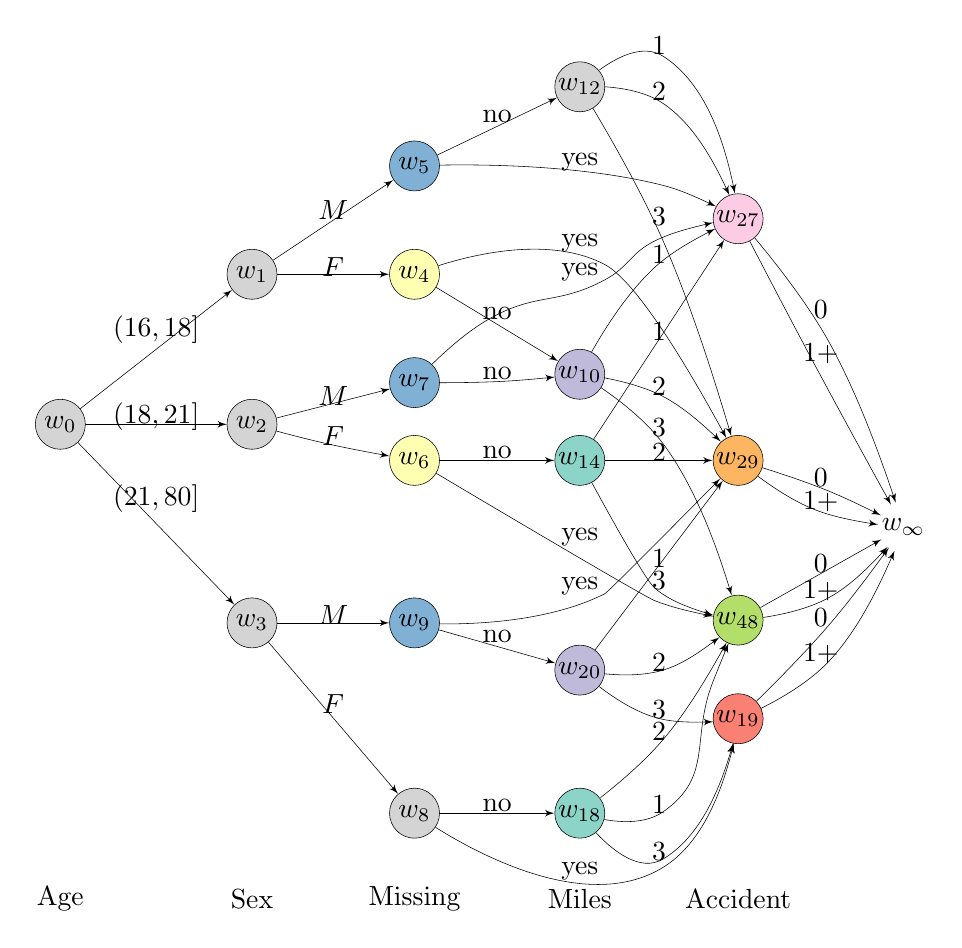
\begin{tikzpicture}[>=latex',line join=bevel, scale = 0.5]
  \pgfsetlinewidth{0.2bp}
%%
\pgfsetcolor{black}
  % Edge: w_{0} -> w_{1}
  \draw [->] (32.249bp,342.67bp) .. controls (56.214bp,361.43bp) and (104.77bp,399.43bp)  .. (141.62bp,428.27bp);
  \definecolor{strokecol}{rgb}{0.0,0.0,0.0};
  \pgfsetstrokecolor{strokecol}
  \draw (87.0bp,400.02bp) node {$(16,18]$};
  % Edge: w_{0} -> w_{2}
  \pgfsetcolor{black}
  \draw [->] (36.041bp,331.52bp) .. controls (59.389bp,331.52bp) and (100.33bp,331.52bp)  .. (137.95bp,331.52bp);
  \definecolor{strokecol}{rgb}{0.0,0.0,0.0};
  \pgfsetstrokecolor{strokecol}
  \draw (87.0bp,337.02bp) node {$(18,21]$};
  % Edge: w_{0} -> w_{3}
  \pgfsetcolor{black}
  \draw [->] (30.735bp,318.32bp) .. controls (54.868bp,293.31bp) and (107.41bp,238.86bp)  .. (143.3bp,201.68bp);
  \definecolor{strokecol}{rgb}{0.0,0.0,0.0};
  \pgfsetstrokecolor{strokecol}
  \draw (87.0bp,278.02bp) node {$(21,80]$};
  % Edge: w_{1} -> w_{4}
  \pgfsetcolor{black}
  \draw [->] (174.02bp,439.52bp) .. controls (192.86bp,439.52bp) and (222.69bp,439.52bp)  .. (254.76bp,439.52bp);
  \definecolor{strokecol}{rgb}{0.0,0.0,0.0};
  \pgfsetstrokecolor{strokecol}
  \draw (214.5bp,445.02bp) node {$F$};
  % Edge: w_{1} -> w_{5}
  \pgfsetcolor{black}
  \draw [->] (171.3bp,449.72bp) .. controls (191.09bp,462.91bp) and (225.8bp,486.05bp)  .. (257.7bp,507.32bp);
  \definecolor{strokecol}{rgb}{0.0,0.0,0.0};
  \pgfsetstrokecolor{strokecol}
  \draw (214.5bp,486.02bp) node {$M$};
  % Edge: w_{2} -> w_{6}
  \pgfsetcolor{black}
  \draw [->] (173.44bp,326.69bp) .. controls (183.98bp,323.85bp) and (197.72bp,320.28bp)  .. (210.0bp,317.52bp) .. controls (221.44bp,314.95bp) and (234.14bp,312.46bp)  .. (255.01bp,308.62bp);
  \definecolor{strokecol}{rgb}{0.0,0.0,0.0};
  \pgfsetstrokecolor{strokecol}
  \draw (214.5bp,323.02bp) node {$F$};
  % Edge: w_{2} -> w_{7}
  \pgfsetcolor{black}
  \draw [->] (173.52bp,336.01bp) .. controls (192.56bp,340.89bp) and (223.24bp,348.76bp)  .. (255.36bp,357.0bp);
  \definecolor{strokecol}{rgb}{0.0,0.0,0.0};
  \pgfsetstrokecolor{strokecol}
  \draw (214.5bp,352.02bp) node {$M$};
  % Edge: w_{3} -> w_{8}
  \pgfsetcolor{black}
  \draw [->] (167.86bp,174.63bp) .. controls (188.27bp,150.73bp) and (230.18bp,101.66bp)  .. (261.11bp,65.446bp);
  \definecolor{strokecol}{rgb}{0.0,0.0,0.0};
  \pgfsetstrokecolor{strokecol}
  \draw (214.5bp,130.02bp) node {$F$};
  % Edge: w_{3} -> w_{9}
  \pgfsetcolor{black}
  \draw [->] (174.02bp,188.52bp) .. controls (192.86bp,188.52bp) and (222.69bp,188.52bp)  .. (254.76bp,188.52bp);
  \definecolor{strokecol}{rgb}{0.0,0.0,0.0};
  \pgfsetstrokecolor{strokecol}
  \draw (214.5bp,194.02bp) node {$M$};
  % Edge: w_{4} -> w_{10}
  \pgfsetcolor{black}
  \draw [->] (288.56bp,430.11bp) .. controls (308.69bp,417.92bp) and (343.99bp,396.57bp)  .. (376.44bp,376.93bp);
  \definecolor{strokecol}{rgb}{0.0,0.0,0.0};
  \pgfsetstrokecolor{strokecol}
  \draw (332.5bp,411.02bp) node {no};
  % Edge: w_{4} -> w_{29}
  \pgfsetcolor{black}
  \draw [->] (290.22bp,445.73bp) .. controls (317.44bp,454.43bp) and (371.26bp,467.01bp)  .. (410.0bp,446.52bp) .. controls (433.85bp,433.9bp) and (472.39bp,367.81bp)  .. (497.58bp,321.58bp);
  \definecolor{strokecol}{rgb}{0.0,0.0,0.0};
  \pgfsetstrokecolor{strokecol}
  \draw (392.0bp,462.02bp) node {yes};
  % Edge: w_{5} -> w_{12}
  \pgfsetcolor{black}
  \draw [->] (289.55bp,525.44bp) .. controls (309.44bp,534.97bp) and (343.05bp,551.07bp)  .. (375.59bp,566.66bp);
  \definecolor{strokecol}{rgb}{0.0,0.0,0.0};
  \pgfsetstrokecolor{strokecol}
  \draw (332.5bp,553.02bp) node {no};
  % Edge: w_{5} -> w_{27}
  \pgfsetcolor{black}
  \draw [->] (291.11bp,518.11bp) .. controls (323.8bp,518.73bp) and (394.59bp,518.06bp)  .. (452.0bp,503.52bp) .. controls (461.79bp,501.04bp) and (472.03bp,496.92bp)  .. (489.98bp,488.38bp);
  \definecolor{strokecol}{rgb}{0.0,0.0,0.0};
  \pgfsetstrokecolor{strokecol}
  \draw (392.0bp,520.02bp) node {yes};
  % Edge: w_{6} -> w_{14}
  \pgfsetcolor{black}
  \draw [->] (291.07bp,305.52bp) .. controls (310.29bp,305.52bp) and (340.97bp,305.52bp)  .. (373.76bp,305.52bp);
  \definecolor{strokecol}{rgb}{0.0,0.0,0.0};
  \pgfsetstrokecolor{strokecol}
  \draw (332.5bp,311.02bp) node {no};
  % Edge: w_{6} -> w_{48}
  \pgfsetcolor{black}
  \draw [->] (288.67bp,296.2bp) .. controls (329.69bp,271.83bp) and (437.64bp,207.85bp)  .. (446.0bp,204.52bp) .. controls (456.1bp,200.5bp) and (467.65bp,197.46bp)  .. (487.98bp,193.27bp);
  \definecolor{strokecol}{rgb}{0.0,0.0,0.0};
  \pgfsetstrokecolor{strokecol}
  \draw (392.0bp,250.02bp) node {yes};
  % Edge: w_{7} -> w_{10}
  \pgfsetcolor{black}
  \draw [->] (291.22bp,361.42bp) .. controls (304.26bp,361.45bp) and (322.22bp,361.67bp)  .. (338.0bp,362.52bp) .. controls (346.46bp,362.97bp) and (355.65bp,363.73bp)  .. (374.03bp,365.51bp);
  \definecolor{strokecol}{rgb}{0.0,0.0,0.0};
  \pgfsetstrokecolor{strokecol}
  \draw (332.5bp,368.02bp) node {no};
  % Edge: w_{7} -> w_{27}
  \pgfsetcolor{black}
  \draw [->] (285.68bp,374.79bp) .. controls (295.99bp,384.94bp) and (311.36bp,398.66bp)  .. (327.0bp,407.52bp) .. controls (360.87bp,426.71bp) and (375.71bp,417.09bp)  .. (410.0bp,435.52bp) .. controls (427.85bp,445.12bp) and (427.84bp,454.51bp)  .. (446.0bp,463.52bp) .. controls (455.99bp,468.48bp) and (467.71bp,472.05bp)  .. (488.0bp,476.67bp);
  \definecolor{strokecol}{rgb}{0.0,0.0,0.0};
  \pgfsetstrokecolor{strokecol}
  \draw (392.0bp,441.02bp) node {yes};
  % Edge: w_{8} -> w_{18}
  \pgfsetcolor{black}
  \draw [->] (291.07bp,51.519bp) .. controls (310.29bp,51.519bp) and (340.97bp,51.519bp)  .. (373.76bp,51.519bp);
  \definecolor{strokecol}{rgb}{0.0,0.0,0.0};
  \pgfsetstrokecolor{strokecol}
  \draw (332.5bp,57.019bp) node {no};
  % Edge: w_{8} -> w_{19}
  \pgfsetcolor{black}
  \draw [->] (288.14bp,41.337bp) .. controls (320.62bp,20.892bp) and (398.37bp,-20.489bp)  .. (452.0bp,12.519bp) .. controls (479.88bp,29.677bp) and (493.89bp,66.157bp)  .. (502.89bp,101.6bp);
  \definecolor{strokecol}{rgb}{0.0,0.0,0.0};
  \pgfsetstrokecolor{strokecol}
  \draw (392.0bp,10.019bp) node {yes};
  % Edge: w_{9} -> w_{29}
  \pgfsetcolor{black}
  \draw [->] (291.38bp,187.8bp) .. controls (318.75bp,187.49bp) and (371.14bp,189.84bp)  .. (410.0bp,209.52bp) .. controls (412.35bp,210.71bp) and (458.43bp,257.25bp)  .. (493.08bp,292.39bp);
  \definecolor{strokecol}{rgb}{0.0,0.0,0.0};
  \pgfsetstrokecolor{strokecol}
  \draw (392.0bp,215.02bp) node {yes};
  % Edge: w_{9} -> w_{20}
  \pgfsetcolor{black}
  \draw [->] (290.56bp,183.5bp) .. controls (310.07bp,177.93bp) and (341.82bp,168.86bp)  .. (374.37bp,159.56bp);
  \definecolor{strokecol}{rgb}{0.0,0.0,0.0};
  \pgfsetstrokecolor{strokecol}
  \draw (332.5bp,179.02bp) node {no};
  % Edge: w_{10} -> w_{29}
  \pgfsetcolor{black}
  \draw [->] (409.83bp,364.91bp) .. controls (422.18bp,362.6bp) and (438.73bp,358.48bp)  .. (452.0bp,351.52bp) .. controls (464.44bp,344.99bp) and (476.51bp,335.15bp)  .. (493.48bp,319.07bp);
  \definecolor{strokecol}{rgb}{0.0,0.0,0.0};
  \pgfsetstrokecolor{strokecol}
  \draw (449.0bp,359.02bp) node {$2$};
  % Edge: w_{10} -> w_{27}
  \pgfsetcolor{black}
  \draw [->] (400.45bp,383.49bp) .. controls (409.88bp,400.21bp) and (426.41bp,426.5bp)  .. (446.0bp,444.52bp) .. controls (456.12bp,453.83bp) and (469.14bp,461.79bp)  .. (489.46bp,472.29bp);
  \definecolor{strokecol}{rgb}{0.0,0.0,0.0};
  \pgfsetstrokecolor{strokecol}
  \draw (449.0bp,454.02bp) node {$1$};
  % Edge: w_{10} -> w_{48}
  \pgfsetcolor{black}
  \draw [->] (407.31bp,357.84bp) .. controls (420.61bp,348.78bp) and (439.63bp,334.17bp)  .. (452.0bp,317.52bp) .. controls (474.81bp,286.82bp) and (490.17bp,245.04bp)  .. (501.35bp,208.3bp);
  \definecolor{strokecol}{rgb}{0.0,0.0,0.0};
  \pgfsetstrokecolor{strokecol}
  \draw (449.0bp,329.02bp) node {$3$};
  % Edge: w_{29} -> w_inf
  \pgfsetcolor{black}
  \draw [->] (523.32bp,300.29bp) .. controls (536.54bp,296.15bp) and (555.12bp,290.0bp)  .. (571.0bp,283.52bp) .. controls (580.48bp,279.65bp) and (590.65bp,274.91bp)  .. (608.69bp,266.02bp);
  \definecolor{strokecol}{rgb}{0.0,0.0,0.0};
  \pgfsetstrokecolor{strokecol}
  \draw (565.5bp,293.02bp) node {$0$};
  % Edge: w_{29} -> w_inf
  \pgfsetcolor{black}
  \draw [->] (520.29bp,294.1bp) .. controls (530.72bp,286.33bp) and (545.51bp,276.41bp)  .. (560.0bp,270.52bp) .. controls (571.59bp,265.81bp) and (585.06bp,262.75bp)  .. (606.82bp,259.29bp);
  \definecolor{strokecol}{rgb}{0.0,0.0,0.0};
  \pgfsetstrokecolor{strokecol}
  \draw (565.5bp,276.02bp) node {$1+$};
  % Edge: w_{12} -> w_{29}
  \pgfsetcolor{black}
  \draw [->] (401.39bp,559.12bp) .. controls (413.98bp,538.06bp) and (436.55bp,498.84bp)  .. (452.0bp,463.52bp) .. controls (471.52bp,418.9bp) and (488.68bp,364.79bp)  .. (501.08bp,322.94bp);
  \definecolor{strokecol}{rgb}{0.0,0.0,0.0};
  \pgfsetstrokecolor{strokecol}
  \draw (449.0bp,481.02bp) node {$3$};
  % Edge: w_{12} -> w_{27}
  \pgfsetcolor{black}
  \draw [->] (406.13bp,586.6bp) .. controls (418.82bp,595.9bp) and (437.61bp,605.73bp)  .. (452.0bp,596.52bp) .. controls (482.41bp,577.06bp) and (495.94bp,535.64bp)  .. (503.67bp,497.69bp);
  \definecolor{strokecol}{rgb}{0.0,0.0,0.0};
  \pgfsetstrokecolor{strokecol}
  \draw (449.0bp,604.02bp) node {$1$};
  % Edge: w_{12} -> w_{27}
  \pgfsetcolor{black}
  \draw [->] (410.21bp,574.5bp) .. controls (422.9bp,573.67bp) and (439.69bp,570.86bp)  .. (452.0bp,562.52bp) .. controls (472.36bp,548.72bp) and (486.83bp,524.42bp)  .. (499.72bp,496.45bp);
  \definecolor{strokecol}{rgb}{0.0,0.0,0.0};
  \pgfsetstrokecolor{strokecol}
  \draw (449.0bp,571.02bp) node {$2$};
  % Edge: w_{27} -> w_inf
  \pgfsetcolor{black}
  \draw [->] (517.99bp,465.64bp) .. controls (532.03bp,448.91bp) and (555.34bp,419.54bp)  .. (571.0bp,391.52bp) .. controls (590.64bp,356.38bp) and (606.88bp,312.63bp)  .. (619.51bp,275.08bp);
  \definecolor{strokecol}{rgb}{0.0,0.0,0.0};
  \pgfsetstrokecolor{strokecol}
  \draw (565.5bp,414.02bp) node {$0$};
  % Edge: w_{27} -> w_inf
  \pgfsetcolor{black}
  \draw [->] (514.33bp,463.42bp) .. controls (524.87bp,443.11bp) and (543.61bp,407.14bp)  .. (560.0bp,376.52bp) .. controls (577.46bp,343.9bp) and (597.97bp,306.49bp)  .. (616.08bp,273.64bp);
  \definecolor{strokecol}{rgb}{0.0,0.0,0.0};
  \pgfsetstrokecolor{strokecol}
  \draw (565.5bp,382.02bp) node {$1+$};
  % Edge: w_{14} -> w_{29}
  \pgfsetcolor{black}
  \draw [->] (410.06bp,305.52bp) .. controls (428.22bp,305.52bp) and (456.46bp,305.52bp)  .. (487.64bp,305.52bp);
  \definecolor{strokecol}{rgb}{0.0,0.0,0.0};
  \pgfsetstrokecolor{strokecol}
  \draw (449.0bp,311.02bp) node {$2$};
  % Edge: w_{14} -> w_{27}
  \pgfsetcolor{black}
  \draw [->] (401.92bp,320.66bp) .. controls (421.79bp,350.99bp) and (466.63bp,419.43bp)  .. (496.02bp,464.29bp);
  \definecolor{strokecol}{rgb}{0.0,0.0,0.0};
  \pgfsetstrokecolor{strokecol}
  \draw (449.0bp,398.02bp) node {$1$};
  % Edge: w_{14} -> w_{48}
  \pgfsetcolor{black}
  \draw [->] (400.65bp,289.49bp) .. controls (414.17bp,264.64bp) and (439.47bp,219.06bp)  .. (446.0bp,213.52bp) .. controls (455.25bp,205.68bp) and (467.47bp,200.35bp)  .. (488.09bp,194.05bp);
  \definecolor{strokecol}{rgb}{0.0,0.0,0.0};
  \pgfsetstrokecolor{strokecol}
  \draw (449.0bp,219.02bp) node {$3$};
  % Edge: w_{48} -> w_inf
  \pgfsetcolor{black}
  \draw [->] (522.05bp,199.55bp) .. controls (542.12bp,210.86bp) and (576.7bp,230.33bp)  .. (609.21bp,248.63bp);
  \definecolor{strokecol}{rgb}{0.0,0.0,0.0};
  \pgfsetstrokecolor{strokecol}
  \draw (565.5bp,231.02bp) node {$0$};
  % Edge: w_{48} -> w_inf
  \pgfsetcolor{black}
  \draw [->] (524.0bp,192.43bp) .. controls (537.58bp,194.45bp) and (556.31bp,198.51bp)  .. (571.0bp,206.52bp) .. controls (584.53bp,213.9bp) and (597.2bp,225.5bp)  .. (613.63bp,243.29bp);
  \definecolor{strokecol}{rgb}{0.0,0.0,0.0};
  \pgfsetstrokecolor{strokecol}
  \draw (565.5bp,212.02bp) node {$1+$};
  % Edge: w_{18} -> w_{48}
  \pgfsetcolor{black}
  \draw [->] (409.62bp,46.937bp) .. controls (422.5bp,44.663bp) and (439.8bp,43.974bp)  .. (452.0bp,52.519bp) .. controls (488.65bp,78.178bp) and (471.53bp,104.92bp)  .. (488.0bp,146.52bp) .. controls (490.3bp,152.32bp) and (492.81bp,158.53bp)  .. (499.07bp,173.84bp);
  \definecolor{strokecol}{rgb}{0.0,0.0,0.0};
  \pgfsetstrokecolor{strokecol}
  \draw (449.0bp,58.019bp) node {$1$};
  % Edge: w_{18} -> w_{48}
  \pgfsetcolor{black}
  \draw [->] (406.89bp,62.68bp) .. controls (419.74bp,72.75bp) and (438.33bp,88.415bp)  .. (452.0bp,104.52bp) .. controls (467.98bp,123.34bp) and (482.64bp,147.31bp)  .. (497.69bp,174.38bp);
  \definecolor{strokecol}{rgb}{0.0,0.0,0.0};
  \pgfsetstrokecolor{strokecol}
  \draw (449.0bp,110.02bp) node {$2$};
  % Edge: w_{18} -> w_{19}
  \pgfsetcolor{black}
  \draw [->] (403.65bp,37.434bp) .. controls (415.84bp,24.463bp) and (435.48bp,8.6186bp)  .. (452.0bp,18.519bp) .. controls (478.41bp,34.349bp) and (492.63bp,67.991bp)  .. (502.37bp,101.77bp);
  \definecolor{strokecol}{rgb}{0.0,0.0,0.0};
  \pgfsetstrokecolor{strokecol}
  \draw (449.0bp,24.019bp) node {$3$};
  % Edge: w_{19} -> w_inf
  \pgfsetcolor{black}
  \draw [->] (519.43bp,132.42bp) .. controls (532.93bp,145.6bp) and (554.09bp,166.86bp)  .. (571.0bp,186.52bp) .. controls (584.3bp,201.98bp) and (598.2bp,220.32bp)  .. (614.53bp,242.7bp);
  \definecolor{strokecol}{rgb}{0.0,0.0,0.0};
  \pgfsetstrokecolor{strokecol}
  \draw (565.5bp,192.02bp) node {$0$};
  % Edge: w_{19} -> w_inf
  \pgfsetcolor{black}
  \draw [->] (522.56bp,127.03bp) .. controls (536.76bp,134.1bp) and (557.06bp,145.79bp)  .. (571.0bp,160.52bp) .. controls (590.56bp,181.18bp) and (605.52bp,210.27bp)  .. (618.59bp,240.45bp);
  \definecolor{strokecol}{rgb}{0.0,0.0,0.0};
  \pgfsetstrokecolor{strokecol}
  \draw (565.5bp,166.02bp) node {$1+$};
  % Edge: w_{20} -> w_{29}
  \pgfsetcolor{black}
  \draw [->] (402.93bp,169.0bp) .. controls (422.8bp,195.31bp) and (464.96bp,251.17bp)  .. (494.93bp,290.86bp);
  \definecolor{strokecol}{rgb}{0.0,0.0,0.0};
  \pgfsetstrokecolor{strokecol}
  \draw (449.0bp,235.02bp) node {$1$};
  % Edge: w_{20} -> w_{48}
  \pgfsetcolor{black}
  \draw [->] (409.99bp,151.84bp) .. controls (422.12bp,150.67bp) and (438.34bp,150.38bp)  .. (452.0bp,154.52bp) .. controls (463.72bp,158.07bp) and (475.23bp,165.1bp)  .. (492.52bp,178.22bp);
  \definecolor{strokecol}{rgb}{0.0,0.0,0.0};
  \pgfsetstrokecolor{strokecol}
  \draw (449.0bp,160.02bp) node {$2$};
  % Edge: w_{20} -> w_{19}
  \pgfsetcolor{black}
  \draw [->] (406.06bp,142.63bp) .. controls (416.38bp,134.7bp) and (431.13bp,124.94bp)  .. (446.0bp,120.52bp) .. controls (456.15bp,117.5bp) and (467.71bp,116.72bp)  .. (488.03bp,117.33bp);
  \definecolor{strokecol}{rgb}{0.0,0.0,0.0};
  \pgfsetstrokecolor{strokecol}
  \draw (449.0bp,126.02bp) node {$3$};
  % Node: w_{0}
\begin{scope}
  \definecolor{strokecol}{rgb}{0.0,0.0,0.0};
  \pgfsetstrokecolor{strokecol}
  \definecolor{fillcol}{rgb}{0.83,0.83,0.83};
  \pgfsetfillcolor{fillcol}
  \filldraw [opacity=1] (18.0bp,331.52bp) ellipse (18.0bp and 18.0bp);
  \draw (18.0bp,331.52bp) node {$w_{0}$};
\end{scope}
  % Node: w_{1}
\begin{scope}
  \definecolor{strokecol}{rgb}{0.0,0.0,0.0};
  \pgfsetstrokecolor{strokecol}
  \definecolor{fillcol}{rgb}{0.83,0.83,0.83};
  \pgfsetfillcolor{fillcol}
  \filldraw [opacity=1] (156.0bp,439.52bp) ellipse (18.0bp and 18.0bp);
  \draw (156.0bp,439.52bp) node {$w_{1}$};
\end{scope}
  % Node: w_{2}
\begin{scope}
  \definecolor{strokecol}{rgb}{0.0,0.0,0.0};
  \pgfsetstrokecolor{strokecol}
  \definecolor{fillcol}{rgb}{0.83,0.83,0.83};
  \pgfsetfillcolor{fillcol}
  \filldraw [opacity=1] (156.0bp,331.52bp) ellipse (18.0bp and 18.0bp);
  \draw (156.0bp,331.52bp) node {$w_{2}$};
\end{scope}
  % Node: w_{3}
\begin{scope}
  \definecolor{strokecol}{rgb}{0.0,0.0,0.0};
  \pgfsetstrokecolor{strokecol}
  \definecolor{fillcol}{rgb}{0.83,0.83,0.83};
  \pgfsetfillcolor{fillcol}
  \filldraw [opacity=1] (156.0bp,188.52bp) ellipse (18.0bp and 18.0bp);
  \draw (156.0bp,188.52bp) node {$w_{3}$};
\end{scope}
  % Node: w_{4}
\begin{scope}
  \definecolor{strokecol}{rgb}{0.0,0.0,0.0};
  \pgfsetstrokecolor{strokecol}
  \definecolor{fillcol}{rgb}{1.0,1.0,0.7};
  \pgfsetfillcolor{fillcol}
  \filldraw [opacity=1] (273.0bp,439.52bp) ellipse (18.0bp and 18.0bp);
  \draw (273.0bp,439.52bp) node {$w_{4}$};
\end{scope}
  % Node: w_{5}
\begin{scope}
  \definecolor{strokecol}{rgb}{0.0,0.0,0.0};
  \pgfsetstrokecolor{strokecol}
  \definecolor{fillcol}{rgb}{0.5,0.69,0.83};
  \pgfsetfillcolor{fillcol}
  \filldraw [opacity=1] (273.0bp,517.52bp) ellipse (18.0bp and 18.0bp);
  \draw (273.0bp,517.52bp) node {$w_{5}$};
\end{scope}
  % Node: w_{6}
\begin{scope}
  \definecolor{strokecol}{rgb}{0.0,0.0,0.0};
  \pgfsetstrokecolor{strokecol}
  \definecolor{fillcol}{rgb}{1.0,1.0,0.7};
  \pgfsetfillcolor{fillcol}
  \filldraw [opacity=1] (273.0bp,305.52bp) ellipse (18.0bp and 18.0bp);
  \draw (273.0bp,305.52bp) node {$w_{6}$};
\end{scope}
  % Node: w_{7}
\begin{scope}
  \definecolor{strokecol}{rgb}{0.0,0.0,0.0};
  \pgfsetstrokecolor{strokecol}
  \definecolor{fillcol}{rgb}{0.5,0.69,0.83};
  \pgfsetfillcolor{fillcol}
  \filldraw [opacity=1] (273.0bp,361.52bp) ellipse (18.0bp and 18.0bp);
  \draw (273.0bp,361.52bp) node {$w_{7}$};
\end{scope}
  % Node: w_{8}
\begin{scope}
  \definecolor{strokecol}{rgb}{0.0,0.0,0.0};
  \pgfsetstrokecolor{strokecol}
  \definecolor{fillcol}{rgb}{0.83,0.83,0.83};
  \pgfsetfillcolor{fillcol}
  \filldraw [opacity=1] (273.0bp,51.52bp) ellipse (18.0bp and 18.0bp);
  \draw (273.0bp,51.519bp) node {$w_{8}$};
\end{scope}
  % Node: w_{9}
\begin{scope}
  \definecolor{strokecol}{rgb}{0.0,0.0,0.0};
  \pgfsetstrokecolor{strokecol}
  \definecolor{fillcol}{rgb}{0.5,0.69,0.83};
  \pgfsetfillcolor{fillcol}
  \filldraw [opacity=1] (273.0bp,188.52bp) ellipse (18.0bp and 18.0bp);
  \draw (273.0bp,188.52bp) node {$w_{9}$};
\end{scope}
  % Node: w_{10}
\begin{scope}
  \definecolor{strokecol}{rgb}{0.0,0.0,0.0};
  \pgfsetstrokecolor{strokecol}
  \definecolor{fillcol}{rgb}{0.75,0.73,0.85};
  \pgfsetfillcolor{fillcol}
  \filldraw [opacity=1] (392.0bp,367.52bp) ellipse (18.0bp and 18.0bp);
  \draw (392.0bp,367.52bp) node {$w_{10}$};
\end{scope}
  % Node: w_{29}
\begin{scope}
  \definecolor{strokecol}{rgb}{0.0,0.0,0.0};
  \pgfsetstrokecolor{strokecol}
  \definecolor{fillcol}{rgb}{0.99,0.71,0.38};
  \pgfsetfillcolor{fillcol}
  \filldraw [opacity=1] (506.0bp,305.52bp) ellipse (18.0bp and 18.0bp);
  \draw (506.0bp,305.52bp) node {$w_{29}$};
\end{scope}
  % Node: w_{12}
\begin{scope}
  \definecolor{strokecol}{rgb}{0.0,0.0,0.0};
  \pgfsetstrokecolor{strokecol}
  \definecolor{fillcol}{rgb}{0.83,0.83,0.83};
  \pgfsetfillcolor{fillcol}
  \filldraw [opacity=1] (392.0bp,574.52bp) ellipse (18.0bp and 18.0bp);
  \draw (392.0bp,574.52bp) node {$w_{12}$};
\end{scope}
  % Node: w_{27}
\begin{scope}
  \definecolor{strokecol}{rgb}{0.0,0.0,0.0};
  \pgfsetstrokecolor{strokecol}
  \definecolor{fillcol}{rgb}{0.99,0.8,0.9};
  \pgfsetfillcolor{fillcol}
  \filldraw [opacity=1] (506.0bp,479.52bp) ellipse (18.0bp and 18.0bp);
  \draw (506.0bp,479.52bp) node {$w_{27}$};
\end{scope}
  % Node: w_{14}
\begin{scope}
  \definecolor{strokecol}{rgb}{0.0,0.0,0.0};
  \pgfsetstrokecolor{strokecol}
  \definecolor{fillcol}{rgb}{0.55,0.83,0.78};
  \pgfsetfillcolor{fillcol}
  \filldraw [opacity=1] (392.0bp,305.52bp) ellipse (18.0bp and 18.0bp);
  \draw (392.0bp,305.52bp) node {$w_{14}$};
\end{scope}
  % Node: w_{48}
\begin{scope}
  \definecolor{strokecol}{rgb}{0.0,0.0,0.0};
  \pgfsetstrokecolor{strokecol}
  \definecolor{fillcol}{rgb}{0.7,0.87,0.41};
  \pgfsetfillcolor{fillcol}
  \filldraw [opacity=1] (506.0bp,190.52bp) ellipse (18.0bp and 18.0bp);
  \draw (506.0bp,190.52bp) node {$w_{48}$};
\end{scope}
  % Node: w_{18}
\begin{scope}
  \definecolor{strokecol}{rgb}{0.0,0.0,0.0};
  \pgfsetstrokecolor{strokecol}
  \definecolor{fillcol}{rgb}{0.55,0.83,0.78};
  \pgfsetfillcolor{fillcol}
  \filldraw [opacity=1] (392.0bp,51.52bp) ellipse (18.0bp and 18.0bp);
  \draw (392.0bp,51.519bp) node {$w_{18}$};
\end{scope}
  % Node: w_{19}
\begin{scope}
  \definecolor{strokecol}{rgb}{0.0,0.0,0.0};
  \pgfsetstrokecolor{strokecol}
  \definecolor{fillcol}{rgb}{0.98,0.5,0.45};
  \pgfsetfillcolor{fillcol}
  \filldraw [opacity=1] (506.0bp,119.52bp) ellipse (18.0bp and 18.0bp);
  \draw (506.0bp,119.52bp) node {$w_{19}$};
\end{scope}
  % Node: w_{20}
\begin{scope}
  \definecolor{strokecol}{rgb}{0.0,0.0,0.0};
  \pgfsetstrokecolor{strokecol}
  \definecolor{fillcol}{rgb}{0.75,0.73,0.85};
  \pgfsetfillcolor{fillcol}
  \filldraw [opacity=1] (392.0bp,154.52bp) ellipse (18.0bp and 18.0bp);
  \draw (392.0bp,154.52bp) node {$w_{20}$};
\end{scope}
  % Node: w_inf
\begin{scope}
  \definecolor{strokecol}{rgb}{0.0,0.0,0.0};
  \pgfsetstrokecolor{strokecol}
  \draw (625.0bp,257.52bp) node {$w_\infty$};
\end{scope}
%

\begin{scope}
  \draw (18.0bp,-10bp) node {Age};
  \draw (156.0bp,-10bp) node {Sex};
  \draw (273.0bp,-10bp) node {Missing};
  \draw (392.0bp,-10bp) node {Miles};
  \draw (506.0bp,-10bp) node {Accident};
\end{scope}

\end{tikzpicture}
\caption{CEG on five variables $\boldsymbol{X} = (X_a, X_s, R_m, X_m, Y)$}
\label{ceg:mis-miles}
\end{figure}

If the probability of $X_m$ missing is the same for all age-sex groups, then the data are said to be missing completely at random (MCAR). This would require that $R_m$ is independent of $X_s$ and $X_a$ and we would expect all positions on the level of the $R_m$ variable to be in the same stage. 
This is not the case as in the trees from Fig~\ref{ceg:mis-miles} we can distinguish 3 different 
stages for $R_m$. These correspond to the following groups of respondents: 
blue: all men , yellow: women aged 16-21, and grey: women above the age of 21.
Hence, the assumption that the data are MCAR is unlikely to hold. Between those three groups it is the women aged 16-21 who are the most likely not to provide an estimate for the miles driven (11\%), followed by women above the age of 21 (9\%), while the non-response to the question on miles among men is estimated to be about the level of 3\%. However, the data can be missing at random only conditionally on certain values of another variable. 
From the CEG in Fig~\ref{ceg:mis-miles} we can observe that all men end up in the same stage on the $R_m$ level (blue). We can therefore deduce that:
\[R_m \ind X_a \ | \ X_s = M\]
That is, conditionally on the respondent being a male, the missingness of the mileage is independent of their age. If we were to hypothesise that among certain age groups, say the youngest drivers aged 16-18 the missingness of the mileage is independent of sex that is $R_m \ind  X_s \ | \ X_a = (16,18]$, then the two edges emanating from the node $w_1$ which corresponds to the 16-18 age group should lead to the same stage. Again, this is not the case as the edges lead to two different stages (blue and yellow). And so the hypothesis that the missingness of the mileage is independent of sex is therefore unlikely to be true, even conditionally on a particualar age group.

When data are missing at random (MAR) the missingness process is independent of the missing values 
given the observed values, so that 
\[\mathbb{P}(R_m \ | \ X_s, X_a, X_m) =  \mathbb{P}(R_m \ | \ X_s, X_a)\]
Under the assumption of MAR, the edges labelled "yes" emanating from the nodes corresponding to $R_m$ should lead to the stages whose predictive probability of accident involvement is a weighted average of the predictive probabilities of accident involvement for all levels of mileage (1, 2, 3) in a given age-sex groups. 
This again is not the case. Interestingly, we observe that for all men, the missing mileage coincides with the positions of high mileage (above 12000 mi). Yet for all women, the missing mileage leads to the same positions as very low (below 4000 mi) or average (4000 - 12000 mi) mileage . To determine whether this means that data are unlikely to be MAR, it is necessary to additionally calculate the weighted average of the probability of an accident and compare this with the true probability of an accident for the missing category given an age-sex group. \\
On the example of male drivers aged 19-21, under the CEG model considered, the predictive probability of an accident is 14.1\%, 8.6\% and 4.9\% given high, average and low mileage respectively. Hence, if the data are MAR a young man aged 19-21 for whom the mileage is missing should have an accident probability of $14.1 \times \frac{93}{865} + 8.6 \times \frac{349}{865} + 4.9 \times \frac{423}{865} = 7.4\%$ where among men aged 19-21 93 reported high mileage, 349 reported average mileage and 423 reported low mileage. However, we see that the edge describing the missingness of the mileage for men aged 19-21 leads to the same position as the edge for high mileage with noticeably higher predictive probability of (14.1\%). 

\section{Modelling study drop-outs with CEGs}\label{sec:dropouts}
As was already noted in Section~\ref{sec:cohortii} one major obstacle to treat the `Cohort II' as a longitudinal study is the dropping response rate within subsequent waves of the Driving Experience Questionnaire.
In this section we apply Chain Event Graphs to represent various hypothesis about the patterns of non-response to the subsequent waves of the survey. Hence we let $X_0$ be the variable describing the gender of a respondent and $X_1, X_2, X_3, X_4$ be four binary variables indicating the response to surveys DEQ1, DEQ2, DEQ3 and DEQ4 respectively. Here, the most natural ordering of the variables is: $\boldsymbol{X} = (X_0, X_1, X_2, X_3, X_4)$. The corresponding event tree is a binary tree with five levels.

\subsection{Representing possible models of non-reponse with CEGs}\label{subsec:dropouts-hypothesis}
We now consider different assumptions about the patterns of non-response to the survey and express these hypothesis with adequate CEGs. 
\begin{example}[Independence]
\label{exm:independence}
The simplest model one can think of is to assume that all the variables are independent of each other, i.e $\ind_{i=0}^{4}X_i$. In terms of an $\boldsymbol{X}$-compatible staged tree representation of the model, we would draw an event tree with binary florets where all florets which lie along the same level are also in the same stage. The corresponding CEG in Figure \ref{ceg:indep} is an $\boldsymbol{X}$-compatible representation of the binary independence model.
\end{example}
\begin{figure}
\centering
\scalebox{0.9}{
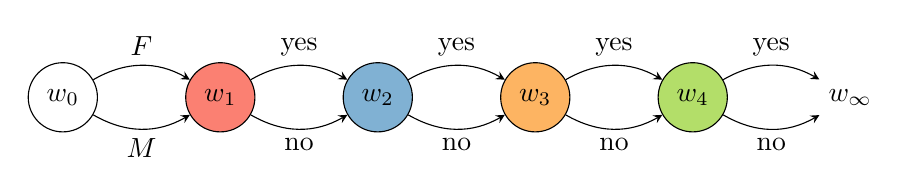
\begin{tikzpicture} [node distance = 2cm, on grid]
\node (v0) [state] {$w_0$};
\node (v1) [state, right = of v0, fill = col4] {$w_1$};
\node (v2) [state, right = of v1, fill = col5] {$w_2$};
\node (v3) [state, right = of v2, fill = col6] {$w_3$};
\node (v4) [state, right = of v3, fill = col7] {$w_4$};
\node (w) [right = of v4] {$w_{\infty}$};
\path [-stealth]
    (v0) edge [bend left] node [above] {$F$} (v1)
    (v0) edge [bend right] node [below] {$M$} (v1)
    (v1) edge [bend left] node [above] {yes} (v2)
    (v1) edge [bend right] node [below] {no} (v2)
    (v2) edge [bend left] node [above] {yes} (v3)
    (v2) edge [bend right] node [below] {no} (v3)
    (v3) edge [bend left] node [above] {yes} (v4)
    (v3) edge [bend right] node [below] {no} (v4)
    (v4) edge [bend left] node [above] {yes} (w)
    (v4) edge [bend right] node [below] {no} (w);
\end{tikzpicture}
}
\caption{$\boldsymbol{X}$-compatible CEG representation for the binary independence model from Example~\ref{exm:independence}}
\label{ceg:indep}
\end{figure}
\begin{example}[Biased Coin]
\label{exm:biascoin}
Another simple hypothesis might be to model the responses to the questionnaires as a series of a possibly biased coin tosses, where the bias depends only on the sex of a respondent. That is, all women have the same probability of responding to every questionnaire and all men have the same probability of responding to every questionnaire. Because the `coin tosses' are assumed to be independent, all florets corresponding to the sub-tree of the event tree rooted at position corresponding to a single sex are in the same stage. The corresponding CEG in Figure \ref{ceg:biascoin} is an $\boldsymbol{X}$-compatible representation of the biased coin flip model.
\end{example}
\begin{figure}
\centering
\scalebox{0.9}{
\begin{tikzpicture} [node distance = 2cm, on grid, auto, scale=0.7]
\node (v0) [state] {$v_0$};
\node (v1F) [state, above right = of v0, fill = col8] {$f_1$};
\node (v2F) [state, right = of v1F, fill = col8] {$f_2$};
\node (v3F) [state, right = of v2F, fill = col8] {$f_3$};
\node (v4F) [state, right = of v3F, fill = col8] {$f_4$}; `  
\node (v1M) [state, below right = of v0, fill = col5] {$m_1$};
\node (v2M) [state, right = of v1M, fill = col5] {$m_2$};
\node (v3M) [state, right = of v2M, fill = col5] {$m_3$};
\node (v4M) [state, right = of v3M, fill = col5] {$m_4$};
\node (w) [right = of v4] {$w_{\infty}$};
\path [-stealth]
    (v0) edge [bend left] node [above] {$F$} (v1F)
    (v1F) edge [bend left] node [above] {yes} (v2F)
    (v1F) edge [bend right] node [below] {no} (v2F)
    (v2F) edge [bend left] node [above] {yes} (v3F)
    (v2F) edge [bend right] node [below] {no} (v3F)
    (v3F) edge [bend left] node [above] {yes} (v4F)
    (v3F) edge [bend right] node [below] {no} (v4F)
    (v4F) edge [bend left] node [above] {yes} (w)
    (v4F) edge [right] node [below] {no} (w)
    (v0) edge [bend right] node [below] {$M$} (v1M)
    (v1M) edge [bend left] node [above] {yes} (v2M)
    (v1M) edge [bend right] node [below] {no} (v2M)
    (v2M) edge [bend left] node [above] {yes} (v3M)
    (v2M) edge [bend right] node [below] {no} (v3M)
    (v3M) edge [bend left] node [above] {yes} (v4M)
    (v3M) edge [bend right] node [below] {no} (v4M)
    (v4M) edge [left] node [above] {yes} (w)
    (v4M) edge [bend right] node [below] {no} (w);
\end{tikzpicture}
}
\caption{$\boldsymbol{X}$-compatible CEG representation for the biased coin-flip model from Example~\ref{exm:biascoin}}
\label{ceg:biascoin}
\end{figure}
\begin{example}[Counting Responses]
\label{exm:counting-responses}
In this example for simplicity we exclude $X_0$ (sex) from the model and instead draw our attention to the number of currently missing responses to the survey. Thus, let $\boldsymbol{X} = (X_1, X_2, X_3, X_4)$. The hypothesis of this example is as follows: Given the wave of the survey, the response to the next questionnaire depends only on the number of already recorded responses. 
If we label the edges of the $\boldsymbol{X}$-compatible staged tree with 1 and 0 to indicate the presence of a response in every survey, then the vertices of the staged tree are in the same stage if and only if they are on the same level of the tree and the sum from the edges of their root-to-vertex paths is equal. Fig~\ref{ceg:counting-responses} represents the CEG for this hypothesis.
\end{example}
\begin{figure}
\centering
\scalebox{0.9}{
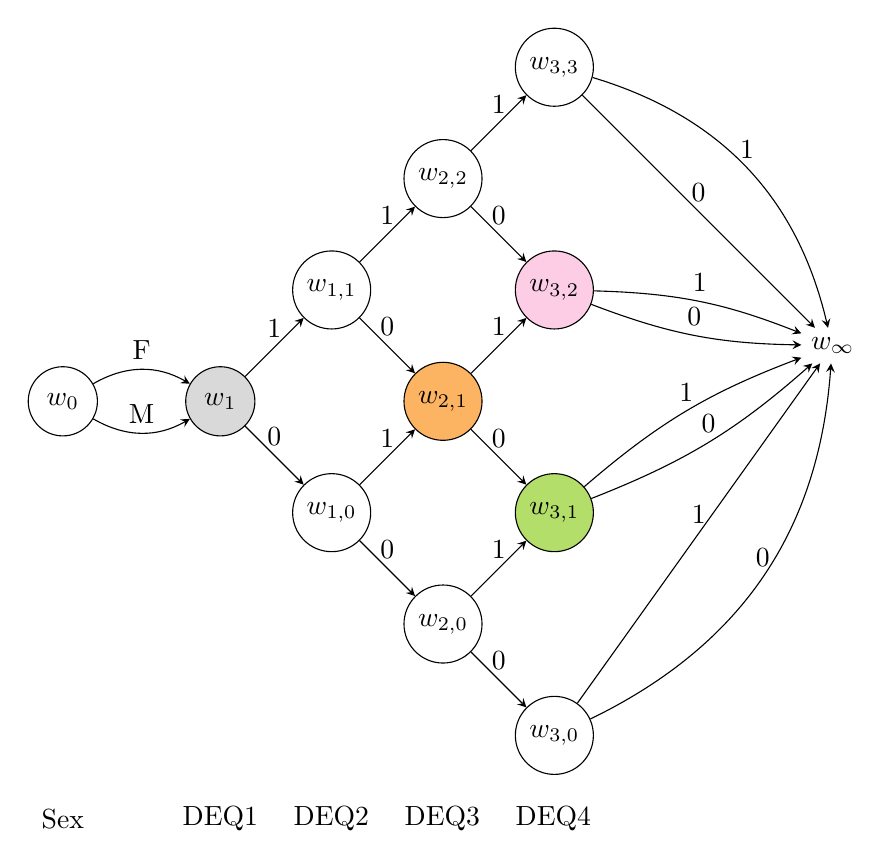
\begin{tikzpicture} [node distance = 2cm, on grid, auto]
\node (v0) [state] {$w_0$};
\node (v1) [state, right = of v0, fill = col9] {$w_1$};
\node (v10) [state, below right = of v1] {$w_{1,0}$};
\node (v11) [state, above right = of v1] {$w_{1,1}$};
\node (v20) [state, below right = of v10] {$w_{2,0}$};
\node (v21) [state, above right = of v10, fill = col6] {$w_{2,1}$};
\node (v22) [state, above right = of v11] {$w_{2,2}$};
\node (v30) [state, below right = of v20] {$w_{3,0}$};
\node (v31) [state, above right = of v20, fill = col7] {$w_{3,1}$};
\node (v32) [state, below right = of v22, fill = col8] {$w_{3,2}$};
\node (v33) [state, above right = of v22] {$w_{3,3}$};
\node (w) [below right = 5cm of v33] {$w_{\infty}$};
\draw  (0,-5.3) node(x0) {Sex};
\draw  (2,-5.3) node(x1) {DEQ1};
\draw  (3.41,-5.3) node(x2) {DEQ2};
\draw  (4.82,-5.3) node(x3) {DEQ3};
\draw  (6.23,-5.3) node(x4) {DEQ4};
\path [-stealth]
    (v0) edge [bend left] node [above] {F} (v1)
    (v0) edge [bend  right] node [above] {M} (v1)
    (v1) edge [left] node [above] {1} (v11)
    (v1) edge [left] node [above] {0} (v10)
    (v10) edge [left] node [above] {0} (v20)
    (v10) edge [left] node [above] {1} (v21)
    (v11) edge [left] node [above] {0} (v21)
    (v11) edge [left] node [above] {1} (v22)
    (v20) edge [left] node [above] {0} (v30)
    (v20) edge [left] node [above] {1} (v31)
    (v21) edge [left] node [above] {0} (v31)
    (v21) edge [left] node [above] {1} (v32)
    (v22) edge [left] node [above] {0} (v32)
    (v22) edge [left] node [above] {1} (v33)
    (v30) edge [bend right] node [above] {0} (w)
    (v30) edge [left] node [above] {1} (w)
    (v31) edge[bend left=10,auto=right] node [above] {1} (w)
    (v31) edge[bend right=10,auto=right] node [above] {0} (w)
    (v32) edge [bend left=10,auto=right] node [above] {1} (w)
    (v32) edge [bend right=10,auto=right] node [above] {0} (w)
    (v33) edge [right] node [above] {0} (w)
    (v33) edge [bend left] node [above] {1} (w);
\end{tikzpicture}
}
\vspace{1ex}
\caption{$\boldsymbol{X}$-compatible CEG representation for the  model from Example~\ref{exm:counting-responses}}
\label{ceg:counting-responses}
\end{figure}

\subsection{Best-scoring CEG of the non-reponse}\label{subsec:best-fit-dropout}
In the previous section we presented several examples on how a modeller might approach the problem of missing responses and how these hypothesis might be expressed with a CEG. If these models were the only competing models we could use a scoring criterion such as the AIC or the Bayes Factor as described in \cite{smith2017cegs} for a bayesian approach in model selection, to choose the best model out of the three. However, from Table~\ref{tab:respondents-sex} we should not expect any of the three examples presented to be an adequate representation of the problem. We therefore introduce another model which was found using the AHC algorithm presented in Fig~\ref{ceg:ahc-responses}. Clearly the structure of this graph is less easy to interpret at first sight. However, the graph illustrates several asymmetries which allow us to draw a number of conclusions that are not obtainable from a regular BN.
\begin{enumerate}[topsep=0pt]
    \item The probability of response to the first survey is dependent on sex. The probability of response to the second survey is dependent on both the sex and the response to the previous survey.
    \item Given that the pattern of responses to the first and second survey is $\{1, 0\}$, i.e. $X_1 = 0$ and $X_2 = 1$, the probability of responding to DEQ3 and DEQ4 is independent of sex. (The paths following edges $\{F, 0, 1\}$, $\{M, 0, 1\}$ are incident on position $w_{12}$).
    \item Given that the pattern of responses to the first and second survey is $\{0, 1\}$, i.e. $X_1 = 1$ and $X_2 = 0$, the probability of responding to DEQ3 is the same for men and women (positions $w_{13}$ and $w_{9}$ are in the same stage), but the probability of responding to DEQ4 differs for men and women ($w_{13}$ and $w_{9}$ are in the same stage, but not merged into one node).
\end{enumerate}
\begin{figure}
\centering

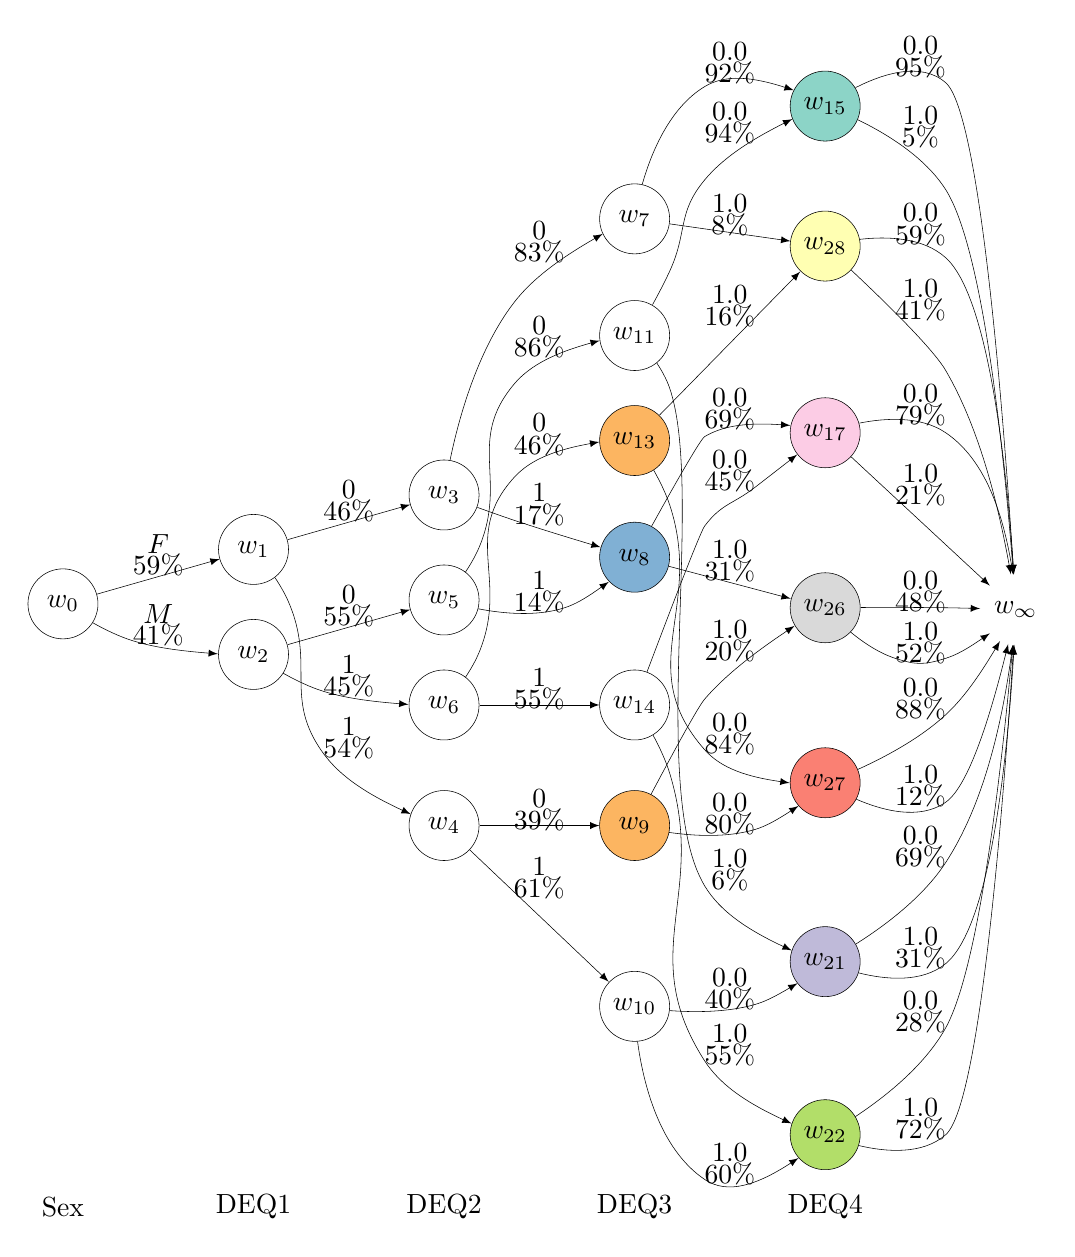
\begin{tikzpicture}[>=latex,line join=bevel, scale = 0.7]
  \pgfsetlinewidth{0.2bp}
%%
\pgfsetcolor{black}
  % Edge: w_{0} -> w_{1}
  \draw [->] (35.52bp,305.22bp) .. controls (50.292bp,309.45bp) and (71.684bp,315.56bp)  .. (98.631bp,323.26bp);
  \definecolor{strokecol}{rgb}{0.0,0.0,0.0};
  \pgfsetstrokecolor{strokecol}
  \draw (67.0bp,331.22bp) node {$F$};
  \draw (67.0bp,320.22bp) node {$59\%$};
  % Edge: w_{0} -> w_{2}
  \pgfsetcolor{black}
  \draw [->] (33.222bp,290.57bp) .. controls (39.439bp,287.06bp) and (46.841bp,283.43bp)  .. (54.0bp,281.22bp) .. controls (64.714bp,277.92bp) and (76.899bp,276.14bp)  .. (97.731bp,274.5bp);
  \definecolor{strokecol}{rgb}{0.0,0.0,0.0};
  \pgfsetstrokecolor{strokecol}
  \draw (67.0bp,295.22bp) node {$M$};
  \draw (67.0bp,284.22bp) node {$41\%$};
  % Edge: w_{1} -> w_{3}
  \pgfsetcolor{black}
  \draw [->] (133.52bp,333.22bp) .. controls (148.29bp,337.45bp) and (169.68bp,343.56bp)  .. (196.63bp,351.26bp);
  \definecolor{strokecol}{rgb}{0.0,0.0,0.0};
  \pgfsetstrokecolor{strokecol}
  \draw (165.0bp,359.22bp) node {$0$};
  \draw (165.0bp,348.22bp) node {$46\%$};
  % Edge: w_{1} -> w_{4}
  \pgfsetcolor{black}
  \draw [->] (127.11bp,313.63bp) .. controls (129.66bp,309.76bp) and (132.17bp,305.46bp)  .. (134.0bp,301.22bp) .. controls (148.1bp,268.55bp) and (131.05bp,251.97bp)  .. (152.0bp,223.22bp) .. controls (160.88bp,211.03bp) and (175.11bp,202.12bp)  .. (196.89bp,192.07bp);
  \definecolor{strokecol}{rgb}{0.0,0.0,0.0};
  \pgfsetstrokecolor{strokecol}
  \draw (165.0bp,237.22bp) node {$1$};
  \draw (165.0bp,226.22bp) node {$54\%$};
  % Edge: w_{2} -> w_{5}
  \pgfsetcolor{black}
  \draw [->] (133.52bp,279.22bp) .. controls (148.29bp,283.45bp) and (169.68bp,289.56bp)  .. (196.63bp,297.26bp);
  \definecolor{strokecol}{rgb}{0.0,0.0,0.0};
  \pgfsetstrokecolor{strokecol}
  \draw (165.0bp,305.22bp) node {$0$};
  \draw (165.0bp,294.22bp) node {$55\%$};
  % Edge: w_{2} -> w_{6}
  \pgfsetcolor{black}
  \draw [->] (131.22bp,264.57bp) .. controls (137.44bp,261.06bp) and (144.84bp,257.43bp)  .. (152.0bp,255.22bp) .. controls (162.71bp,251.92bp) and (174.9bp,250.14bp)  .. (195.73bp,248.5bp);
  \definecolor{strokecol}{rgb}{0.0,0.0,0.0};
  \pgfsetstrokecolor{strokecol}
  \draw (165.0bp,269.22bp) node {$1$};
  \draw (165.0bp,258.22bp) node {$45\%$};
  % Edge: w_{3} -> w_{7}
  \pgfsetcolor{black}
  \draw [->] (217.11bp,374.27bp) .. controls (221.49bp,395.43bp) and (231.13bp,430.74bp)  .. (250.0bp,455.22bp) .. controls (259.69bp,467.79bp) and (274.09bp,478.09bp)  .. (295.63bp,490.5bp);
  \definecolor{strokecol}{rgb}{0.0,0.0,0.0};
  \pgfsetstrokecolor{strokecol}
  \draw (263.0bp,492.22bp) node {$0$};
  \draw (263.0bp,481.22bp) node {$83\%$};
  % Edge: w_{3} -> w_{8}
  \pgfsetcolor{black}
  \draw [->] (231.15bp,349.83bp) .. controls (237.1bp,347.67bp) and (243.82bp,345.28bp)  .. (250.0bp,343.22bp) .. controls (261.33bp,339.44bp) and (273.92bp,335.53bp)  .. (294.56bp,329.32bp);
  \definecolor{strokecol}{rgb}{0.0,0.0,0.0};
  \pgfsetstrokecolor{strokecol}
  \draw (263.0bp,357.22bp) node {$1$};
  \draw (263.0bp,346.22bp) node {$17\%$};
  % Edge: w_{4} -> w_{9}
  \pgfsetcolor{black}
  \draw [->] (232.43bp,186.22bp) .. controls (246.9bp,186.22bp) and (267.28bp,186.22bp)  .. (293.98bp,186.22bp);
  \definecolor{strokecol}{rgb}{0.0,0.0,0.0};
  \pgfsetstrokecolor{strokecol}
  \draw (263.0bp,200.22bp) node {$0$};
  \draw (263.0bp,189.22bp) node {$39\%$};
  % Edge: w_{4} -> w_{10}
  \pgfsetcolor{black}
  \draw [->] (227.22bp,173.68bp) .. controls (243.66bp,158.08bp) and (271.91bp,131.26bp)  .. (298.68bp,105.86bp);
  \definecolor{strokecol}{rgb}{0.0,0.0,0.0};
  \pgfsetstrokecolor{strokecol}
  \draw (263.0bp,165.22bp) node {$1$};
  \draw (263.0bp,154.22bp) node {$61\%$};
  % Edge: w_{5} -> w_{8}
  \pgfsetcolor{black}
  \draw [->] (231.53bp,297.69bp) .. controls (244.19bp,295.23bp) and (261.53bp,293.54bp)  .. (276.0bp,298.22bp) .. controls (281.1bp,299.87bp) and (286.08bp,302.53bp)  .. (298.78bp,311.59bp);
  \definecolor{strokecol}{rgb}{0.0,0.0,0.0};
  \pgfsetstrokecolor{strokecol}
  \draw (263.0bp,312.22bp) node {$1$};
  \draw (263.0bp,301.22bp) node {$14\%$};
  % Edge: w_{5} -> w_{11}
  \pgfsetcolor{black}
  \draw [->] (224.96bp,316.5bp) .. controls (227.59bp,320.45bp) and (230.16bp,324.86bp)  .. (232.0bp,329.22bp) .. controls (246.85bp,364.39bp) and (225.42bp,384.0bp)  .. (250.0bp,413.22bp) .. controls (258.64bp,423.49bp) and (272.12bp,429.58bp)  .. (294.11bp,435.64bp);
  \definecolor{strokecol}{rgb}{0.0,0.0,0.0};
  \pgfsetstrokecolor{strokecol}
  \draw (263.0bp,443.22bp) node {$0$};
  \draw (263.0bp,432.22bp) node {$86\%$};
  % Edge: w_{6} -> w_{13}
  \pgfsetcolor{black}
  \draw [->] (225.01bp,262.48bp) .. controls (227.63bp,266.44bp) and (230.19bp,270.85bp)  .. (232.0bp,275.22bp) .. controls (247.61bp,312.91bp) and (222.63bp,334.97bp)  .. (250.0bp,365.22bp) .. controls (258.59bp,374.71bp) and (271.78bp,379.52bp)  .. (293.89bp,383.49bp);
  \definecolor{strokecol}{rgb}{0.0,0.0,0.0};
  \pgfsetstrokecolor{strokecol}
  \draw (263.0bp,393.22bp) node {$0$};
  \draw (263.0bp,382.22bp) node {$46\%$};
  % Edge: w_{6} -> w_{14}
  \pgfsetcolor{black}
  \draw [->] (232.43bp,248.22bp) .. controls (246.9bp,248.22bp) and (267.28bp,248.22bp)  .. (293.98bp,248.22bp);
  \definecolor{strokecol}{rgb}{0.0,0.0,0.0};
  \pgfsetstrokecolor{strokecol}
  \draw (263.0bp,262.22bp) node {$1$};
  \draw (263.0bp,251.22bp) node {$55\%$};
  % Edge: w_{7} -> w_{15}
  \pgfsetcolor{black}
  \draw [->] (315.93bp,516.01bp) .. controls (320.56bp,532.28bp) and (330.03bp,555.4bp)  .. (348.0bp,566.22bp) .. controls (358.76bp,572.7bp) and (372.4bp,571.32bp)  .. (393.85bp,564.39bp);
  \definecolor{strokecol}{rgb}{0.0,0.0,0.0};
  \pgfsetstrokecolor{strokecol}
  \draw (361.0bp,584.22bp) node {$0.0$};
  \draw (361.0bp,573.22bp) node {$92\%$};
  % Edge: w_{7} -> w_{28}
  \pgfsetcolor{black}
  \draw [->] (329.97bp,495.65bp) .. controls (344.48bp,493.58bp) and (365.15bp,490.63bp)  .. (392.14bp,486.77bp);
  \definecolor{strokecol}{rgb}{0.0,0.0,0.0};
  \pgfsetstrokecolor{strokecol}
  \draw (361.0bp,506.22bp) node {$1.0$};
  \draw (361.0bp,495.22bp) node {$8\%$};
  % Edge: w_{8} -> w_{17}
  \pgfsetcolor{black}
  \draw [->] (320.69bp,340.05bp) .. controls (330.6bp,357.97bp) and (345.73bp,384.86bp)  .. (348.0bp,386.22bp) .. controls (358.02bp,392.2bp) and (370.67bp,393.48bp)  .. (392.15bp,392.01bp);
  \definecolor{strokecol}{rgb}{0.0,0.0,0.0};
  \pgfsetstrokecolor{strokecol}
  \draw (361.0bp,406.22bp) node {$0.0$};
  \draw (361.0bp,395.22bp) node {$69\%$};
  % Edge: w_{8} -> w_{26}
  \pgfsetcolor{black}
  \draw [->] (329.52bp,319.57bp) .. controls (344.2bp,315.68bp) and (365.42bp,310.05bp)  .. (392.3bp,302.91bp);
  \definecolor{strokecol}{rgb}{0.0,0.0,0.0};
  \pgfsetstrokecolor{strokecol}
  \draw (361.0bp,328.22bp) node {$1.0$};
  \draw (361.0bp,317.22bp) node {$31\%$};
  % Edge: w_{9} -> w_{26}
  \pgfsetcolor{black}
  \draw [->] (320.41bp,202.21bp) .. controls (329.89bp,220.09bp) and (344.43bp,247.1bp)  .. (348.0bp,251.22bp) .. controls (358.82bp,263.7bp) and (373.45bp,274.99bp)  .. (394.27bp,288.93bp);
  \definecolor{strokecol}{rgb}{0.0,0.0,0.0};
  \pgfsetstrokecolor{strokecol}
  \draw (361.0bp,287.22bp) node {$1.0$};
  \draw (361.0bp,276.22bp) node {$20\%$};
  % Edge: w_{9} -> w_{27}
  \pgfsetcolor{black}
  \draw [->] (329.76bp,182.67bp) .. controls (342.38bp,180.86bp) and (359.57bp,179.85bp)  .. (374.0bp,184.22bp) .. controls (378.78bp,185.67bp) and (383.51bp,187.98bp)  .. (396.29bp,196.29bp);
  \definecolor{strokecol}{rgb}{0.0,0.0,0.0};
  \pgfsetstrokecolor{strokecol}
  \draw (361.0bp,198.22bp) node {$0.0$};
  \draw (361.0bp,187.22bp) node {$80\%$};
  % Edge: w_{10} -> w_{21}
  \pgfsetcolor{black}
  \draw [->] (330.01bp,91.042bp) .. controls (342.59bp,90.114bp) and (359.63bp,90.05bp)  .. (374.0bp,94.219bp) .. controls (378.47bp,95.517bp) and (382.95bp,97.527bp)  .. (395.78bp,105.1bp);
  \definecolor{strokecol}{rgb}{0.0,0.0,0.0};
  \pgfsetstrokecolor{strokecol}
  \draw (361.0bp,108.22bp) node {$0.0$};
  \draw (361.0bp,97.22bp) node {$40\%$};
  % Edge: w_{10} -> w_{22}
  \pgfsetcolor{black}
  \draw [->] (313.5bp,75.198bp) .. controls (316.34bp,54.109bp) and (324.51bp,20.059bp)  .. (348.0bp,4.219bp) .. controls (360.1bp,-3.9409bp) and (375.48bp,1.6774bp)  .. (396.31bp,15.23bp);
  \definecolor{strokecol}{rgb}{0.0,0.0,0.0};
  \pgfsetstrokecolor{strokecol}
  \draw (361.0bp,18.22bp) node {$1.0$};
  \draw (361.0bp,7.22bp) node {$60\%$};
  % Edge: w_{11} -> w_{15}
  \pgfsetcolor{black}
  \draw [->] (321.23bp,454.11bp) .. controls (324.19bp,459.47bp) and (327.37bp,465.53bp)  .. (330.0bp,471.22bp) .. controls (339.38bp,491.53bp) and (333.7bp,501.02bp)  .. (348.0bp,518.22bp) .. controls (357.55bp,529.71bp) and (371.52bp,538.7bp)  .. (393.14bp,549.56bp);
  \definecolor{strokecol}{rgb}{0.0,0.0,0.0};
  \pgfsetstrokecolor{strokecol}
  \draw (361.0bp,553.22bp) node {$0.0$};
  \draw (361.0bp,542.22bp) node {$94\%$};
  % Edge: w_{11} -> w_{21}
  \pgfsetcolor{black}
  \draw [->] (323.39bp,424.1bp) .. controls (326.01bp,420.14bp) and (328.47bp,415.7bp)  .. (330.0bp,411.22bp) .. controls (348.43bp,357.25bp) and (318.69bp,204.14bp)  .. (348.0bp,155.22bp) .. controls (355.97bp,141.92bp) and (370.41bp,132.44bp)  .. (392.82bp,121.97bp);
  \definecolor{strokecol}{rgb}{0.0,0.0,0.0};
  \pgfsetstrokecolor{strokecol}
  \draw (361.0bp,169.22bp) node {$1.0$};
  \draw (361.0bp,158.22bp) node {$6\%$};
  % Edge: w_{13} -> w_{28}
  \pgfsetcolor{black}
  \draw [->] (324.81bp,397.29bp) .. controls (341.39bp,414.21bp) and (370.46bp,443.88bp)  .. (397.19bp,471.14bp);
  \definecolor{strokecol}{rgb}{0.0,0.0,0.0};
  \pgfsetstrokecolor{strokecol}
  \draw (361.0bp,459.22bp) node {$1.0$};
  \draw (361.0bp,448.22bp) node {$16\%$};
  % Edge: w_{13} -> w_{27}
  \pgfsetcolor{black}
  \draw [->] (321.8bp,368.96bp) .. controls (324.87bp,363.55bp) and (327.98bp,357.29bp)  .. (330.0bp,351.22bp) .. controls (347.83bp,297.53bp) and (310.59bp,267.65bp)  .. (348.0bp,225.22bp) .. controls (356.39bp,215.7bp) and (369.56bp,211.28bp)  .. (391.75bp,208.15bp);
  \definecolor{strokecol}{rgb}{0.0,0.0,0.0};
  \pgfsetstrokecolor{strokecol}
  \draw (361.0bp,239.22bp) node {$0.0$};
  \draw (361.0bp,228.22bp) node {$84\%$};
  % Edge: w_{14} -> w_{17}
  \pgfsetcolor{black}
  \draw [->] (318.38bp,265.21bp) .. controls (328.07bp,290.92bp) and (345.63bp,337.06bp)  .. (348.0bp,340.22bp) .. controls (356.75bp,351.88bp) and (362.47bp,351.3bp)  .. (374.0bp,360.22bp) .. controls (378.35bp,363.58bp) and (382.99bp,367.19bp)  .. (395.65bp,377.03bp);
  \definecolor{strokecol}{rgb}{0.0,0.0,0.0};
  \pgfsetstrokecolor{strokecol}
  \draw (361.0bp,374.22bp) node {$0.0$};
  \draw (361.0bp,363.22bp) node {$45\%$};
  % Edge: w_{14} -> w_{22}
  \pgfsetcolor{black}
  \draw [->] (321.48bp,232.69bp) .. controls (324.68bp,226.79bp) and (327.95bp,219.88bp)  .. (330.0bp,213.22bp) .. controls (349.46bp,149.88bp) and (312.19bp,120.97bp)  .. (348.0bp,65.219bp) .. controls (356.26bp,52.353bp) and (370.59bp,43.155bp)  .. (392.75bp,32.944bp);
  \definecolor{strokecol}{rgb}{0.0,0.0,0.0};
  \pgfsetstrokecolor{strokecol}
  \draw (361.0bp,79.22bp) node {$1.0$};
  \draw (361.0bp,68.22bp) node {$55\%$};
  % Edge: w_{15} -> w_inf
  \pgfsetcolor{black}
  \draw [->] (425.64bp,565.71bp) .. controls (439.44bp,572.74bp) and (459.3bp,579.34bp)  .. (472.0bp,568.22bp) .. controls (490.09bp,552.37bp) and (502.11bp,391.7bp)  .. (506.95bp,315.36bp);
  \definecolor{strokecol}{rgb}{0.0,0.0,0.0};
  \pgfsetstrokecolor{strokecol}
  \draw (459.0bp,587.22bp) node {$0.0$};
  \draw (459.0bp,576.22bp) node {$95\%$};
  % Edge: w_{15} -> w_inf
  \pgfsetcolor{black}
  \draw [->] (426.82bp,549.16bp) .. controls (441.22bp,542.2bp) and (461.27bp,530.15bp)  .. (472.0bp,513.22bp) .. controls (491.52bp,482.41bp) and (502.0bp,376.47bp)  .. (506.79bp,315.27bp);
  \definecolor{strokecol}{rgb}{0.0,0.0,0.0};
  \pgfsetstrokecolor{strokecol}
  \draw (459.0bp,551.22bp) node {$1.0$};
  \draw (459.0bp,540.22bp) node {$5\%$};
  % Edge: w_{28} -> w_inf
  \pgfsetcolor{black}
  \draw [->] (427.74bp,487.68bp) .. controls (441.52bp,489.28bp) and (460.21bp,488.88bp)  .. (472.0bp,478.22bp) .. controls (494.16bp,458.17bp) and (503.14bp,371.23bp)  .. (507.05bp,315.39bp);
  \definecolor{strokecol}{rgb}{0.0,0.0,0.0};
  \pgfsetstrokecolor{strokecol}
  \draw (459.0bp,501.22bp) node {$0.0$};
  \draw (459.0bp,490.22bp) node {$59\%$};
  % Edge: w_{28} -> w_inf
  \pgfsetcolor{black}
  \draw [->] (423.48bp,471.78bp) .. controls (439.62bp,456.66bp) and (465.31bp,431.72bp)  .. (472.0bp,420.22bp) .. controls (489.41bp,390.3bp) and (498.96bp,351.33bp)  .. (505.49bp,315.41bp);
  \definecolor{strokecol}{rgb}{0.0,0.0,0.0};
  \pgfsetstrokecolor{strokecol}
  \draw (459.0bp,462.22bp) node {$1.0$};
  \draw (459.0bp,451.22bp) node {$41\%$};
  % Edge: w_{17} -> w_inf
  \pgfsetcolor{black}
  \draw [->] (427.58bp,393.17bp) .. controls (440.92bp,395.83bp) and (459.09bp,396.99bp)  .. (472.0bp,388.22bp) .. controls (492.55bp,374.25bp) and (501.37bp,346.53bp)  .. (506.68bp,315.25bp);
  \definecolor{strokecol}{rgb}{0.0,0.0,0.0};
  \pgfsetstrokecolor{strokecol}
  \draw (459.0bp,408.22bp) node {$0.0$};
  \draw (459.0bp,397.22bp) node {$79\%$};
  % Edge: w_{17} -> w_inf
  \pgfsetcolor{black}
  \draw [->] (423.22bp,375.95bp) .. controls (439.66bp,360.68bp) and (467.91bp,334.45bp)  .. (494.68bp,309.59bp);
  \definecolor{strokecol}{rgb}{0.0,0.0,0.0};
  \pgfsetstrokecolor{strokecol}
  \draw (459.0bp,367.22bp) node {$1.0$};
  \draw (459.0bp,356.22bp) node {$21\%$};
  % Edge: w_{26} -> w_inf
  \pgfsetcolor{black}
  \draw [->] (428.18bp,298.35bp) .. controls (440.54bp,298.41bp) and (457.25bp,298.42bp)  .. (472.0bp,298.22bp) .. controls (474.43bp,298.19bp) and (476.94bp,298.14bp)  .. (489.69bp,297.83bp);
  \definecolor{strokecol}{rgb}{0.0,0.0,0.0};
  \pgfsetstrokecolor{strokecol}
  \draw (459.0bp,312.22bp) node {$0.0$};
  \draw (459.0bp,301.22bp) node {$48\%$};
  % Edge: w_{26} -> w_inf
  \pgfsetcolor{black}
  \draw [->] (423.22bp,285.59bp) .. controls (429.58bp,280.37bp) and (437.64bp,274.92bp)  .. (446.0bp,272.22bp) .. controls (457.0bp,268.66bp) and (460.97bp,268.77bp)  .. (472.0bp,272.22bp) .. controls (477.04bp,273.8bp) and (482.0bp,276.36bp)  .. (494.7bp,285.07bp);
  \definecolor{strokecol}{rgb}{0.0,0.0,0.0};
  \pgfsetstrokecolor{strokecol}
  \draw (459.0bp,286.22bp) node {$1.0$};
  \draw (459.0bp,275.22bp) node {$52\%$};
  % Edge: w_{27} -> w_inf
  \pgfsetcolor{black}
  \draw [->] (426.91bp,215.13bp) .. controls (440.22bp,221.15bp) and (458.68bp,230.86bp)  .. (472.0bp,243.22bp) .. controls (480.98bp,251.55bp) and (488.82bp,262.55bp)  .. (499.92bp,281.11bp);
  \definecolor{strokecol}{rgb}{0.0,0.0,0.0};
  \pgfsetstrokecolor{strokecol}
  \draw (459.0bp,257.22bp) node {$0.0$};
  \draw (459.0bp,246.22bp) node {$88\%$};
  % Edge: w_{27} -> w_inf
  \pgfsetcolor{black}
  \draw [->] (425.93bp,199.79bp) .. controls (439.37bp,193.95bp) and (458.52bp,188.77bp)  .. (472.0bp,198.22bp) .. controls (484.03bp,206.65bp) and (495.14bp,243.49bp)  .. (504.13bp,279.58bp);
  \definecolor{strokecol}{rgb}{0.0,0.0,0.0};
  \pgfsetstrokecolor{strokecol}
  \draw (459.0bp,212.22bp) node {$1.0$};
  \draw (459.0bp,201.22bp) node {$12\%$};
  % Edge: w_{21} -> w_inf
  \pgfsetcolor{black}
  \draw [->] (425.84bp,125.31bp) .. controls (439.98bp,134.23bp) and (460.23bp,149.1bp)  .. (472.0bp,167.22bp) .. controls (492.28bp,198.42bp) and (501.25bp,240.98bp)  .. (506.44bp,278.99bp);
  \definecolor{strokecol}{rgb}{0.0,0.0,0.0};
  \pgfsetstrokecolor{strokecol}
  \draw (459.0bp,181.22bp) node {$0.0$};
  \draw (459.0bp,170.22bp) node {$69\%$};
  % Edge: w_{21} -> w_inf
  \pgfsetcolor{black}
  \draw [->] (427.22bp,110.43bp) .. controls (440.89bp,107.02bp) and (459.69bp,105.1bp)  .. (472.0bp,115.22bp) .. controls (495.27bp,134.34bp) and (503.75bp,222.64bp)  .. (507.23bp,279.1bp);
  \definecolor{strokecol}{rgb}{0.0,0.0,0.0};
  \pgfsetstrokecolor{strokecol}
  \draw (459.0bp,129.22bp) node {$1.0$};
  \draw (459.0bp,118.22bp) node {$31\%$};
  % Edge: w_{22} -> w_inf
  \pgfsetcolor{black}
  \draw [->] (425.46bp,36.483bp) .. controls (439.95bp,46.04bp) and (460.99bp,62.328bp)  .. (472.0bp,82.219bp) .. controls (489.54bp,113.91bp) and (500.97bp,218.38bp)  .. (506.52bp,279.06bp);
  \definecolor{strokecol}{rgb}{0.0,0.0,0.0};
  \pgfsetstrokecolor{strokecol}
  \draw (459.0bp,96.22bp) node {$0.0$};
  \draw (459.0bp,85.22bp) node {$28\%$};
  % Edge: w_{22} -> w_inf
  \pgfsetcolor{black}
  \draw [->] (427.39bp,21.616bp) .. controls (441.16bp,18.365bp) and (460.01bp,16.725bp)  .. (472.0bp,27.219bp) .. controls (490.03bp,43.006bp) and (502.08bp,203.09bp)  .. (506.95bp,279.15bp);
  \definecolor{strokecol}{rgb}{0.0,0.0,0.0};
  \pgfsetstrokecolor{strokecol}
  \draw (459.0bp,41.22bp) node {$1.0$};
  \draw (459.0bp,30.22bp) node {$72\%$};
  % Node: w_{0}
\begin{scope}
  \definecolor{strokecol}{rgb}{0.0,0.0,0.0};
  \pgfsetstrokecolor{strokecol}
  \definecolor{fillcol}{rgb}{1.0,1.0,1.0};
  \pgfsetfillcolor{fillcol}
  \filldraw [opacity=1] (18.0bp,300.22bp) ellipse (18.0bp and 18.0bp);
  \draw (18.0bp,300.22bp) node {$w_{0}$};
\end{scope}
  % Node: w_{1}
\begin{scope}
  \definecolor{strokecol}{rgb}{0.0,0.0,0.0};
  \pgfsetstrokecolor{strokecol}
  \definecolor{fillcol}{rgb}{1.0,1.0,1.0};
  \pgfsetfillcolor{fillcol}
  \filldraw [opacity=1] (116.0bp,328.22bp) ellipse (18.0bp and 18.0bp);
  \draw (116.0bp,328.22bp) node {$w_{1}$};
\end{scope}
  % Node: w_{2}
\begin{scope}
  \definecolor{strokecol}{rgb}{0.0,0.0,0.0};
  \pgfsetstrokecolor{strokecol}
  \definecolor{fillcol}{rgb}{1.0,1.0,1.0};
  \pgfsetfillcolor{fillcol}
  \filldraw [opacity=1] (116.0bp,274.22bp) ellipse (18.0bp and 18.0bp);
  \draw (116.0bp,274.22bp) node {$w_{2}$};
\end{scope}
  % Node: w_{3}
\begin{scope}
  \definecolor{strokecol}{rgb}{0.0,0.0,0.0};
  \pgfsetstrokecolor{strokecol}
  \definecolor{fillcol}{rgb}{1.0,1.0,1.0};
  \pgfsetfillcolor{fillcol}
  \filldraw [opacity=1] (214.0bp,356.22bp) ellipse (18.0bp and 18.0bp);
  \draw (214.0bp,356.22bp) node {$w_{3}$};
\end{scope}
  % Node: w_{4}
\begin{scope}
  \definecolor{strokecol}{rgb}{0.0,0.0,0.0};
  \pgfsetstrokecolor{strokecol}
  \definecolor{fillcol}{rgb}{1.0,1.0,1.0};
  \pgfsetfillcolor{fillcol}
  \filldraw [opacity=1] (214.0bp,186.22bp) ellipse (18.0bp and 18.0bp);
  \draw (214.0bp,186.22bp) node {$w_{4}$};
\end{scope}
  % Node: w_{5}
\begin{scope}
  \definecolor{strokecol}{rgb}{0.0,0.0,0.0};
  \pgfsetstrokecolor{strokecol}
  \definecolor{fillcol}{rgb}{1.0,1.0,1.0};
  \pgfsetfillcolor{fillcol}
  \filldraw [opacity=1] (214.0bp,302.22bp) ellipse (18.0bp and 18.0bp);
  \draw (214.0bp,302.22bp) node {$w_{5}$};
\end{scope}
  % Node: w_{6}
\begin{scope}
  \definecolor{strokecol}{rgb}{0.0,0.0,0.0};
  \pgfsetstrokecolor{strokecol}
  \definecolor{fillcol}{rgb}{1.0,1.0,1.0};
  \pgfsetfillcolor{fillcol}
  \filldraw [opacity=1] (214.0bp,248.22bp) ellipse (18.0bp and 18.0bp);
  \draw (214.0bp,248.22bp) node {$w_{6}$};
\end{scope}
  % Node: w_{7}
\begin{scope}
  \definecolor{strokecol}{rgb}{0.0,0.0,0.0};
  \pgfsetstrokecolor{strokecol}
  \definecolor{fillcol}{rgb}{1.0,1.0,1.0};
  \pgfsetfillcolor{fillcol}
  \filldraw [opacity=1] (312.0bp,498.22bp) ellipse (18.0bp and 18.0bp);
  \draw (312.0bp,498.22bp) node {$w_{7}$};
\end{scope}
  % Node: w_{8}
\begin{scope}
  \definecolor{strokecol}{rgb}{0.0,0.0,0.0};
  \pgfsetstrokecolor{strokecol}
  \definecolor{fillcol}{rgb}{0.5,0.69,0.83};
  \pgfsetfillcolor{fillcol}
  \filldraw [opacity=1] (312.0bp,324.22bp) ellipse (18.0bp and 18.0bp);
  \draw (312.0bp,324.22bp) node {$w_{8}$};
\end{scope}
  % Node: w_{9}
\begin{scope}
  \definecolor{strokecol}{rgb}{0.0,0.0,0.0};
  \pgfsetstrokecolor{strokecol}
  \definecolor{fillcol}{rgb}{0.99,0.71,0.38};
  \pgfsetfillcolor{fillcol}
  \filldraw [opacity=1] (312.0bp,186.22bp) ellipse (18.0bp and 18.0bp);
  \draw (312.0bp,186.22bp) node {$w_{9}$};
\end{scope}
  % Node: w_{10}
\begin{scope}
  \definecolor{strokecol}{rgb}{0.0,0.0,0.0};
  \pgfsetstrokecolor{strokecol}
  \definecolor{fillcol}{rgb}{1.0,1.0,1.0};
  \pgfsetfillcolor{fillcol}
  \filldraw [opacity=1] (312.0bp,93.22bp) ellipse (18.0bp and 18.0bp);
  \draw (312.0bp,93.219bp) node {$w_{10}$};
\end{scope}
  % Node: w_{11}
\begin{scope}
  \definecolor{strokecol}{rgb}{0.0,0.0,0.0};
  \pgfsetstrokecolor{strokecol}
  \definecolor{fillcol}{rgb}{1.0,1.0,1.0};
  \pgfsetfillcolor{fillcol}
  \filldraw [opacity=1] (312.0bp,438.22bp) ellipse (18.0bp and 18.0bp);
  \draw (312.0bp,438.22bp) node {$w_{11}$};
\end{scope}
  % Node: w_{13}
\begin{scope}
  \definecolor{strokecol}{rgb}{0.0,0.0,0.0};
  \pgfsetstrokecolor{strokecol}
  \definecolor{fillcol}{rgb}{0.99,0.71,0.38};
  \pgfsetfillcolor{fillcol}
  \filldraw [opacity=1] (312.0bp,384.22bp) ellipse (18.0bp and 18.0bp);
  \draw (312.0bp,384.22bp) node {$w_{13}$};
\end{scope}
  % Node: w_{14}
\begin{scope}
  \definecolor{strokecol}{rgb}{0.0,0.0,0.0};
  \pgfsetstrokecolor{strokecol}
  \definecolor{fillcol}{rgb}{1.0,1.0,1.0};
  \pgfsetfillcolor{fillcol}
  \filldraw [opacity=1] (312.0bp,248.22bp) ellipse (18.0bp and 18.0bp);
  \draw (312.0bp,248.22bp) node {$w_{14}$};
\end{scope}
  % Node: w_{15}
\begin{scope}
  \definecolor{strokecol}{rgb}{0.0,0.0,0.0};
  \pgfsetstrokecolor{strokecol}
  \definecolor{fillcol}{rgb}{0.55,0.83,0.78};
  \pgfsetfillcolor{fillcol}
  \filldraw [opacity=1] (410.0bp,556.22bp) ellipse (18.0bp and 18.0bp);
  \draw (410.0bp,556.22bp) node {$w_{15}$};
\end{scope}
  % Node: w_{28}
\begin{scope}
  \definecolor{strokecol}{rgb}{0.0,0.0,0.0};
  \pgfsetstrokecolor{strokecol}
  \definecolor{fillcol}{rgb}{1.0,1.0,0.7};
  \pgfsetfillcolor{fillcol}
  \filldraw [opacity=1] (410.0bp,484.22bp) ellipse (18.0bp and 18.0bp);
  \draw (410.0bp,484.22bp) node {$w_{28}$};
\end{scope}
  % Node: w_{17}
\begin{scope}
  \definecolor{strokecol}{rgb}{0.0,0.0,0.0};
  \pgfsetstrokecolor{strokecol}
  \definecolor{fillcol}{rgb}{0.99,0.8,0.9};
  \pgfsetfillcolor{fillcol}
  \filldraw [opacity=1] (410.0bp,388.22bp) ellipse (18.0bp and 18.0bp);
  \draw (410.0bp,388.22bp) node {$w_{17}$};
\end{scope}
  % Node: w_{26}
\begin{scope}
  \definecolor{strokecol}{rgb}{0.0,0.0,0.0};
  \pgfsetstrokecolor{strokecol}
  \definecolor{fillcol}{rgb}{0.85,0.85,0.85};
  \pgfsetfillcolor{fillcol}
  \filldraw [opacity=1] (410.0bp,298.22bp) ellipse (18.0bp and 18.0bp);
  \draw (410.0bp,298.22bp) node {$w_{26}$};
\end{scope}
  % Node: w_{27}
\begin{scope}
  \definecolor{strokecol}{rgb}{0.0,0.0,0.0};
  \pgfsetstrokecolor{strokecol}
  \definecolor{fillcol}{rgb}{0.98,0.5,0.45};
  \pgfsetfillcolor{fillcol}
  \filldraw [opacity=1] (410.0bp,208.22bp) ellipse (18.0bp and 18.0bp);
  \draw (410.0bp,208.22bp) node {$w_{27}$};
\end{scope}
  % Node: w_{21}
\begin{scope}
  \definecolor{strokecol}{rgb}{0.0,0.0,0.0};
  \pgfsetstrokecolor{strokecol}
  \definecolor{fillcol}{rgb}{0.75,0.73,0.85};
  \pgfsetfillcolor{fillcol}
  \filldraw [opacity=1] (410.0bp,116.22bp) ellipse (18.0bp and 18.0bp);
  \draw (410.0bp,116.22bp) node {$w_{21}$};
\end{scope}
  % Node: w_{22}
\begin{scope}
  \definecolor{strokecol}{rgb}{0.0,0.0,0.0};
  \pgfsetstrokecolor{strokecol}
  \definecolor{fillcol}{rgb}{0.7,0.87,0.41};
  \pgfsetfillcolor{fillcol}
  \filldraw [opacity=1] (410.0bp,27.22bp) ellipse (18.0bp and 18.0bp);
  \draw (410.0bp,27.219bp) node {$w_{22}$};
\end{scope}
  % Node: w_inf
\begin{scope}
  \definecolor{strokecol}{rgb}{0.0,0.0,0.0};
  \pgfsetstrokecolor{strokecol}
  \draw (508.0bp,297.22bp) node {$w_\infty$};
\end{scope}
%
\begin{scope}
  \draw (18.0bp, -10bp) node {Sex};
  \draw (116.0bp, -10bp) node {DEQ1};
  \draw (214.0bp, -10bp) node {DEQ2};
  \draw (312.0bp, -10bp) node {DEQ3};
  \draw (410.0bp, -10bp) node {DEQ4};
\end{scope}
\end{tikzpicture}


\vspace{1ex}
\caption{The highest scoring CEG found by the AHC algorithm together with the transition probabilities (colours applied only to stages for which more than one situation of the underlying staged tree shares the same floret parameter vector $\boldsymbol{\theta}$)}
\label{ceg:ahc-responses}
\end{figure}
By following the root to sink paths we can observe how the probability of responding to the next survey increases when the response to the previous survey was also recorded. However, due to the complexity of this graph it is not as easy to examine when presented in its full form. We therefore suggest a more compact representation by introducing a new variable $X_{1,2}$. taking values ${00, 01, 10, 11}$ which indicates the responses to the first two ways of the survey. The new CEG on $\boldsymbol{X} = (X_0, X_{1,2}, X_3, X_4)$ is presented on Fig~\ref{ceg:compact-responses}
\begin{figure}
\centering
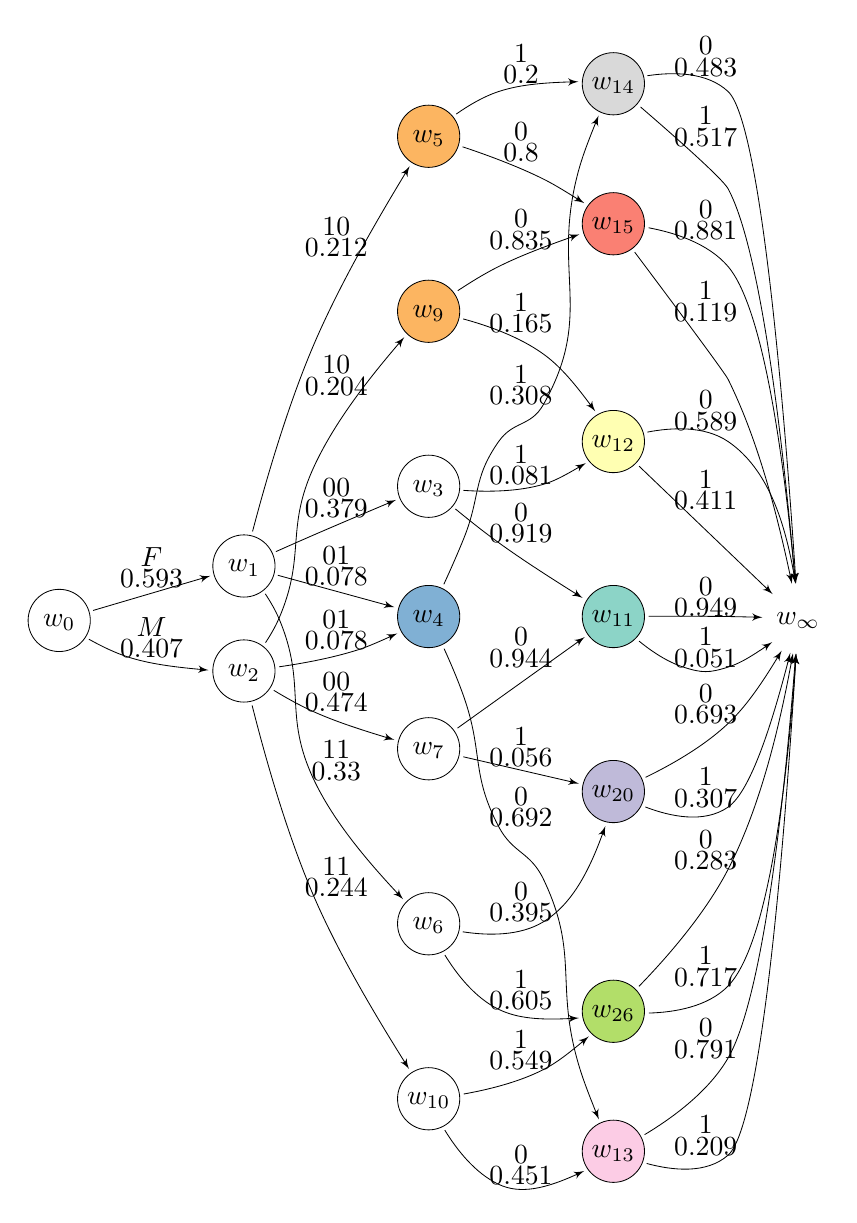
\begin{tikzpicture}[anchor=mid,>=latex',line join=bevel, scale = 0.7]
  \pgfsetlinewidth{0.3bp}
%%
\pgfsetcolor{black}
  % Edge: w_{0} -> w_{1}
  \draw [->] (35.424bp,298.34bp) .. controls (49.485bp,302.49bp) and (69.52bp,308.39bp)  .. (95.686bp,316.1bp);
  \definecolor{strokecol}{rgb}{0.0,0.0,0.0};
  \pgfsetstrokecolor{strokecol}
  \draw (65.5bp,324.21bp) node {$F$};
  \draw (65.5bp,313.21bp) node {$0.593$};
  % Edge: w_{0} -> w_{2}
  \pgfsetcolor{black}
  \draw [->] (33.228bp,283.58bp) .. controls (39.446bp,280.07bp) and (46.848bp,276.43bp)  .. (54.0bp,274.21bp) .. controls (63.764bp,271.17bp) and (74.814bp,269.43bp)  .. (94.828bp,267.65bp);
  \definecolor{strokecol}{rgb}{0.0,0.0,0.0};
  \pgfsetstrokecolor{strokecol}
  \draw (65.5bp,288.21bp) node {$M$};
  \draw (65.5bp,277.21bp) node {$0.407$};
  % Edge: w_{1} -> w_{3}
  \pgfsetcolor{black}
  \draw [->] (129.46bp,328.6bp) .. controls (135.59bp,331.33bp) and (142.6bp,334.43bp)  .. (149.0bp,337.21bp) .. controls (159.75bp,341.87bp) and (171.64bp,346.93bp)  .. (191.18bp,355.17bp);
  \definecolor{strokecol}{rgb}{0.0,0.0,0.0};
  \pgfsetstrokecolor{strokecol}
  \draw (160.5bp,360.21bp) node {$00$};
  \draw (160.5bp,349.21bp) node {$0.379$};
  % Edge: w_{1} -> w_{4}
  \pgfsetcolor{black}
  \draw [->] (130.42bp,316.44bp) .. controls (144.4bp,312.61bp) and (164.27bp,307.18bp)  .. (190.36bp,300.03bp);
  \definecolor{strokecol}{rgb}{0.0,0.0,0.0};
  \pgfsetstrokecolor{strokecol}
  \draw (160.5bp,325.21bp) node {$01$};
  \draw (160.5bp,314.21bp) node {$0.078$};
  % Edge: w_{1} -> w_{5}
  \pgfsetcolor{black}
  \draw [->] (117.44bp,338.98bp) .. controls (123.39bp,361.75bp) and (134.86bp,402.2bp)  .. (149.0bp,435.21bp) .. controls (161.67bp,464.76bp) and (180.02bp,496.83bp)  .. (198.19bp,526.75bp);
  \definecolor{strokecol}{rgb}{0.0,0.0,0.0};
  \pgfsetstrokecolor{strokecol}
  \draw (160.5bp,494.21bp) node {$10$};
  \draw (160.5bp,483.21bp) node {$0.212$};
  % Edge: w_{1} -> w_{6}
  \pgfsetcolor{black}
  \draw [->] (123.96bp,306.92bp) .. controls (126.58bp,302.97bp) and (129.15bp,298.56bp)  .. (131.0bp,294.21bp) .. controls (145.73bp,259.45bp) and (132.81bp,245.3bp)  .. (149.0bp,211.21bp) .. controls (158.6bp,190.98bp) and (174.7bp,171.32bp)  .. (194.85bp,149.83bp);
  \definecolor{strokecol}{rgb}{0.0,0.0,0.0};
  \pgfsetstrokecolor{strokecol}
  \draw (160.5bp,225.21bp) node {$11$};
  \draw (160.5bp,214.21bp) node {$0.33$};
  % Edge: w_{2} -> w_{4}
  \pgfsetcolor{black}
  \draw [->] (131.11bp,269.36bp) .. controls (142.94bp,271.06bp) and (158.62bp,273.88bp)  .. (172.0bp,278.21bp) .. controls (175.46bp,279.33bp) and (179.02bp,280.7bp)  .. (191.87bp,286.51bp);
  \definecolor{strokecol}{rgb}{0.0,0.0,0.0};
  \pgfsetstrokecolor{strokecol}
  \draw (160.5bp,292.21bp) node {$01$};
  \draw (160.5bp,281.21bp) node {$0.078$};
  % Edge: w_{2} -> w_{7}
  \pgfsetcolor{black}
  \draw [->] (128.38bp,257.25bp) .. controls (134.62bp,253.47bp) and (142.0bp,249.33bp)  .. (149.0bp,246.21bp) .. controls (159.1bp,241.7bp) and (170.59bp,237.75bp)  .. (190.33bp,231.81bp);
  \definecolor{strokecol}{rgb}{0.0,0.0,0.0};
  \pgfsetstrokecolor{strokecol}
  \draw (160.5bp,260.21bp) node {$00$};
  \draw (160.5bp,249.21bp) node {$0.474$};
  % Edge: w_{2} -> w_{9}
  \pgfsetcolor{black}
  \draw [->] (124.11bp,281.79bp) .. controls (126.66bp,285.67bp) and (129.17bp,289.97bp)  .. (131.0bp,294.21bp) .. controls (145.1bp,326.87bp) and (134.13bp,339.89bp)  .. (149.0bp,372.21bp) .. controls (159.04bp,394.03bp) and (175.61bp,415.78bp)  .. (195.45bp,438.87bp);
  \definecolor{strokecol}{rgb}{0.0,0.0,0.0};
  \pgfsetstrokecolor{strokecol}
  \draw (160.5bp,423.21bp) node {$10$};
  \draw (160.5bp,412.21bp) node {$0.204$};
  % Edge: w_{2} -> w_{10}
  \pgfsetcolor{black}
  \draw [->] (117.23bp,249.49bp) .. controls (123.03bp,226.37bp) and (134.43bp,184.88bp)  .. (149.0bp,151.21bp) .. controls (161.37bp,122.63bp) and (179.5bp,91.827bp)  .. (197.91bp,62.522bp);
  \definecolor{strokecol}{rgb}{0.0,0.0,0.0};
  \pgfsetstrokecolor{strokecol}
  \draw (160.5bp,165.21bp) node {$11$};
  \draw (160.5bp,154.21bp) node {$0.244$};
  % Edge: w_{3} -> w_{11}
  \pgfsetcolor{black}
  \draw [->] (221.75bp,350.56bp) .. controls (228.35bp,345.12bp) and (236.45bp,338.66bp)  .. (244.0bp,333.21bp) .. controls (255.11bp,325.19bp) and (267.85bp,316.88bp)  .. (287.17bp,304.77bp);
  \definecolor{strokecol}{rgb}{0.0,0.0,0.0};
  \pgfsetstrokecolor{strokecol}
  \draw (255.5bp,347.21bp) node {$0$};
  \draw (255.5bp,336.21bp) node {$0.919$};
  % Edge: w_{3} -> w_{12}
  \pgfsetcolor{black}
  \draw [->] (225.92bp,360.1bp) .. controls (237.81bp,359.28bp) and (253.62bp,359.32bp)  .. (267.0bp,363.21bp) .. controls (271.47bp,364.51bp) and (275.95bp,366.52bp)  .. (288.78bp,374.1bp);
  \definecolor{strokecol}{rgb}{0.0,0.0,0.0};
  \pgfsetstrokecolor{strokecol}
  \draw (255.5bp,377.21bp) node {$1$};
  \draw (255.5bp,366.21bp) node {$0.081$};
  % Edge: w_{4} -> w_{13}
  \pgfsetcolor{black}
  \draw [->] (215.94bp,278.68bp) .. controls (219.31bp,271.3bp) and (223.11bp,262.42bp)  .. (226.0bp,254.21bp) .. controls (236.23bp,225.12bp) and (229.65bp,214.5bp)  .. (244.0bp,187.21bp) .. controls (251.34bp,173.25bp) and (260.19bp,174.43bp)  .. (267.0bp,160.21bp) .. controls (285.55bp,121.45bp) and (272.96bp,106.46bp)  .. (285.0bp,65.207bp) .. controls (286.86bp,58.846bp) and (289.27bp,52.14bp)  .. (295.55bp,36.607bp);
  \definecolor{strokecol}{rgb}{0.0,0.0,0.0};
  \pgfsetstrokecolor{strokecol}
  \draw (255.5bp,201.21bp) node {$0$};
  \draw (255.5bp,190.21bp) node {$0.692$};
  % Edge: w_{4} -> w_{14}
  \pgfsetcolor{black}
  \draw [->] (215.82bp,311.82bp) .. controls (219.1bp,318.96bp) and (222.86bp,327.44bp)  .. (226.0bp,335.21bp) .. controls (234.85bp,357.1bp) and (230.41bp,365.89bp)  .. (244.0bp,385.21bp) .. controls (251.63bp,396.05bp) and (260.47bp,392.67bp)  .. (267.0bp,404.21bp) .. controls (293.54bp,451.15bp) and (270.89bp,472.16bp)  .. (285.0bp,524.21bp) .. controls (286.73bp,530.6bp) and (289.1bp,537.32bp)  .. (295.39bp,552.85bp);
  \definecolor{strokecol}{rgb}{0.0,0.0,0.0};
  \pgfsetstrokecolor{strokecol}
  \draw (255.5bp,418.21bp) node {$1$};
  \draw (255.5bp,407.21bp) node {$0.308$};
  % Edge: w_{5} -> w_{14}
  \pgfsetcolor{black}
  \draw [->] (222.21bp,553.63bp) .. controls (228.51bp,558.05bp) and (236.25bp,562.66bp)  .. (244.0bp,565.21bp) .. controls (253.74bp,568.41bp) and (264.86bp,569.73bp)  .. (285.0bp,570.27bp);
  \definecolor{strokecol}{rgb}{0.0,0.0,0.0};
  \pgfsetstrokecolor{strokecol}
  \draw (255.5bp,583.21bp) node {$1$};
  \draw (255.5bp,572.21bp) node {$0.2$};
  % Edge: w_{5} -> w_{15}
  \pgfsetcolor{black}
  \draw [->] (225.45bp,536.79bp) .. controls (237.41bp,532.81bp) and (253.5bp,526.94bp)  .. (267.0bp,520.21bp) .. controls (271.14bp,518.14bp) and (275.41bp,515.71bp)  .. (288.0bp,507.8bp);
  \definecolor{strokecol}{rgb}{0.0,0.0,0.0};
  \pgfsetstrokecolor{strokecol}
  \draw (255.5bp,543.21bp) node {$0$};
  \draw (255.5bp,532.21bp) node {$0.8$};
  % Edge: w_{6} -> w_{20}
  \pgfsetcolor{black}
  \draw [->] (225.55bp,133.08bp) .. controls (238.02bp,131.15bp) and (254.67bp,130.69bp)  .. (267.0bp,138.21bp) .. controls (281.29bp,146.92bp) and (290.26bp,163.43bp)  .. (298.86bp,187.43bp);
  \definecolor{strokecol}{rgb}{0.0,0.0,0.0};
  \pgfsetstrokecolor{strokecol}
  \draw (255.5bp,152.21bp) node {$0$};
  \draw (255.5bp,141.21bp) node {$0.395$};
  % Edge: w_{6} -> w_{26}
  \pgfsetcolor{black}
  \draw [->] (216.35bp,121.12bp) .. controls (222.51bp,111.11bp) and (231.92bp,99.058bp)  .. (244.0bp,93.207bp) .. controls (253.51bp,88.601bp) and (264.94bp,87.545bp)  .. (285.32bp,88.754bp);
  \definecolor{strokecol}{rgb}{0.0,0.0,0.0};
  \pgfsetstrokecolor{strokecol}
  \draw (255.5bp,107.21bp) node {$1$};
  \draw (255.5bp,96.21bp) node {$0.605$};
  % Edge: w_{7} -> w_{11}
  \pgfsetcolor{black}
  \draw [->] (222.84bp,237.83bp) .. controls (238.18bp,248.81bp) and (262.32bp,266.09bp)  .. (288.26bp,284.66bp);
  \definecolor{strokecol}{rgb}{0.0,0.0,0.0};
  \pgfsetstrokecolor{strokecol}
  \draw (255.5bp,283.21bp) node {$0$};
  \draw (255.5bp,272.21bp) node {$0.944$};
  % Edge: w_{7} -> w_{20}
  \pgfsetcolor{black}
  \draw [->] (225.87bp,223.07bp) .. controls (239.8bp,219.84bp) and (259.4bp,215.3bp)  .. (285.21bp,209.33bp);
  \definecolor{strokecol}{rgb}{0.0,0.0,0.0};
  \pgfsetstrokecolor{strokecol}
  \draw (255.5bp,232.21bp) node {$1$};
  \draw (255.5bp,221.21bp) node {$0.056$};
  % Edge: w_{9} -> w_{12}
  \pgfsetcolor{black}
  \draw [->] (225.73bp,448.28bp) .. controls (238.12bp,444.92bp) and (254.6bp,439.18bp)  .. (267.0bp,430.21bp) .. controls (274.81bp,424.56bp) and (281.83bp,416.79bp)  .. (293.66bp,400.77bp);
  \definecolor{strokecol}{rgb}{0.0,0.0,0.0};
  \pgfsetstrokecolor{strokecol}
  \draw (255.5bp,455.21bp) node {$1$};
  \draw (255.5bp,444.21bp) node {$0.165$};
  % Edge: w_{9} -> w_{15}
  \pgfsetcolor{black}
  \draw [->] (223.0bp,462.8bp) .. controls (229.31bp,466.98bp) and (236.83bp,471.63bp)  .. (244.0bp,475.21bp) .. controls (254.12bp,480.26bp) and (265.71bp,484.82bp)  .. (285.55bp,491.79bp);
  \definecolor{strokecol}{rgb}{0.0,0.0,0.0};
  \pgfsetstrokecolor{strokecol}
  \draw (255.5bp,498.21bp) node {$0$};
  \draw (255.5bp,487.21bp) node {$0.835$};
  % Edge: w_{10} -> w_{13}
  \pgfsetcolor{black}
  \draw [->] (216.32bp,31.056bp) .. controls (222.47bp,21.014bp) and (231.87bp,8.9555bp)  .. (244.0bp,3.2073bp) .. controls (255.03bp,-2.018bp) and (267.99bp,0.82859bp)  .. (287.97bp,10.076bp);
  \definecolor{strokecol}{rgb}{0.0,0.0,0.0};
  \pgfsetstrokecolor{strokecol}
  \draw (255.5bp,17.21bp) node {$0$};
  \draw (255.5bp,6.21bp) node {$0.451$};
  % Edge: w_{10} -> w_{26}
  \pgfsetcolor{black}
  \draw [->] (226.03bp,49.651bp) .. controls (238.11bp,51.793bp) and (254.1bp,55.626bp)  .. (267.0bp,62.207bp) .. controls (272.48bp,65.003bp) and (277.86bp,68.763bp)  .. (290.35bp,79.257bp);
  \definecolor{strokecol}{rgb}{0.0,0.0,0.0};
  \pgfsetstrokecolor{strokecol}
  \draw (255.5bp,76.21bp) node {$1$};
  \draw (255.5bp,65.21bp) node {$0.549$};
  % Edge: w_{11} -> w_inf
  \pgfsetcolor{black}
  \draw [->] (321.08bp,295.34bp) .. controls (332.75bp,295.39bp) and (348.28bp,295.4bp)  .. (362.0bp,295.21bp) .. controls (364.43bp,295.17bp) and (366.94bp,295.13bp)  .. (379.69bp,294.81bp);
  \definecolor{strokecol}{rgb}{0.0,0.0,0.0};
  \pgfsetstrokecolor{strokecol}
  \draw (350.5bp,309.21bp) node {$0$};
  \draw (350.5bp,298.21bp) node {$0.949$};
  % Edge: w_{11} -> w_inf
  \pgfsetcolor{black}
  \draw [->] (316.22bp,282.58bp) .. controls (322.58bp,277.36bp) and (330.64bp,271.91bp)  .. (339.0bp,269.21bp) .. controls (348.73bp,266.06bp) and (352.24bp,266.15bp)  .. (362.0bp,269.21bp) .. controls (367.04bp,270.79bp) and (372.0bp,273.35bp)  .. (384.7bp,282.06bp);
  \definecolor{strokecol}{rgb}{0.0,0.0,0.0};
  \pgfsetstrokecolor{strokecol}
  \draw (350.5bp,283.21bp) node {$1$};
  \draw (350.5bp,272.21bp) node {$0.051$};
  % Edge: w_{12} -> w_inf
  \pgfsetcolor{black}
  \draw [->] (320.52bp,390.07bp) .. controls (333.13bp,392.49bp) and (349.97bp,393.38bp)  .. (362.0bp,385.21bp) .. controls (382.55bp,371.23bp) and (391.37bp,343.52bp)  .. (396.68bp,312.24bp);
  \definecolor{strokecol}{rgb}{0.0,0.0,0.0};
  \pgfsetstrokecolor{strokecol}
  \draw (350.5bp,405.21bp) node {$0$};
  \draw (350.5bp,394.21bp) node {$0.589$};
  % Edge: w_{12} -> w_inf
  \pgfsetcolor{black}
  \draw [->] (316.21bp,372.55bp) .. controls (332.09bp,357.34bp) and (358.92bp,331.64bp)  .. (384.9bp,306.75bp);
  \definecolor{strokecol}{rgb}{0.0,0.0,0.0};
  \pgfsetstrokecolor{strokecol}
  \draw (350.5bp,364.21bp) node {$1$};
  \draw (350.5bp,353.21bp) node {$0.411$};
  % Edge: w_{13} -> w_inf
  \pgfsetcolor{black}
  \draw [->] (319.07bp,28.765bp) .. controls (332.81bp,36.977bp) and (351.91bp,50.704bp)  .. (362.0bp,68.207bp) .. controls (381.17bp,101.46bp) and (391.91bp,213.23bp)  .. (396.78bp,276.11bp);
  \definecolor{strokecol}{rgb}{0.0,0.0,0.0};
  \pgfsetstrokecolor{strokecol}
  \draw (350.5bp,82.21bp) node {$0$};
  \draw (350.5bp,71.21bp) node {$0.791$};
  % Edge: w_{13} -> w_inf
  \pgfsetcolor{black}
  \draw [->] (320.09bp,13.948bp) .. controls (333.15bp,10.373bp) and (350.76bp,8.3345bp)  .. (362.0bp,18.207bp) .. controls (380.45bp,34.403bp) and (392.29bp,198.76bp)  .. (397.0bp,276.15bp);
  \definecolor{strokecol}{rgb}{0.0,0.0,0.0};
  \pgfsetstrokecolor{strokecol}
  \draw (350.5bp,32.21bp) node {$1$};
  \draw (350.5bp,21.21bp) node {$0.209$};
  % Edge: w_{14} -> w_inf
  \pgfsetcolor{black}
  \draw [->] (320.53bp,573.35bp) .. controls (333.65bp,575.32bp) and (351.14bp,575.39bp)  .. (362.0bp,565.21bp) .. controls (379.55bp,548.76bp) and (391.88bp,388.43bp)  .. (396.91bp,312.29bp);
  \definecolor{strokecol}{rgb}{0.0,0.0,0.0};
  \pgfsetstrokecolor{strokecol}
  \draw (350.5bp,587.21bp) node {$0$};
  \draw (350.5bp,576.21bp) node {$0.483$};
  % Edge: w_{14} -> w_inf
  \pgfsetcolor{black}
  \draw [->] (316.97bp,557.28bp) .. controls (333.5bp,543.03bp) and (359.16bp,520.46bp)  .. (362.0bp,515.21bp) .. controls (379.78bp,482.32bp) and (391.16bp,374.12bp)  .. (396.6bp,312.17bp);
  \definecolor{strokecol}{rgb}{0.0,0.0,0.0};
  \pgfsetstrokecolor{strokecol}
  \draw (350.5bp,551.21bp) node {$1$};
  \draw (350.5bp,540.21bp) node {$0.517$};
  % Edge: w_{15} -> w_inf
  \pgfsetcolor{black}
  \draw [->] (321.14bp,495.14bp) .. controls (334.4bp,492.66bp) and (351.8bp,487.2bp)  .. (362.0bp,475.21bp) .. controls (381.32bp,452.51bp) and (391.57bp,367.17bp)  .. (396.62bp,312.29bp);
  \definecolor{strokecol}{rgb}{0.0,0.0,0.0};
  \pgfsetstrokecolor{strokecol}
  \draw (350.5bp,503.21bp) node {$0$};
  \draw (350.5bp,492.21bp) node {$0.881$};
  % Edge: w_{15} -> w_inf
  \pgfsetcolor{black}
  \draw [->] (313.96bp,482.63bp) .. controls (330.53bp,460.54bp) and (360.24bp,420.76bp)  .. (362.0bp,417.21bp) .. controls (377.3bp,386.33bp) and (387.26bp,347.8bp)  .. (394.83bp,312.04bp);
  \definecolor{strokecol}{rgb}{0.0,0.0,0.0};
  \pgfsetstrokecolor{strokecol}
  \draw (350.5bp,461.21bp) node {$1$};
  \draw (350.5bp,450.21bp) node {$0.119$};
  % Edge: w_{20} -> w_inf
  \pgfsetcolor{black}
  \draw [->] (319.59bp,212.54bp) .. controls (332.21bp,218.67bp) and (349.47bp,228.32bp)  .. (362.0bp,240.21bp) .. controls (370.67bp,248.43bp) and (378.34bp,259.12bp)  .. (389.57bp,277.68bp);
  \definecolor{strokecol}{rgb}{0.0,0.0,0.0};
  \pgfsetstrokecolor{strokecol}
  \draw (350.5bp,254.21bp) node {$0$};
  \draw (350.5bp,243.21bp) node {$0.693$};
  % Edge: w_{20} -> w_inf
  \pgfsetcolor{black}
  \draw [->] (319.46bp,197.27bp) .. controls (332.16bp,192.4bp) and (349.61bp,188.59bp)  .. (362.0bp,197.21bp) .. controls (373.73bp,205.37bp) and (384.78bp,240.84bp)  .. (393.98bp,276.5bp);
  \definecolor{strokecol}{rgb}{0.0,0.0,0.0};
  \pgfsetstrokecolor{strokecol}
  \draw (350.5bp,211.21bp) node {$1$};
  \draw (350.5bp,200.21bp) node {$0.307$};
  % Edge: w_{26} -> w_inf
  \pgfsetcolor{black}
  \draw [->] (316.13bp,105.02bp) .. controls (329.49bp,118.74bp) and (349.9bp,141.74bp)  .. (362.0bp,165.21bp) .. controls (378.83bp,197.87bp) and (388.6bp,239.36bp)  .. (395.36bp,276.26bp);
  \definecolor{strokecol}{rgb}{0.0,0.0,0.0};
  \pgfsetstrokecolor{strokecol}
  \draw (350.5bp,179.21bp) node {$0$};
  \draw (350.5bp,168.21bp) node {$0.283$};
  % Edge: w_{26} -> w_inf
  \pgfsetcolor{black}
  \draw [->] (321.23bp,91.283bp) .. controls (334.36bp,91.655bp) and (351.55bp,94.451bp)  .. (362.0bp,105.21bp) .. controls (383.87bp,127.71bp) and (393.03bp,218.97bp)  .. (397.03bp,276.07bp);
  \definecolor{strokecol}{rgb}{0.0,0.0,0.0};
  \pgfsetstrokecolor{strokecol}
  \draw (350.5bp,119.21bp) node {$1$};
  \draw (350.5bp,108.21bp) node {$0.717$};
  % Node: w_{0}
\begin{scope}
  \definecolor{strokecol}{rgb}{0.0,0.0,0.0};
  \pgfsetstrokecolor{strokecol}
   \definecolor{fillcol}{rgb}{1,1,1};
  \pgfsetfillcolor{fillcol}
  \filldraw [opacity=1] (18.0bp,293.21bp) ellipse (16.0bp and 16.0bp);
  \draw (18.0bp,293.21bp) node {$w_{0}$};
\end{scope}
  % Node: w_{1}
\begin{scope}
  \definecolor{strokecol}{rgb}{0.0,0.0,0.0};
  \pgfsetstrokecolor{strokecol}
   \definecolor{fillcol}{rgb}{1,1,1};
  \pgfsetfillcolor{fillcol}
  \filldraw [opacity=1] (113.0bp,321.21bp) ellipse (16.0bp and 16.0bp);
  \draw (113.0bp,321.21bp) node {$w_{1}$};
\end{scope}
  % Node: w_{2}
\begin{scope}
  \definecolor{strokecol}{rgb}{0.0,0.0,0.0};
  \pgfsetstrokecolor{strokecol}
   \definecolor{fillcol}{rgb}{1,1,1};
  \pgfsetfillcolor{fillcol}
  \filldraw [opacity=1] (113.0bp,267.21bp) ellipse (16.0bp and 16.0bp);
  \draw (113.0bp,267.21bp) node {$w_{2}$};
\end{scope}
  % Node: w_{3}
\begin{scope}
  \definecolor{strokecol}{rgb}{0.0,0.0,0.0};
  \pgfsetstrokecolor{strokecol}
   \definecolor{fillcol}{rgb}{1,1,1};
  \pgfsetfillcolor{fillcol}
  \filldraw [opacity=1] (208.0bp,362.21bp) ellipse (16.0bp and 16.0bp);
  \draw (208.0bp,362.21bp) node {$w_{3}$};
\end{scope}
  % Node: w_{4}
\begin{scope}
  \definecolor{strokecol}{rgb}{0.0,0.0,0.0};
  \pgfsetstrokecolor{strokecol}
  \definecolor{fillcol}{rgb}{0.5,0.69,0.83};
  \pgfsetfillcolor{fillcol}
  \filldraw [opacity=1] (208.0bp,295.21bp) ellipse (16.0bp and 16.0bp);
  \draw (208.0bp,295.21bp) node {$w_{4}$};
\end{scope}
  % Node: w_{5}
\begin{scope}
  \definecolor{strokecol}{rgb}{0.0,0.0,0.0};
  \pgfsetstrokecolor{strokecol}
  \definecolor{fillcol}{rgb}{0.99,0.71,0.38};
  \pgfsetfillcolor{fillcol}
  \filldraw [opacity=1] (208.0bp,542.21bp) ellipse (16.0bp and 16.0bp);
  \draw (208.0bp,542.21bp) node {$w_{5}$};
\end{scope}
  % Node: w_{6}
\begin{scope}
  \definecolor{strokecol}{rgb}{0.0,0.0,0.0};
  \pgfsetstrokecolor{strokecol}
   \definecolor{fillcol}{rgb}{1,1,1};
  \pgfsetfillcolor{fillcol}
  \filldraw [opacity=1] (208.0bp,137.21bp) ellipse (16.0bp and 16.0bp);
  \draw (208.0bp,137.21bp) node {$w_{6}$};
\end{scope}
  % Node: w_{7}
\begin{scope}
  \definecolor{strokecol}{rgb}{0.0,0.0,0.0};
  \pgfsetstrokecolor{strokecol}
   \definecolor{fillcol}{rgb}{1,1,1};
  \pgfsetfillcolor{fillcol}
  \filldraw [opacity=1] (208.0bp,227.21bp) ellipse (16.0bp and 16.0bp);
  \draw (208.0bp,227.21bp) node {$w_{7}$};
\end{scope}
  % Node: w_{9}
\begin{scope}
  \definecolor{strokecol}{rgb}{0.0,0.0,0.0};
  \pgfsetstrokecolor{strokecol}
  \definecolor{fillcol}{rgb}{0.99,0.71,0.38};
  \pgfsetfillcolor{fillcol}
  \filldraw [opacity=1] (208.0bp,452.21bp) ellipse (16.0bp and 16.0bp);
  \draw (208.0bp,452.21bp) node {$w_{9}$};
\end{scope}
  % Node: w_{10}
\begin{scope}
  \definecolor{strokecol}{rgb}{0.0,0.0,0.0};
  \pgfsetstrokecolor{strokecol}
   \definecolor{fillcol}{rgb}{1,1,1};
  \pgfsetfillcolor{fillcol}
  \filldraw [opacity=1] (208.0bp,47.21bp) ellipse (16.0bp and 16.0bp);
  \draw (208.0bp,47.207bp) node {$w_{10}$};
\end{scope}
  % Node: w_{11}
\begin{scope}
  \definecolor{strokecol}{rgb}{0.0,0.0,0.0};
  \pgfsetstrokecolor{strokecol}
  \definecolor{fillcol}{rgb}{0.55,0.83,0.78};
  \pgfsetfillcolor{fillcol}
  \filldraw [opacity=1] (303.0bp,295.21bp) ellipse (16.0bp and 16.0bp);
  \draw (303.0bp,295.21bp) node {$w_{11}$};
\end{scope}
  % Node: w_{12}
\begin{scope}
  \definecolor{strokecol}{rgb}{0.0,0.0,0.0};
  \pgfsetstrokecolor{strokecol}
  \definecolor{fillcol}{rgb}{1.0,1.0,0.7};
  \pgfsetfillcolor{fillcol}
  \filldraw [opacity=1] (303.0bp,385.21bp) ellipse (16.0bp and 16.0bp);
  \draw (303.0bp,385.21bp) node {$w_{12}$};
\end{scope}
  % Node: w_{13}
\begin{scope}
  \definecolor{strokecol}{rgb}{0.0,0.0,0.0};
  \pgfsetstrokecolor{strokecol}
  \definecolor{fillcol}{rgb}{0.99,0.8,0.9};
  \pgfsetfillcolor{fillcol}
  \filldraw [opacity=1] (303.0bp,20.21bp) ellipse (16.0bp and 16.0bp);
  \draw (303.0bp,20.207bp) node {$w_{13}$};
\end{scope}
  % Node: w_{14}
\begin{scope}
  \definecolor{strokecol}{rgb}{0.0,0.0,0.0};
  \pgfsetstrokecolor{strokecol}
  \definecolor{fillcol}{rgb}{0.85,0.85,0.85};
  \pgfsetfillcolor{fillcol}
  \filldraw [opacity=1] (303.0bp,569.21bp) ellipse (16.0bp and 16.0bp);
  \draw (303.0bp,569.21bp) node {$w_{14}$};
\end{scope}
  % Node: w_{15}
\begin{scope}
  \definecolor{strokecol}{rgb}{0.0,0.0,0.0};
  \pgfsetstrokecolor{strokecol}
  \definecolor{fillcol}{rgb}{0.98,0.5,0.45};
  \pgfsetfillcolor{fillcol}
  \filldraw [opacity=1] (303.0bp,497.21bp) ellipse (16.0bp and 16.0bp);
  \draw (303.0bp,497.21bp) node {$w_{15}$};
\end{scope}
  % Node: w_{20}
\begin{scope}
  \definecolor{strokecol}{rgb}{0.0,0.0,0.0};
  \pgfsetstrokecolor{strokecol}
  \definecolor{fillcol}{rgb}{0.75,0.73,0.85};
  \pgfsetfillcolor{fillcol}
  \filldraw [opacity=1] (303.0bp,205.21bp) ellipse (16.0bp and 16.0bp);
  \draw (303.0bp,205.21bp) node {$w_{20}$};
\end{scope}
  % Node: w_{26}
\begin{scope}
  \definecolor{strokecol}{rgb}{0.0,0.0,0.0};
  \pgfsetstrokecolor{strokecol}
  \definecolor{fillcol}{rgb}{0.7,0.87,0.41};
  \pgfsetfillcolor{fillcol}
  \filldraw [opacity=1] (303.0bp,92.21bp) ellipse (16.0bp and 16.0bp);
  \draw (303.0bp,92.207bp) node {$w_{26}$};
\end{scope}
  % Node: w_inf
\begin{scope}
  \definecolor{strokecol}{rgb}{0.0,0.0,0.0};
  \pgfsetstrokecolor{strokecol}
   \definecolor{fillcol}{rgb}{1,1,1};
  \pgfsetfillcolor{fillcol}
  \draw (398.0bp,294.21bp) node {$w_\infty$};
\end{scope}
%
\end{tikzpicture}
\vspace{1ex}
\caption{Compact representation of the survey response model. (colours applied only to stages for which more than one situation of the underlying staged tree shares the same floret parameter vector $\boldsymbol{\theta}$)}
\label{ceg:compact-responses}
\end{figure}

\section{Discretising continuous variables for CEG models}\label{sec:best-fit-dropout}
TBD

\section{Implementation}
TBD

\section{Discussion}
TBD

% Points to mention
%  - Fallacy of using greedy (merging leads to biased conclusions, example hazard perception)
%  - Not suitable for detecting subtle differences (differences in HP not detected, nodes merged together)


% ---- Bibliography ----
%
\bibliographystyle{abbrv}
\bibliography{biblio}
%
\end{document}
